\documentclass[12pt,letterpaper,oneside]{book}
\usepackage[top=1in, bottom=1in, left=1.25in, right=1in, footskip=.25in, includehead]{geometry}
\usepackage{fancyhdr}
\setlength{\headheight}{14.49998pt} 

\fancypagestyle{frontmatter}{%
  \renewcommand{\headrulewidth}{0pt}% No header rule
  \renewcommand{\footrulewidth}{0pt}% No footer rule
  \fancyhf{}% Clear header/footer
  \fancyfoot[C]{\thepage}%
}

\fancypagestyle{mainmatter}{%
  \renewcommand{\headrulewidth}{0.4pt}% header rule
  \fancyhf{}
  \fancyhead[L]{\itshape\nouppercase{\leftmark}}
  \fancyfoot[C]{\thepage}
}

\usepackage{algorithm}
\usepackage[noend]{algpseudocode}
\usepackage{scrextend}
\usepackage{asymptote}
\usepackage[font=rm, labelfont={rm,bf}, margin=1cm]{caption}
\usepackage{subcaption}
\usepackage[T1]{fontenc}
\usepackage{textcomp}
\usepackage{lmodern}
\usepackage[english]{babel}
\usepackage[utf8x]{inputenc}
\usepackage[sc]{mathpazo}
\usepackage{amsmath,amssymb,amsfonts,mathrsfs,mathtools}
\usepackage{array}
\usepackage{graphicx}
\usepackage[square,sort,comma,numbers]{natbib}
\usepackage{setspace}
\usepackage{titling}
\usepackage{bibentry}
\usepackage[plain]{fancyref}
\usepackage[linktoc=all]{hyperref}
\hypersetup{
    colorlinks,
    citecolor=black,
    filecolor=black,
    linkcolor=black,
    urlcolor=black
}

% For figure captions
\providecommand{\titlecaption}[2]{\caption[#1]{{\bf #1.} #2}}

% Make subsections more clear
\usepackage{titlesec}

\titleformat{\subsubsection}
  {\itshape\bfseries}{\thesubsubsection}{1em}{}

% Imports/macros for chapter 2
\usepackage{booktabs}
% \usepackage{chemarr}
\usepackage{longtable}

% Imports/macros for chapter 3
\usepackage{siunitx}
%\providecommand{\num}[1]{#1}  % Change this for the final compile

\providecommand{\bm}[1]{\mathbf{#1}}
\providecommand{\zdata}{\ensuremath{\hat{\bm x}}}
\providecommand{\zspline}{\ensuremath{\tilde{\bm x}}}
\providecommand{\zopt}{\ensuremath{{\bm x}^\star}}
\providecommand{\popt}{\ensuremath{{\bm p}^\star}}

\providecommand{\C}{\mathbb{C}}
\providecommand{\ww}{\mathbf{w}}
\providecommand{\ee}{\mathbf{e}}
\providecommand{\XX}{\mathbf{X}}
\providecommand{\boldomega}{\boldsymbol{\omega}}
\providecommand*{\vertbar}{\rule[-1ex]{0.5pt}{10.5ex}}

% Aaron's math commands
\DeclareMathOperator*{\argmax}{arg\,max}
\newcommand{\fancyF}{\mathcal{F}}
\newcommand{\fancyC}{\mathcal{C}}
\newcommand{\fancyS}{\mathcal{S}}
\newcommand{\UU}{\mathbf{U}}
\newcommand{\VV}{\mathbf{V}}
\newcommand{\Uhat}{\widehat{\mathbf{U}}}
\newcommand{\CC}{\mathbf{C}}
\newcommand{\DD}{\mathbf{D}}
\newcommand{\II}{\mathbf{I}}
\newcommand{\Chat}{\widehat{\mathbf{C}}}
\newcommand{\uhat}{\hat{\mathbf{u}}}
\newcommand{\boldA}{\mathbf{A}}
\newcommand{\QQ}{\mathbf{Q}_{\textrm{2D}}}
\newcommand{\QQQ}{\mathbf{Q}^{\gamma}_{\textrm{3D}}}
\newcommand{\zz}{\mathbf{z}}
\newcommand{\yy}{\mathbf{y}}
\newcommand{\xx}{\mathbf{x}}
\newcommand{\uu}{\mathbf{u}}
\newcommand{\dd}{\mathbf{d}}
\newcommand{\bb}{\mathbf{b}}
\newcommand{\kk}{\mathbf{k}}
\newcommand{\ff}{\mathbf{f}}
\newcommand{\vv}{\mathbf{v}}
\newcommand{\rr}{\mathbf{r}}
\newcommand{\bolds}{\mathbf{s}}
\newcommand{\utilde}{\mathbf{q}}
\newcommand{\xtilde}{\widetilde{\mathbf{x}}}
\newcommand{\ytilde}{\widetilde{\mathbf{y}}}
\newcommand{\xhat}{\hat{\mathbf{x}}}
\newcommand{\yhat}{\hat{\mathbf{y}}}
\newcommand{\qq}{\mathbf{q}}
\newcommand{\R}{\mathbb{R}}
\newcommand{\todo}[1]{\spadesuit \textbf{#1} \spadesuit}
\newcommand{\BB}{\mathbf{B}}
\newcommand{\oneD}{1\textnormal{D}}
\newcommand{\twoD}{2\textnormal{D}}
\newcommand{\threeD}{3\textnormal{D}}
\newcommand{\boldX}{\mathbf{X}}
\newcommand{\boldQ}{\mathbf{Q}}
\newcommand{\aaa}{\mathbf{a}}
\newcommand{\MM}{\mathbf{M}}
\newcommand{\KK}{\mathbf{K}}
\newcommand{\tildef}{\tilde{\mathbf{f}}}
% Aaron's pseudocode commands
\newcommand{\var}{\textit}

% Imports for chapter 5
\usepackage{nicefrac}
\usepackage{supertabular}

% For model float
\usepackage{float}
\newfloat{model}{thp}{lop} 
\floatname{model}{Model}
\floatstyle{plaintop}
\restylefloat{model}

% For list of models in the preamble
% \usepackage{scrhack} % load after "float"

\newcommand*{\fancyrefmodlabelprefix}{mod}

\fancyrefaddcaptions{english}{%
  \providecommand*{\frefmodname}{model}%
  \providecommand*{\Frefmodname}{Model}%
}

\frefformat{plain}{\fancyrefmodlabelprefix}{\frefmodname\fancyrefdefaultspacing#1}
\Frefformat{plain}{\fancyrefmodlabelprefix}{\Frefmodname\fancyrefdefaultspacing#1}

\frefformat{vario}{\fancyrefmodlabelprefix}{%
  \frefmodname\fancyrefdefaultspacing#1#3%a
}
\Frefformat{vario}{\fancyrefmodlabelprefix}{%
  \Frefmodname\fancyrefdefaultspacing#1#3%
}

\title{Seeing and Hearing Fluid Subspaces}

% This command is great to only print out a certain chapter, keeping references etc from other chapters.
% \includeonly{chap6/chap6, chap7/chap7}
\includeonly{chap3/chap3}

\usepackage{afterpage}

\newcommand\blankpage{%
    \null
    \thispagestyle{empty}%
    \newpage}

\begin{document}
\sloppy % somewhat counter-intuitively, this makes latex respect the page margins more rigorously.
\doublespace
\frontmatter
 % Set the font that will be used in the front matter headings
\def\fmfont{\fontsize\@xiipt{14.5}\selectfont}
\def\fmsmallfont{\fontsize\@xiipt{14pt}\selectfont}

\def\@normalsize{\normalsize}
\def\ssp{\def\baselinestretch{\sspval}\@normalsize}
\def\setssp#1{\def\sspval{#1}}
\setssp{1.0}

\def\dsp{\def\baselinestretch{\dspval}\@normalsize}
\def\setdsp#1{\def\dspval{#1}}
%\setdsp{1.37}
\setdsp{2}

\def\ddsp{\def\baselinestretch{\ddspval}\@normalsize}
\def\setddsp#1{\def\ddspval{#1}}
\setddsp{1.6}

% TITLEPAGE
%
  \thispagestyle{empty}
  \begin{center}
    {\large
     UNIVERSITY OF CALIFORNIA \par
     Santa Barbara \par \bigskip\bigskip\bigskip
     \vfill
     {\LARGE Seeing and Hearing Fluid Subspaces \par}
     \bigskip\bigskip\bigskip
     A dissertation submitted in partial satisfaction \par
     of the requirements for the degree \par
     \bigskip\bigskip
     {Doctor of Philosophy} \par
     \bigskip
     in\par
     \bigskip
     {Media Arts and Technology} \par \bigskip
     by \par \bigskip
     {Aaron Demby Jones} \par
    }
    \bigskip\bigskip
    %  \end{center}          %%%%%%%%%%%%  
\vfill
  Committee in Charge: \par
  \bigskip
  \vbox{
    \begin{center}
    \ddsp
    \noindent
%    \leftskip 40truept
    Professor Theodore Kim, Chair \par
    Professor JoAnn Kuchera-Morin \par
    Professor Clarence Barlow \\
    \end{center}
  }
  \vskip 30pt  
%  \begin{center}                 %%%%%%%%%%%%%%
    September~2017
  \end{center}
  




%\afterpage{\blankpage}
\pagestyle{mainmatter}
{\centering
\thispagestyle{empty}
The dissertation of Aaron Demby Jones is approved.
\vfil
\begin{minipage}{0.65\textwidth}
\centering
  \rule{\textwidth}{0.7pt}
  {\sc Professor JoAnn Kuchera-Morin}
\end{minipage}
\hfill
%\begin{minipage}{0.25\textwidth}
%  \rule{\textwidth}{0.7pt}
%  {\sc Date}
%\end{minipage}

\vfil
\begin{minipage}{0.65\textwidth}
\centering
  \rule{\textwidth}{0.7pt}
  {\sc Professor Clarence Barlow}
\end{minipage}
\hfill
%\begin{minipage}{0.25\textwidth}
  %\rule{\textwidth}{0.7pt}
  %{\sc Date}
%\end{minipage}

\vfil
\begin{minipage}{0.65\textwidth}
\centering
  \rule{\textwidth}{0.7pt}
  {\sc Professor Theodore Kim, Committee Chair}
\end{minipage}
\hfill
%\begin{minipage}{0.25\textwidth}
  %\rule{\textwidth}{0.7pt}
  %{\sc Date}
%\end{minipage}

\vfil
\begin{minipage}{0.65\textwidth}
\centering
  {July 2017}
  \end{minipage}
  \hfill
  
  }



\chapter*{}
\null
\vfill
\begin{center}
  \thetitle\\[2ex]
  Copyright \copyright \ 2017\\
  by\\
  Aaron Demby Jones
\end{center}

\chapter*{Acknowledgements}
\markboth{Acknowledgements}{Acknowledgements}

{\singlespace


}



% \Blindtext

{
\singlespace
\setlength{\parindent}{0em}
\setlength{\parskip}{1em}

\chapter*{Vita of Aaron Demby Jones}
\markboth{Vita of Aaron Demby Jones}{Vita of Aaron Demby Jones}

\subsection*{Contact Information}
\vspace{.05in}
\begin{tabular}{@{}p{3.5in}p{4in}}
Media Arts and Technology Program & {\it Phone:}  (610) 334-1064\\             
University of California, Santa Barbara & {\it E-mail:} aaron.demby.jones@mat.ucsb.edu\\       
Santa Barbara, CA 93106-5080\\
\end{tabular}

\subsection*{Education}
  {\bf University of California, Santa Barbara} \hfill {\bf 2011--2017}\\
  {\em PhD Candidate, Media Arts and Technology Program} \hfill Santa Barbara,
  California\\[-3ex]

  {\bf University of Rochester}  \hfill {\bf 2009--2011}\\
  {\em BA, Mathematics} \hfill Rochester, New York\\[-3ex]
  
  {\bf Brown University}  \hfill {\bf 2005--2009}\\
  {\em BA, Music, Mathematics} \hfill Providence, Rhode Island\\[-3ex]

\subsection*{Honors and Awards} 
Chancellor's Fellowship, University of California, Santa Barbara \hfill {\bf 2011--2017}\\
Best Paper Award, Symposium on Computer Animation \hfill  {\bf 2016}\\
Muriel Hassenfeld Mann Premium, Brown University \hfill  {\bf 2009}\\
Buxtehude Premium, Brown University \hfill {\bf 2008}\\
Margery MacColl Award for Musical Excellence, Brown University  \hfill {\bf 2007}\\

\subsection*{Publications}
{\bfseries Jones, Aaron Demby,} Kuchera-Morin, JoAnn, and Kim, Theodore. Seeing and hearing the eigenvectors of a fluid (2017), In review.

{\bfseries Jones, Aaron Demby,} Sen, Pradeep, and Kim, Theodore. Compressing fluid subspaces. In {\itshape Proceedings of the 2016 ACM SIGGRAPH/Eurographics Symposium on ComputerAnimation.} Eurographics Association, 2016.

\subsection*{Research Experience}

{\bf University of California, Santa Barbara} \hfill {\bf 2011--2017}\\
{\em Ph.D. Candidate} \hfill Santa Barbara, California\\
Sonification of subspace methods in computational fluid dynamics for computer graphics.

Advisor: Theodore Kim\\
Media Arts and Technology Program

{\bf Brown University} \hfill {\bf 2008--2009}\\
{\em Senior Honors Thesis} \hfill Providence, Rhode Island\\
Percussion Quartet

Advisor: Gerald Shapiro\\
Department of Music

\subsection*{Teaching Experience}
{\bf University of California, Santa Barbara}  \hfill {\bf Spring 2015}\\
{\em Teaching Assistant, Pattern Formation}\hfill  Santa Barbara, California\\

{\bf University of California, Santa Barbara} \hfill {\bf Fall 2014}\\
{\em Teaching Assistant, Music and Technology}\hfill  Santa Barbara, California\\

{\bf University of California, Santa Barbara} \hfill {\bf 2012--2013}\\
{\em Teaching Assistant, Music Appreciation}\hfill  Santa Barbara, California\\

{\bf Hampshire College} \hfill {\bf Summer 2014}\\
{\em Junior Faculty\\
Hampshire College Summer Studies in Mathematics} \hfill  Amherst, Massachusetts\\

{\bf Franklin and Marshall College} \hfill {\bf Summer 2012--2013, 2015--2017}\\
{\em Instructor, Number Theory\\
Johns Hopkins Center for Talented Youth} \hfill Lancaster, Pennsylvania\\

{\bf University of Rochester} \hfill {\bf 2010--2011}\\
{\em Teaching Assistant, Linear Algebra with Differential Equations}\hfill  Rochester, New York\\

{\bf University of Rochester} \hfill {\bf 2009--2010}\\
{\em Teaching Assistant, Calculus II}\hfill  Rochester, New York\\

\subsection*{Community Involvement}
{\bf Peer Review \hfill Fall 2016}\\
Reviewer for Eurographics 2017; Computer Graphics Forum}

\chapter*{Abstract}
\markboth{Abstract}{Abstract}
%{\centering
%Seeing and Hearing Fluid Subspaces \par
%\bigskip\bigskip
%by \par
%\bigskip\bigskip
%Aaron Demby Jones \par
%\bigskip\bigskip
%}
Fluids have inspired generations of artists and scientists throughout history. Aesthetically, the wide variety of abstract shapes they form is both surprising and pleasing. Besides visual art, which until the digital age mostly captured frozen moments in time, late 19th-century composers such as Debussy and Ravel wrote works of music inspired by the movement of fluids over time. With the framework of several basic conservation laws of physics, earlier 19th-century scientific work discovered a set of differential equations called the {\em Navier-Stokes equations} that described the time evolution of fluid velocity fields. 

In recent years, the advent of higher computing power and the birth of computer graphics as a discipline has given rise to computational methods for approximating and visualizing solutions to the Navier-Stokes equations, which had previously remained intractably complex. Many artists and musicians have also embraced digital technologies, allowing for the development of algorithmically generated music as well as multimodal representations of large, complex data sets. 

With this new technology, it is natural to consider the following question: is it possible to {\em systematically} generate sounds from fluid dynamics while retaining an underlying musicality? In this dissertation, we present a framework for generating correlated correlated fluid motions and musical sounds using the empirical eigenvalues of a subspace fluid simulation. Our method is multimodal in nature, allowing for the generation of musical sound as well as novel visual forms. The specific mapping from fluid velocity to sound chosen allows for control and modulation of both the visuals and the audio in an integrated, unifying fashion.

The method of subspace simulation, which our mapping framework relies on, has a known drawback of high memory consumption. As a means of overcoming this technical obstacle, we also present a data compression framework for fluid subspaces. Our proposed algorithm can achieve an order of magnitude data compression without any noticeable visual artifacts. Using this compression algorithm allows the potential for simulating  greater variety of complex scenes on powerful computers as well as the ability to run previously too-complex scenes on a laptop.

{\singlespace
\tableofcontents
\listoffigures
%\listof{model}{List of Models}
\listoftables
}

\mainmatter
\chapter{Introduction}
\label{chap:chap1}

The abstract form of fluids in the natural world has inspired artists and scientists for centuries. 
For instance, besides studying water from an artistic perspective, Leonardo da Vinci (1452--1519) also discovered the law of conservation of mass for incompressible one-dimensional flows \cite{gad1998fluid}. A myriad of impressionistic works such as Hokusai's {\em The Great Wave off Kanagawa} (1829--1833), van Gogh's {\em The Starry Night} (1889), Monet's {\em Water Lilies} (1897--1926), and many others draw inspiration from the variety of moods that water and air express, capturing destruction, abstraction, and serenity, all with their still images. In the sonic arts, composers such as Debussy and Ravel explored the unfolding undulations of fluids over time in a way that visual artists could not, composing impressionistic pieces such as and {\em Jeux d'eau} (1901), {\em La Mer}  (1903--1905), {\em Une barque} (1904--1905), {\em Reflets dans l'eau} (1905), and {\em Le vent dans la plaine} (1909--1910). Through their harmonic and rhythmic language, these pieces abstractly depict the variety of moods that fluids can express, from turbulent spray to calm stillness. However, a formal interplay between a particular time-evolving process of fluid dynamics and time-evolving sound is not present. Such formal approaches to generating art were not explored until the twentieth century.

The Greek composer and architect, Iannis Xenakis (1922--2001), was an early pioneer of the use of mathematical processes in music composition. Two of his compositions, {\em Pithoprakta} (1955--56) and {\em N'Shima} (1975) relied on mathematical processes derived from the statistical mechanics of gases on a molecular level. His magnum opus, {\em Formalized Music: Thought and Mathematics in Music} \cite{xenakis1992formalized}, expounds his aesthetic philosophy as well as his techniques for composing music stochastically through mathematical processes. Many other composers and researchers followed up in the direction of algorithmic
composition, albeit with their own individual aesthetic goals, including Karlheinz Stockhausen \cite{stockhausen1962concept}, Max Mathews \cite{mathews1963digital}, John Chowning \cite{chowning1973synthesis}, and John Cage \cite{cage2011silence}.

In the visual arts, more powerful computing and research into computer graphics eventually led to the area of physics-based fluid animation. Early research in the field of computational fluid dynamics and mechanical engineering in the 1960s \cite{harlow1965numerical, gentry1966eulerian, hess1967calculation} became translated into the domain of computer graphics starting in the 1990s. Work by O'Brien \cite{o1995dynamic}, Fedkiw \cite{fedkiw1999non}, Bridson \cite{bridson2007curl}, Stam \cite{stam2003real}, and others paved the way for many different types of fluid animation, ranging from real-time, simplistic effects suitable for computer games, to photorealistic images for films. A large body of work has been dedicated to improving the efficiency of these physics-based simulations, including
fluid-implicit particle methods (FLIP), spatial coarsening methods, position-based methods, and vortex-sheet methods \cite{brackbill1988flip, Ando:2013:HAL, Macklin:2014, Pfa12}.

The experiment of Ernst Chladni (1756--1827), involving the patterns of sand accumulating on the surface of vibrating metal plates, was an early audiovisual link between visual shape and sonic frequency. Using a violin bow to vibrationally excite a metal plate covered with sand, Chladni observed a variety of intriguing nodal patterns, depending on the shape of the plate as well as the frequency of the vibration. The Swiss scientist Hans Jenny (1904--1972) pioneered the general study of this principle of visual patterns (as in Figure \ref{fig:cymatics}) associated with sonic vibrations, which he named ``Cymatics.'' Many composers and artists followed in the footsteps of Jenny, including Alvin Lucier \cite{lucier1998origins}, Gy{\"o}rgy Kepes \cite{kepes1958new}, and Alexander Lauterwasser \cite{lauterwasser2003wasser}. 

\begin{figure}
\centering
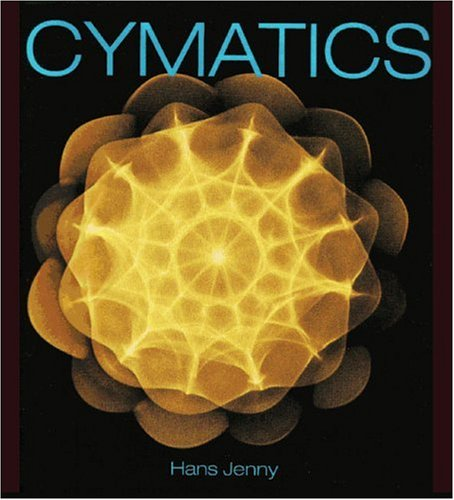
\includegraphics[width=0.5\textwidth]{chap1/figures/cymatics.jpg}
\caption{\em One of the visual patterns from Hans Jenny's seminal text.}
\label{fig:cymatics}
\end{figure}

This dissertation serves as a bridge between generative art and sound, computer graphics, and cymatics. Using computational fluid dynamics simulations as our background data, we define a bridge between the visual
and sonic results in the spirit of cymatics, linking resonant visual shapes of vibration to their corresponding audio frequencies. Along the way, we devise a data compression algorithm as part of the simulation pipeline to
ease the computational load. 

\section{Systems of Sonification and Aesthetic Goals}
The term ``sonification'' has many subtly different interpretations and definitions, but we use it in this dissertation to refer broadly to the association of data to sound. Scientifically-focused sonifications can reveal underlying
qualitative patterns in the data, while artistic-focused sonifications can serve as a framework for composing novel musical or even audiovisual works. In this dissertation, we use the phenomenon of fluid dynamics as our
data, focusing on a system of sonification that, while revealing certain qualitative features of the fluid motion, mostly serves to generate novel audiovisual pieces. More precisely, we use the the {\em subspace} method of simulation \cite{Treuille:2006:MRF}, based on a stable computational fluid dynamics simulation, as our data, and a model-based sonification system to associate the data with musical sound. Such a sonification system is analogous to the resonant modal shapes and 
frequencies as discovered by Chladni and Jenny in the field of cymatics.

\section{Data Compression and Memory Obstacles with Subspace Matrices}
The general technique of data compression began with Claude Shannon \cite{shannon1998mathematical} and the field of information theory \cite{cover2012elements}. It is of practical relevance for many problems in computing, as reducing memory footprints
can make certain simulations more feasible to run. The general idea of data compression is that by exploiting patterns or redundancies in data, we can often represent the same data in a more terse form.
A wide variety of research in this area has produced many successful compression schemes, from lossless compression of arbitrary files (ZIP) to lossy compression of image (JPEG), audio (MP3), and video (MPEG) \cite{ziv1977universal, wallace1992jpeg, iso1993iec, le1991mpeg}.

The subspace method of simulation \cite{Pentland:1989:GVM}, while known to achieve large speedups over regular full-space simulations, also requires a potentially prohibitive memory cost, consuming dozens of gigabytes of RAM 
in high-resolution, three-dimensional simulations. While other research has been done on compressing blendshape matrices for facial animations \cite{Seo:2011:CDM} and eigenmode matrices for modal sound synthesis \cite{Langlois:2014:ECM},
to our knowledge, no previous work on compressing fluid subspace matrices has been done.

\section{Thesis Statement and Main Results}
The thesis statement is as follows:

\begin{addmargin}[1em]{2em}
{\em The method of subspaces in computational fluid dynamics for computer graphics can be leveraged to systematically produce artistic audiovisual pieces.}
\end{addmargin}
In particular, I demonstrate three main results:

\begin{itemize}
	\item I propose a versatile system of sonification of fluid subspaces.
	\item I describe a data compression algorithm for fluid subspaces to help ease high computational costs.
	\item I demonstrate the sonification system with several audiovisual {\'e}tudes.
\end{itemize}

The first result, the sonification system, achieves a two-way coupling between sound and visual, allowing the visual to drive the sound, the sound to drive the visual, or even a third intermediary process to govern both the sound and visual simultaneously. The flexibility of the system allows the composer to generate a variety of sounds and visual forms that are nonetheless intertwined in a common language. 

The second result, the data compression algorithm, achieves an order of magnitude compression of fluid subspace matrices needed in memory during runtime without any perceivable visual artifacts. The main result is the technique behind the compression scheme, a transform-based algorithm, combined with a novel sparse frequency-domain projection and reconstruction.

The third result, the audiovisual {\'e}tudes, serve as proof of concept of the possibility of the sonification system as a means toward developing an audiovisual language. Carefully chosen parameters are modulated to demonstrate compositional gestures that can be achieved in both the audio and visual domain. 

\section{Organization}
The dissertation is organized as follows. Chapter \ref{chap:chap2} provides background and related work in the domain of generative art and sonification. Chapter \ref{chap:chap3} gives additional background in the domain of fluid simulation for computer graphics, focusing in particular on the method of subspaces. Chapter \ref{chap:chap4} describes the data compression algorithm for fluid subspaces and shows its effectiveness on a variety of different subspace simulations. In Chapter \ref{chap:chap5} we describe the system of sonification of the fluid subspaces. Chapter \ref{chap:chap6} demonstrates the versatility of the sonification system through a series of systematic audiovisual {\'e}tudes. Finally, Chapter \ref{chap:chap7} presents conclusions and directions for future work.

\chapter[Related Work]{Related Work}
\section{Sonification and Generative Art}

The question of mapping computational fluid dynamics data into sound belongs to the intersection of the domains of {\em sonification} and {\em generative art}. Sources vary in agreement on the definition of sonification. According to Hermann, sonification is ``the technique of rendering sound in response to data and interactions.'' \cite{hermann2011sonification} Kramer et al.~define it as ``the use of nonspeech audio to convey information.'' \cite{kramer2010sonification} We shall make a distinction between {\em scientific} sonification, which aims primarily toward conveying information clearly, and {\em musical sonification}, which aims primarily toward aesthetically useful generation of music. There are many possible strategies for sonification, including audification, parameter mapping sonification, and model-based sonification. \cite{hermann2011sonification} 

Generative art is sometimes thought of in very general terms. For instance, Boden specifies eleven different categories of generative art: electronic art, computer art, computer-assisted art digital art, generative art, computer-generated art, evolutionary art, robot art, interactive art, computer-interactive art, and virtual reality art. \cite{boden2009generative}. In the text, however, we prefer a more narrow definition of generative art as art which has been created through the design and use of a computational system.

One of the main attractions of this compositional style is the possibility of novel discoveries that go beyond what the artist may otherwise have been able to conceive: ``The computer can allow a composer to write music that goes beyond that which she is already capable of.'' \cite{roads2015composing}

\subsection{Aesthetics}
A continual dilemma in generative art is the conflict between the level of rigor of the underlying formal system and the human perception of its output. Some artists (e.g. Milton Babbitt) take the dogmatic position that the otic of the system trumps the general perception of the output. \cite{babbitt1958cares}  However, others such as K{\v{r}}enek have taken a more careful middle ground, arguing that the existence of an aesthetically coherent system of rules is no guarantee that an aesthetically coherent artistic result will perceptibly emerge: ``We cannot take the bare logical coherence of a musical `axiomatic' system as the sole criterion of its soundness! \dots The outstanding characteristic of music [is] its independence from the linguistic limitations of general logic.'' \cite{kvrenek1939music}
\chapter[Background]{Background}
\label{chap:chap3}
\section{Fluids}

A {\em fluid}, formally speaking, is a substance that continuously deforms under the application of shear stress. \todo{citation}. More intuitively, it is a substance that {\em flows}. Although colloquially we may use the term fluid to refer only to liquids, gases can exhibit flow, and are therefore considered to be fluids as well. (Indeed, the results demonstrated in this dissertation focus entirely on the turbulent flow of smoke.) The natural world is full of captivating fluid motions: ocean waves, ripples in a pond, clouds, the steam of a teakettle, etc. These flowing patterns, while beautiful, appear difficult to formalize precisely, and the modeling of fluids continues to be a mathematical and computational challenge to this day.

\section{Physics-based modeling}
The field of {\em fluid dynamics} in physics seeks to model and describe fluid flow systematically according to equations generated from a set of basic assumptions and principles. In order for continuous mathematical operators to be used to describe fluids, one of the basic assumptions is that of the {\em continuum}: for mathematical purposes, we assume that fluid velocity varies continuously across space, even though in reality, fluids are actually composed of discrete molecules. TBesides this continuum assumption, the various conservation laws of mass, energy, and momentum, imply the famous Navier-Stokes equations, which describe the velocity field $\uu$ of fluid flow depending on the intrinsic stress of viscosity and pressure. In the case where we make the additional simplifying assumption that the fluid is incompressible,\footnote{i.e., the fluid density does not vary within the flow field} the equations take the following form:

\begin{equation}
\label{eq:incompress}
\nabla \cdot \uu = 0
\end{equation}
\begin{equation}
\label{eq:momentum}
\frac{\partial \uu}{\partial t} = -\left(\uu \cdot \nabla \right)\uu + \nu \nabla^{2}\uu - \nabla{p} + \mathbf{f}_e
\end{equation}

There are several terms here that must be unpacked:

\begin{itemize}
\item The time-varying vector field $\uu = u(\xx, t)$ describes the fluid velocity field. It is the main quantity we are interested in, and solving these differential equations amounts to figuring out what $\uu$ is for all times $t$.
\item The constant $\nu$ represents the viscosity of the fluid, which represents its resistance to deform while flowing. (Intuitively, this can be thought of its resistance to being stirred: molasses, for instance, has higher viscosity than water.) 
\item The time-varying scalar field $p = p(\xx, t)\ $ represents the pressure field of the fluid. 
\item The time-varying vector field $\mathbf{f}_e = \mathbf{f}_e(\xx, t)$ represents any external forces affecting the fluid, such as gravity.
\end{itemize}
Equation \ref{eq:incompress} enforces the assumption of incompressibility, while equation \ref{eq:momentum} is a consequence of the aforementioned conservation laws.

\section{Simulation}

Simulation is, of course, the imitation of a natural process, in this case over time. Any simulation must first determine a technique of modeling the process computationally, and there are often many different possible strategies. We consider here a few typical approaches in computational fluid dynamics.

One of the most direct ways of modeling fluids is to discretize both the spatial and time domain. In other words, to perform the calculations, we dice up the region of space into a regular grid of small cubical cells. Each cell then contains a vector, or arrow, describing the velocity of the fluid at the position in space. In order to evolve the motion of the flow over time, we also dice up time itself into a sequence of discrete time steps, computing how the velocity of the fluid in each cell changes at each time step. This approach is called the {\em Eulerian} viewpoint of the flow. Intuitively, this can be thought of as staying in a fixed location and observing the flow through that particular location. More precisely, the fluid's velocity in this viewpoint is represented as $\uu(\xx, t)$, which gives the velocity of the fluid at each spatial location $\xx$ and time $t$.

In contrast, the {\em Lagrangian} viewpoint of the flow takes the point of view of each individual fluid particle as it moves along the flow through space and time. Intuitively, this can be thought of drifting along with the flow. If we label each particle based on its position in space using a vector field $\mathbf{r}$, we then describe the fluid flow with the position field $\mathbf{X}(\mathbf{r}, t)$ , which gives the position of each particle labeled by $\mathbf{r}$ at time $t$.

We can connect these two viewpoints with the following equation:
\begin{equation}
\label{eq:euler-lagrange}
\uu\left(\mathbf{X}\left(\mathbf{r}, t\right)\right) = \frac{\partial \mathbf{X}}{\partial t}\left(\mathbf{r}, t\right)
\end{equation}

The left-hand side of equation \ref{eq:euler-lagrange} describes the velocity of the flow at position $\mathbf{r}$ and time $t$ using the Eulerian-specified velocity field $\uu$, while the right-hand side describes the same velocity by taking the partial derivative of the Lagrangian specified position field $\mathbf{X}$.

Given an Eulerian-specified fluid velocity field $\uu(\xx, t)$ over a domain of space, and given another Eulerian-specified scalar field $\varphi(\xx, t)$ (e.g., temperature) over the same domain, we can consider the total derivative of $\varphi$. By the chain rule, this expands as follows:

\begin{equation}
\frac{\mathrm{d}}{\mathrm{d}t}\varphi\left(\xx, t\right) = \frac{\partial \varphi}{\partial t} + \dot{\xx} \cdot \nabla \varphi
\end{equation}

The partial derivative term $\frac{\partial \varphi}{\partial t}$ indicates the instantaneous rate at which the temperature is changing with time, holding the spatial position constant. Thus, if we imagine a fluid flow being comprised of many infinitesimal particles, this term represents any change in temperature of a particle at a fixed spatial location. The remaining term $\dot{\xx} \cdot \nabla \varphi$ describes a more dynamic rate of change, as it incorporates changes in temperature caused by moving {\em along} the flow through the path $\dot{\xx}$. This movement is in the Lagrangian spirit of drifting along with the flow. In the case where $\dot{x}$ is taken to align with the flow velocity $\uu$, we have 

\begin{equation}
\frac{\mathrm{d}}{\mathrm{d}t}\varphi\left(\xx, t\right) = \frac{\partial \varphi}{\partial t} + \uu \cdot \nabla \varphi
\end{equation}
which is often called the {\em material derivative}. The operator $\uu \cdot \nabla$ is the advection operator, which we will be prominent later on.

\subsection{Numerical Simulation}
Numerical simulation brings the abstract equations of mathematical simulation to a concrete, computational implementation. Typically, this involves discretization of any continuous parameters in the model, such as time and 
space. As such, idealized concepts such as spatial and time-dependent derivatives must be approximated. Numerical analysis is a broad and rich field in applied mathematics and engineering, and many different approaches
are available, each with various pluses and minuses. For the scope of this dissertation, we consider the numerical method of Jos Stam's {\em Stable Fluids} \cite{Stam99}, which is the backbone of our full-space fluid simulation technique. 

The first step in Stam's method, following the technique of Chorin and Marsden \todo{citation}, is to devise a technique to combine the two equations \ref{eq:incompress} and \ref{eq:momentum} into one equation. We rely on a result from vector calculus called the Helmholtz-Hodge decomposition, which states that any arbitrary vector field $\ww$ can be decomposed uniquely into the sum of a divergence-free, or solenoidal, vector field and a curl-free, or irrotational, vector field. More precisely,
we can write

\begin{align}
\label{eq:hh}
\ww &= \uu_{\text{solenoidal}} + \uu_{\text{irrotational}}\\
        &= \uu_{\text{solenoidal}} + \nabla q
\end{align}
since the curl $\nabla \times \nabla q$ must be zero for some scalar field $q$. Hence, we can define a projection operator $P$ which maps a vector field to its (unique) solenoidal component. In other words,
$P \ww = \uu_{\text{solenoidal}}$. Indeed, this operator can be discovered explicitly by taking the divergence of both sides:

\begin{equation}
\nabla \cdot \ww = \nabla^2 q
\end{equation}
which is a Poisson equation for the scalar field $q$. Given $\ww$, we can solve this equation to obtain $q$, and then compute $\uu_{\text{solenoidal}}$ via $\uu_{\text{solenoidal}} = \ww - \nabla q$. Thus, we can take the
second equation in the Navier-Stokes equations, \ref{eq:momentum}, and apply the projection operator $P$ to both sides, obtaining

\begin{equation}
\label{eq:stamns}
\frac{\partial \uu}{\partial t} = P\left(-\left(\uu \cdot \nabla \right)\uu + \nu \nabla^{2}\uu + \mathbf{f}_e\right)
\end{equation}
This conveniently eliminates the pressure term $\nabla p$ and unites the two equations \ref{eq:incompress} and \ref{eq:momentum} into one.

The next important technique that Stam's method uses involves {\em splitting} the operators in the Navier-Stokes equations \ref{eq:stamns} into a sequence of simpler operators. In other words, because the right-
hand-side of \ref{eq:stamns} can be regarded as a combination of several terms (namely, an advection term, a diffusion term, an external forces term, and a projection) \ref{eq:splitting}, we focus our attention on solving each of these simpler differential equations in isolation. Once we have a solution to each individual term, we can construct an approximation for the solution to the more complex full equation \ref{eq:stamns}. Establishing some notation, suppose we begin from an initial state $\uu_0 = \uu(\xx, 0)$ and would like to step forward in time by a timestep $\Delta t$. Beginning from the previous timestep's solution $\ww_0 = \uu(\xx, t)$, we solve a sequence of equations $\ww_0, \dots, \ww_4$, ending with the last velocity field which is equal to the value at the next time step: $\ww_4(\xx) = \uu(x, t + \Delta t)$. Iterating this procedure generates a complete numerical solution, as desired.

\begin{equation}
\label{eq:splitting}
\ww_0(\xx) \xrightarrow{\text{add forces}} \ww_1(\xx) \xrightarrow{\text{advect}} \ww_2(\xx) \xrightarrow{\text{diffuse}} \ww_3(\xx) \xrightarrow{\text{project}} \ww_4(\xx)
\end{equation}

The external forces can be approximated simply using forward Euler or other explicit schemes. In other words, we can write
$\ww_1(\xx) = \ww_0(\xx) + \Delta t \mathbf{f}_{\text{ext}}(\xx, t)$. The advection term, however, is nonlinear and adds considerable complexity to the solution. Stam's insight was to consider the advection from a Lagrangian viewpoint. Intuitively speaking, each fluid particle is advected by its own velocity. Hence, to calculate the velocity at a particular spatial point $\xx$ at the next time step $t + \Delta t$, we backtrace from the point $\xx$ through the previous velocity field over a time step of $\Delta t$. Letting $\xx$ vary, following Stam's notation, this defines a path $\mathbf{p}(\xx, s)$ along a partial streamline of the velocity field. We assume then that the new velocity at the point $\xx$ at time $t + \Delta t$ must therefore be the same as the old velocity at the backtraced point at time $\Delta t$ previous. (Although the backtraced point may not lie exactly on a grid cell, we can use linear interpolation to reslve this problem.) More concretely, we have $\ww_2(\xx) = \text{Interpolate}\left(\ww_1\left(\mathbf{p}(\xx, -\Delta t)\right)\right)$.

One of the key advantages to Stam's advection technique is that it is {\em unconditionally stable}: in other words, no matter how large a time step $\Delta t$ we select, the velocity will remain bounded. Intuitively, this is straightforward to observe: each velocity update is the result of an interpolation of previous velocity values, and therefore cannot be any greater than any of the previous values. From a practical standpoint, this numerical stability is a big plus; however, with very large time steps, the problem of numerical dissipation becomes more of an issue. A more detailed discussion of these issues can be found in \todo{citations}

Within Stam's paper is another interesting topic of carrying out the equations of motion within the Fourier domian. Although 
we do not implement our solver using this technique, it is a topic of interest based on our compression technique as well as,
our frequency-domain interpretation of the fluid modes and our corresponding sonification technique later on, so we delve into a few details here. The key observation is that the Fourier transform diagonalizes spatial derivatives. In other words, if we denote the Fourier transform of $\uu(\xx)$ by $\fancyF[\uu(\xx)](\kk) = \uhat(\kk)$, then we have $\fancyF[\nabla \uu(\xx)](\kk) = i \kk \uhat(\kk)$. The divergence operator similarly satisfies $\fancyF[\nabla \cdot \uu(\xx)](\kk) = i \kk \cdot \uhat(\kk)$, and the Laplacian, being the divergence of the gradient, satisfies $\fancyF[\nabla^2 \uu(\xx)](\kk) = - k^2 \uhat(\kk)$, where $k = |\kk|$. The upshot of all this is that we can view some of the fluid operators in the spatial domain in simple ways in the frequency domain. For example, the diffusion, based on the Laplacian operator, can be thought of as a low-pass filter with decay governed by the viscosity. In general, this mode of
thinking bears fruit later for our discussions of the compression algorithm in Chapter \ref{chap:chap4} and our sonification system in Chapter \ref{chap:chap5}.

\section{Subspace Methods}
Subspace methods, also known as model reduction, or reduced order methods, has a long history in engineering and applied mathematics, including applications to fluid simulation \cite{lumley1967}, and was introduced to the computer graphics literature in 1989 by Pentland and Williams \cite{Pentland:1989:GVM, Berkooz93theproper}. The basic principle of these methods, as the name suggests, is to reduce the computational complexity of a large numerical simulation. A typical simulation will have many degrees of freedom in principle, generating a vast state space of possibilities. However, in practice, not all of these degrees of freedom are of equal importance. By systematically discovering a reduced subspace of the state space, and carrying out calculations within this subspace, a subspace simulation can lead to large computational accelerations with minimal degradation of accuracy.

\subsection{Modal Analysis}
To see an example of the subspace method in action, consider the modeling of small deformations of rigid bodies. Although rigid bodies in principle have many degrees of freedom over which they can deform, they have certain characteristic shapes into which they are more likely to deform. These shapes, also known as {\em modes}, are the ones which minimize the strain, and in an intuitive sense are the ``natural'' deformations of the rigid body. To compute these, we assume the rigid body is discretized into a mesh with $N$ vertices. We then compute the system mass and stiffness matrices $\MM \in \R^{3N \times 3N}$ and $\KK \in \R^{3N \times 3N}$, respectively. The modes then satisfy the generalized eigenvalue equation

\begin{equation}
	\KK \xx = \lambda \MM \xx
\end{equation}

Due to the special properties of the matrices $\MM$ and $\KK$, which are both symmetric positive-definite (SPD), the eigenvalues $\lambda_i$ are positive real numbers. 
Although there are $3N$ eigenvalues in total, in practice, we can take a subset of them, $\lambda_1, \lambda_2, \dots, \lambda_r$, from least to greatest, and their associated eigenvectors
 $\psi_1, \psi_2, \dots, \psi_r$. (Here, $r \ll 3N$ represents the number of modes we wish to retain.) The eigenvectors $\psi_i$ we choose corresponding to the eigenvalues $\lambda_i$ 
 are not unique; for convenience, we select those that satisfy the mass-orthogonality condition $\langle \MM \psi_i, \psi_j \rangle = \delta_{ij}$, where $\delta_{ij}$ is the Kronekcer delta, 
 equaling $0$ for $i \neq j$ and $1$ for $i=j$. The $r$-dimensional subspace $S \subset \R^{3N}$ formed by the linear span of these eigenvectors can be encapsulated in matrix form 
 by assembling the modal basis matrix $\UU \in \R^{3N \times r}$ as follows:

\begin{align}
	\UU^{T} &= \begin{pmatrix}
	\vertbar & \vertbar &   & \vertbar \\
	\psi_1 & \psi_2 & \dots & \psi_r   \\
	\vertbar & \vertbar &   & \vertbar
  \end{pmatrix}
\end{align}

Thus, the mass-orthogonality condition we specified for the modes can be captured in the more succinct matrix form $\UU^{T} \MM \UU = \II_r$,
where $\II_r \in \R^{r \times r}$ denotes the $r \times r$ identity matrix.

Now consider the typical equation of motion for undamped small deformations $\xx \in \R^{3N}$ corresponding to external forces $\ff \in \R^{3N}$: 
\begin{equation}
\label{eq:mass-spring}
\MM \ddot{\xx} + \KK \xx = \ff
\end{equation}

Equation \ref{eq:mass-spring}, is a very high-dimensional linear differential equation obtained by applying the standard equations of elastic deformation to the mesh with $3N$ nodes using the finite element method (FEM). For very fine meshes with large values of $N$, this equation may present a computational bottleneck. Hence, the approach of model reduction is welcome. We proceed by approximating $\xx$ as a linear combination of the modes $\psi_1, \dots, \psi_r$:

\begin{equation}
\xx \approx \UU \qq
\end{equation}
where the vector $\qq \in \R^{r}$ has components $q_i$ that are the corresponding weights of the associated modes $\psi_i$, $i=1,\dots,r$. This vector $\qq$ is called the {\em reduced coordinates} of $\xx$, and can also be thought of as the projection of $\xx$ into the subspace $S$. Rewriting equation \ref{eq:mass-spring}, we obtain

\begin{equation}
\MM {\UU \ddot{\qq}} + \KK \UU \qq = \ff
\end{equation}
By the generalized eigenvector condition, we have $\KK \UU = \Lambda \MM \UU$, where $\Lambda = \textnormal{diag}\left(\lambda_1, \dots, \lambda_r\right)$. Hence, we simplify as follows:

\begin{equation}
\MM \UU \left(\ddot{\qq} + \Lambda \qq\right) = \ff
\end{equation}
Next, to clear away the factor of $\MM \UU$, we pre-multiply both sides by $\UU^{T}$:

\begin{equation}
\UU^{T} \MM \UU \left(\ddot{\qq} + \Lambda \qq\right)= \UU^{T} \ff
\end{equation}
By the mass-orthogonality condition, the term $\UU^{T} \MM \UU$ reduces to $\II_r$.  On the right-hand-side, $\widetilde{\ff} = \UU^{T} \ff \in \R^r$ is the reduced form of $\ff$. Hence, we have the following lower-dimensional linear differential equation with unknown $\qq \in \R^{r}$:

\begin{equation}
\ddot{q} + \Lambda \qq = \widetilde{\ff}
\end{equation}
In this particular case, the system is uncoupled since $\Lambda$ is diagonal, so we have a collection of $r$ independent one-dimensional ordinary differential equations. These can be integrated forward in time very efficiently, obtaining $\qq_{t+1}$, the value of $\qq$ at the next time step. To finish the computation, we reconstruct into the full-dimensional space by computing $\xx_{t+1} = \UU \qq_{t+1}$.

\subsection{Sound generation}
Small rigid deformations of a solid body are precisely those that generate sound waves, so we briefly consider the application to audio of the previous discussion. Recall that our subspace reduction produces a collection of $r$ independent one-dimensional equations, which, expanded out, take the form

\begin{equation}
\label{eq:system}
\ddot{q_i} + \lambda_i q_i = \psi_i^{T} f_i, \ \ i = 1, \dots, r
\end{equation}

Recalling that each $\lambda_i$ is a positive real number, let $\omega_i$ be the positive square root $\omega_i = \sqrt{\lambda_i}$. Then the general analytical solution to the homogenous portion of each one-dimensional differential equation in \ref{eq:system} is given by $q_i = c_1 e^{i \omega_i t} + c_2 e^{i \omega_i t}$. In other words, we can think of the $i$-th mode as resonating at a natural frequency of $\omega_i$. This allows us to perform simple additive synthesis by mixing together a collection of sinusoids at the corresponding frequencies, generating the audio signal that corresponds to the physical deformation. The spirit of this basic approach motivates
our sonification process in Chapter \ref{chap:chap5}.

\subsection{A more general subspace formulation}

\chapter[Transform-based compression of fluid subspaces]{Transform-based compression of fluid subspaces}

In the previous chapter, we discussed the potential for subspace methods to accelerate the computational cost of physics-based simulations. However, a significant drawback of the subspace approach is the time/memory tradeoff: the speed increase comes at a cost of much larger memory requirements. Specifically, subspace simulations can easily consume dozens of gigabytes of memory when dealing with high-resolution scenes. In this chapter, we discuss a compression method to reduce the memory footprint of subspace methods by an order of magnitude. 

\section{Previous Work}
Since memory consumption is a known challenge with subspace techniques, other research has focused on reducing the memory footprint of these simulations. In the applications of sound \cite{Langlois:2014:ECM} and blendshape matrices \cite{Seo:2011:CDM}, compression techniques have been developed; however, we are unaware of analogous research in subspace fluid simulation. In the work of Wicke et al.~\cite{Wicke:2009}, a modular fluid basis is used that can be tiled throughout the domain. However, our approach is complementary, as the modular tiles themselves could be further compressed by applying our algorithm.

\section{Background}
\subsection{Data Compression Preliminaries}
The general problem of data compression at first blush seems daunting: how do we reduce the memory footprint of a set of data without losing information? Fortunately, the sets of data that we typically work with are not random, but rather contain many patterns and redundancies. Exploiting these redundancies is the key to any successful data compression algorithm.

Data compression algorithms can be divided into two distinct families: lossless and lossy. A lossless compression algorithm is able to take an input signal, compress it, and reconstruct the exact same input signal. A simple example is run-length coding. For instance, to represent 100 white pixels, followed by 200 black pixels, followed by an another 50 white pixels, we can code the sequence (`w', 100), (`b', 200), (`w', 50), rather than coding the 350 pixels individually. Decoding is straightforward and retains all information. The ZIP file format is a familiar example of widely-used lossless data compression.

Lossless compression can be very powerful when applied to original data with many redundancies; however, it has strict limitations based on the mathematics of information theory. Every file, no matter how redundant, contains a certain amount of information. \todo{Add details about information theory/entropy.}

Lossy compression, by contrast, may not be able to reconstruct the exact same input signal. Its applications tend to focus on perceptual data, such as images, video, and sound. Although its reconstructions are not perfectly faithful, if the technique is soundly based on the limits of human perception, the results are virtually indistinguishable. The JPEG file format for images is a widely-used lossy data compression algorithm.

Data streams of images oftentimes contain more information than a human can reasonably resolve. For example, a picture might contain fine details that are indistinguishable from their smoothed counterpoints, or subtle color gradients that are indistinguishable from coarser ones. The key to most lossy data compression algorithms is finding a way of transforming the original information into a domain that captures these characteristics more naturally. These techniques are called {\em transform coding}.

\subsection{Mathematical Preliminaries}
In order to describe transform coding formally, we will require several notions from linear algebra and analysis.
\subsubsection{Vector Spaces}
The basic framework of most of our data manipulation can be expressed through the notion of vector spaces. We are familiar with the physical notion of vectors in two- or three-dimensional space as quantities with both a magnitude and a direction, often depicted graphically with an arrow. \todo{Add figure of a 2D vector.} For convenience, we often represent vectors using coordinates. We can view the coordinate representation as a decomposition into fundamental unit vectors pointing in the $x$ and $y$ direction. These are called the {\em basis} vectors. Any arbitrary vector can be decomposed uniquely into a combination of these basis vectors. 

Vectors can be added or subtracted, producing another vector. They can also be multiplied by a scalar (i.e.,~a number in $\R$ or $\C$), yielding another vector. The formalization of this idea is the mathematical concept of a {\em vector space}, which allows for a more abstract treatment of vectors. For example, an image represented on a computer as a sequence of $N$ pixel values can be regarded as a vector living in the vector space $\R^N$. This abstraction allows us to bring the tools of linear algebra to bear on a variety of seemingly different applications.

\subsubsection{Inner Products}
Recall that an {\em inner product}, or dot product, is a binary operation $\langle \cdot, \cdot \rangle$ between two vectors that yields a scalar as an output. The most familiar example is in $\R^2$, where, given two vectors $\vv = (v_1, v_2)$ and $\ww = (w_1, w_2)$, we have $\langle \vv, \ww \rangle = v_1w_1 + v_2w_2$. Inner products add a notion of geometry to a vector space through angles and length: when an inner product between two vectors is $0$, the vectors are orthogonal; and the inner product of a vector with itself gives the square of its length. For example, the basis vectors $\ee_x = (1, 0)$ and $\ee_y = (0, 1)$ are orthogonal, and the vector $\vv = (3, 4)$ has squared length $\langle \vv, \vv \rangle = 3^2 + 4^2 = 5^2$. Inner products also are closely related to the projection of one vector onto another. For example, if we take an arbitrary vector $\vv = (v_1, v_2)$ and take its inner product with the basis vector $\ee_y = (0, 1)$, the result is the component $v_2$ in the $y$ direction. In general, given a set of unit basis vectors which are mutually orthogonal (known as an {\em orthonormal} basis), we can compute the various components of arbitrary vectors by calculating their inner products with the corresponding basis vector.

Besides the familiar inner product in $\R^2$, more general inner products exist in other vector spaces. The canonical inner product in $\C^n$ is given by $\langle \vv, \ww \rangle = \displaystyle \sum_{k=1}^{n}v_k\overline{w_k}$, where the overbar denotes the complex conjugate. The conjugate may seem strange, but is necessary to preserve the notion that taking an inner product of a vector with itself should give the squared length of the vector. The canonical inner product in the function space $L_2([-\pi, \pi])$, the space of functions on the interval $[-\pi, \pi]$ with finite energy, is given by $\langle f, g \rangle  = \displaystyle \int_{-\pi}^{\pi}f(x)\overline{g(x)}dx$.

\subsubsection{The Discrete Fourier Transform}


\subsection{The JPEG Coding Algorithm}
\chapter[Visualizing and sonifying fluid subspaces]{Visualizing and sonifying fluid subspaces}
\label{chap:chap5}

Note: A large portion of this chapter has previously appeared as \cite{bridges2017:305}
\bigskip\bigskip

%%%%%%%%%%%%%%%%%%%%%%%%%%%%%%%%%%%%%%%%%%%
\begin{figure}[H]
		\centering
		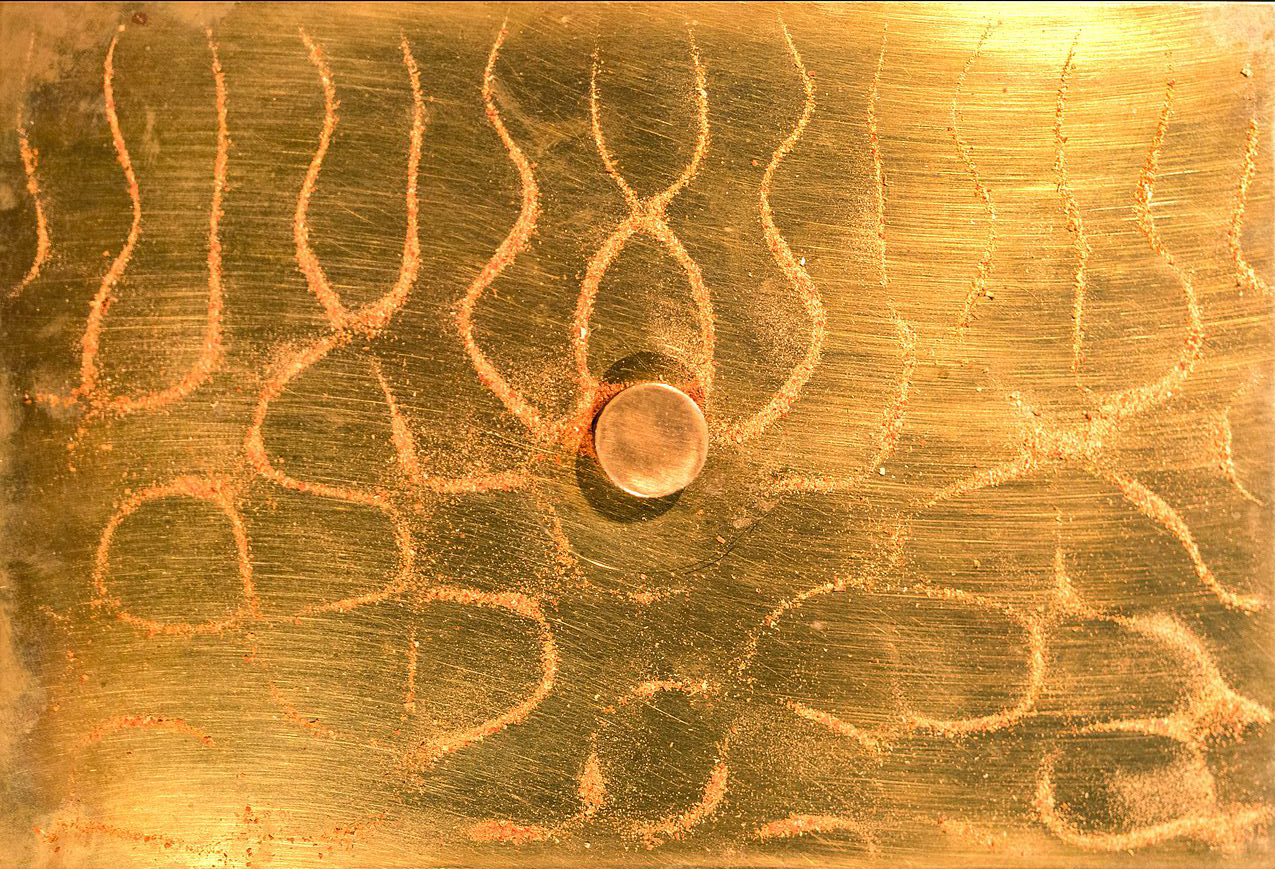
\includegraphics[height=0.3\textwidth]{chap5/figures/chladni_plate.jpg}
		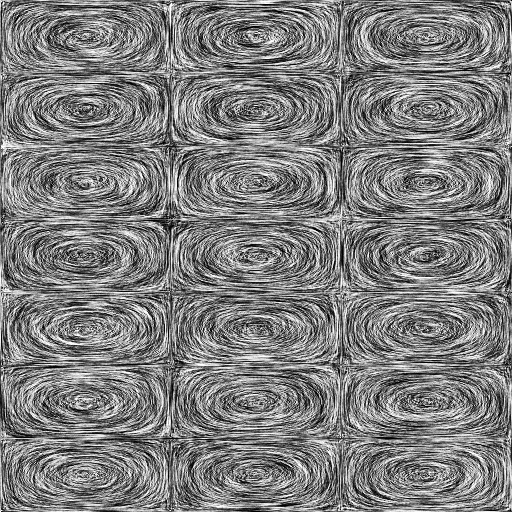
\includegraphics[height=0.3\textwidth]{chap5/figures/LIC.jpg}
%		\vspace*{-1em}
		\caption{{\em{\bf Left:} Chladni patterns realized through a physical experiment. Source: Wikimedia Commons.} {\em{\bf Right:} Analytic $\twoD$ eigenvector of the Navier-Stokes equations using the method of de Witt et al.} \cite{deWitt:2012}.}
		\label{fig:chladni-plate}
\end{figure}

\section*{Introduction}
Chladni plates reveal beautiful patterns when vibrated at specific frequencies (Figure \ref{fig:chladni-plate}). Both the spatial patterns and sonic frequencies that arise have long been known to have intimate connections to the eigenvectors and eigenvalues of an idealized rigid plate. For this idealized case, closed form expressions can be obtained, and the eigenvalues are known to correspond to the audio spectrum emitted by the plate. In this work, we seek to explore a generalization of this phenomenon by applying a similar procedure to a more complex scenario: a turbulent computational fluid dynamics (CFD) simulation.

Unlike the Chladni plate case, closed form expressions are not available for the eigenvectors of an arbitrary CFD simulation, so we instead discover a set of ``empirical'' eigenvectors. The natural connection between eigenvalues and audio frequencies in the Chladni plate case is also no longer present, so we instead construct a sonification to produce a mapping between fluid trajectories and sound. Using this approach, we obtain a variety of organic forms that have a unique visual character and generate associated sounds that unfold over rich spectral envelopes. Our ability to to directly control the spatial and audio frequency spectrum allows the potential for a mathematically principled artistic exploration of the audiovisual space through the medium of short film, which we demonstrate with several brief preliminary results.

% intro to eigenvectors and eigenvalues

%These eigenvectors can be computed analytically, as they correspond to very small deformations (i.e.~vibrations), and can be written in terms of a single differential operator over a square domain \cite{gander2012euler}. These visual representations can be extended to more complex scenarios, where the eigenvectors and their corresponding eigenvalues are instead computed numerically. In this work, we compute the eigenvectors of a dynamic computational fluid dynamics simulation, which involves large deformations instead of small vibrations, and the Navier-Stokes equations in lieu of a single differential operator. We then visualize the turbulent motion of the eigenvectors in this spectral representation and construct a sonification of the resulting frequencies to produce a mapping between fluid trajectories and sound. The results are organic visual forms with a unique character and a variety of associated sounds that unfold over rich spectral envelopes.


\begin{figure}[H]
		\centering
		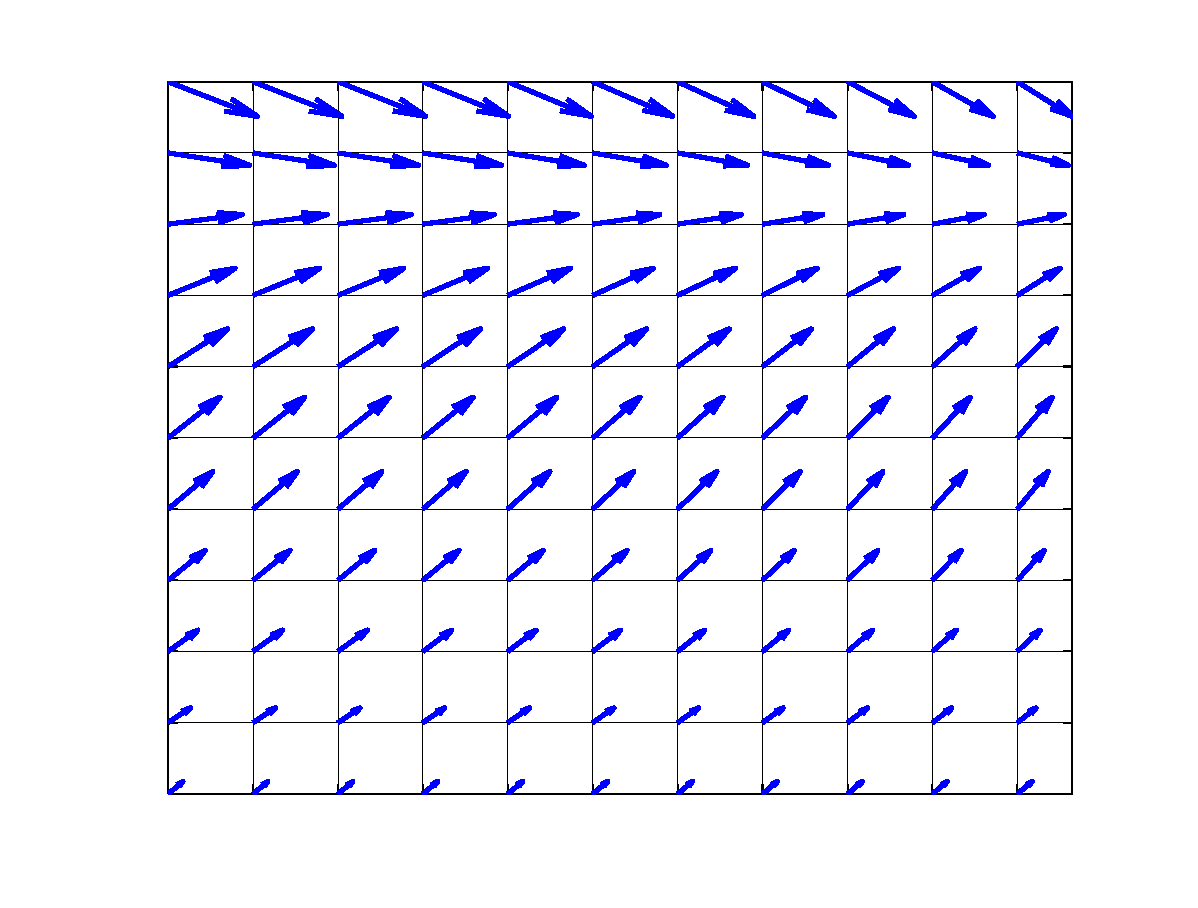
\includegraphics[height=0.3\textwidth]{chap5/figures/velocity_2d.eps}
		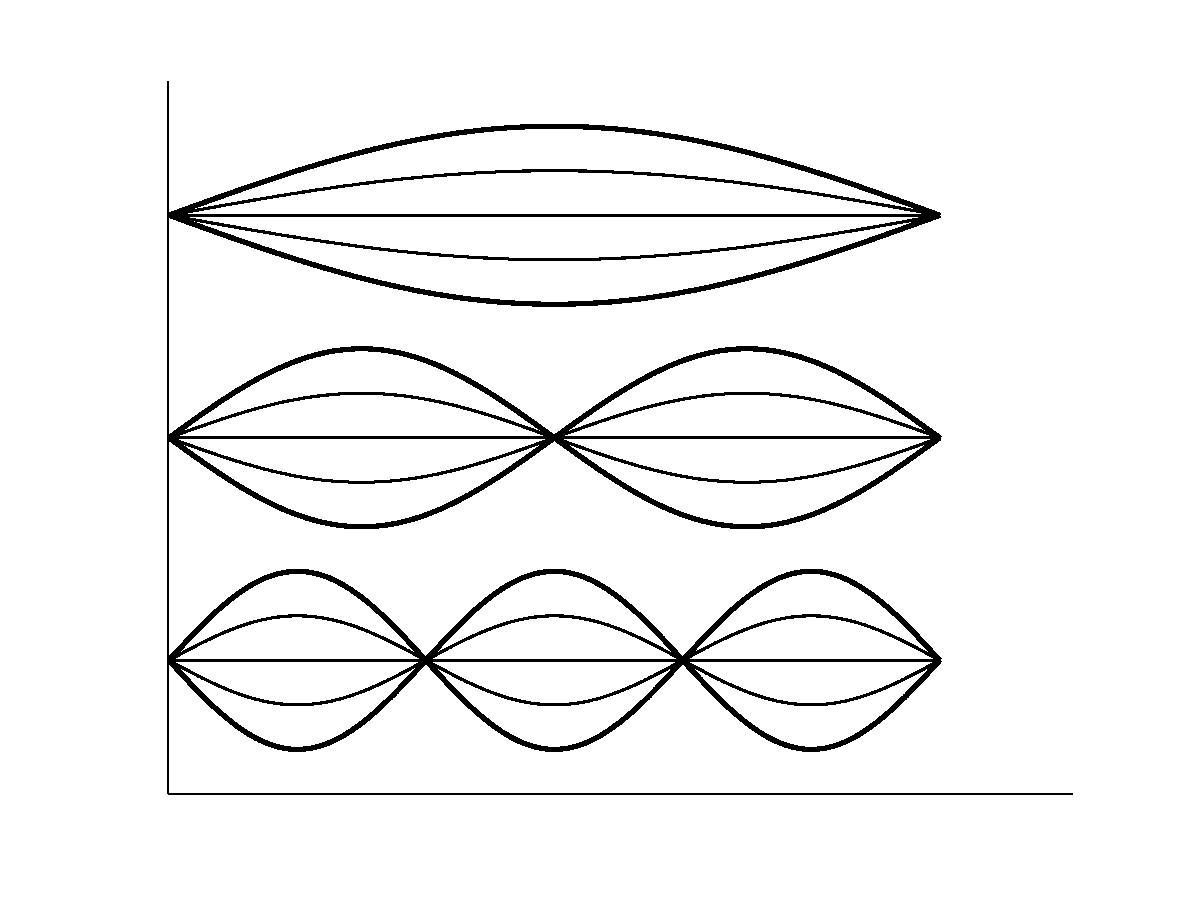
\includegraphics[height=0.3\textwidth]{chap5/figures/guitar_modes.eps}
		\caption{{\em{\bf Left:} A $\twoD$ velocity field over a regular grid.} {\em{\bf Right:} From top to bottom, the modes of vibration of a guitar string for $N=1, 2, 3$.}}
		\label{fig:velocity-field}
\end{figure}

\section*{Eigenvector Preliminaries}
In order to better understand the role they play in this work, we start with a review of eigenvectors and values. The eigendecomposition of a square matrix $\boldA$ is usually written as $\boldA = \boldQ \Lambda \boldQ^T$. The matrix $\Lambda$ is zero except along its diagonal, and each individual entry along the diagonal is an ``eigenvalue,'' where the German {\em eigen} roughly translates to ``characteristic.'' The matrix $\boldQ$ is generally not diagonal, and contains columns that are each considered an ``eigenvector'' of $\boldA$. The essential character of the matrix is captured by these vectors and values because they satisfy a specific relationship. If we place the $i$th column of $\boldQ$ into a vector $\qq$, and the $i$th diagonal entry of $\Lambda$ into a scalar $\lambda$, the relation $\boldA \qq = \lambda \qq$ will always hold. The vector $\qq$ will be scaled by the value $\lambda$, but will otherwise remain unchanged.

There are many different ways to understand this relationship, but the scenario of a vibrating string offers a clean physical interpretation. One way to describe the phenomenon of vibration is as one of a fixed shape that is repeatedly scaled. When a guitar string is plucked, it visibly forms the shape of a sine wave over $(0, \pi)$. Over time, the amplitude of this shape scales up to some positive value, attenuates back to zero, and then scales down to some negative value that is symmetric with the positive one. This cyclical sequence of amplitudes in time encapsulates the visual phenomenon of vibration.

The $\boldA \qq = \lambda \qq$ relation can be understood to model exactly this behavior. If the entries of $\qq$ are set to be a sine wave over $(0, \pi)$, and the entries of the matrix $\boldA$ are set according to the correct physical principles~\footnote{In this case, $\boldA$ would correspond to the wave equation: a Laplacian with Dirichlet boundary conditions.}, then multiplying by $\boldA$ will produced a scaled version of $\qq$. Repeated multiplications will produce a sequence of scaled vectors, mimicking vibration. The eigenvectors thus describe a set of characteristic vibrational shapes that a string is capable of producing. The other columns of the matrix $\boldQ$ describe other shapes (``vibration modes'') that a string is capable of producing. For example, sine waves defined over $(0, 2\pi)$, $(0, 3\pi)$ and up to $(0, N \pi)$ will all make an appearance (Figure ~\ref{fig:velocity-field}). They are less dominant from a physical perspective, which is why the $(0, \pi)$ version is the one we most visually associate with a vibrating string. This dominance is reflected in the eigenvalue analysis---the $(0, \pi)$ sine wave appears as the first vector in $\boldQ$, and each successive column yields progressively less visually and sonically prominent shapes.

This understanding can be extended to both $\twoD$ and $\threeD$, but some effort is needed to rearrange these higher-dimensional phenomena so that they can be packed into a $\oneD$ vector $\qq$. For example, we can cut a $\twoD$ square plate into a regular grid, and rearrange the $\twoD$ values defined over this grid into a $\oneD$ vector $\qq$. A matrix $\boldA$ can again be assembled according to physical principles so that its eigenvectors correspond to the characteristic vibrations of a square plate. When these eigenvectors are rearranged into a $\twoD$ grid, their visual character is in close agreement with those found by laboratory experiments (Figure \ref{fig:chladni-plate}).

%\section*{Computational Fluid Dynamics Preliminaries}

\begin{figure}[H]
		\centering
		%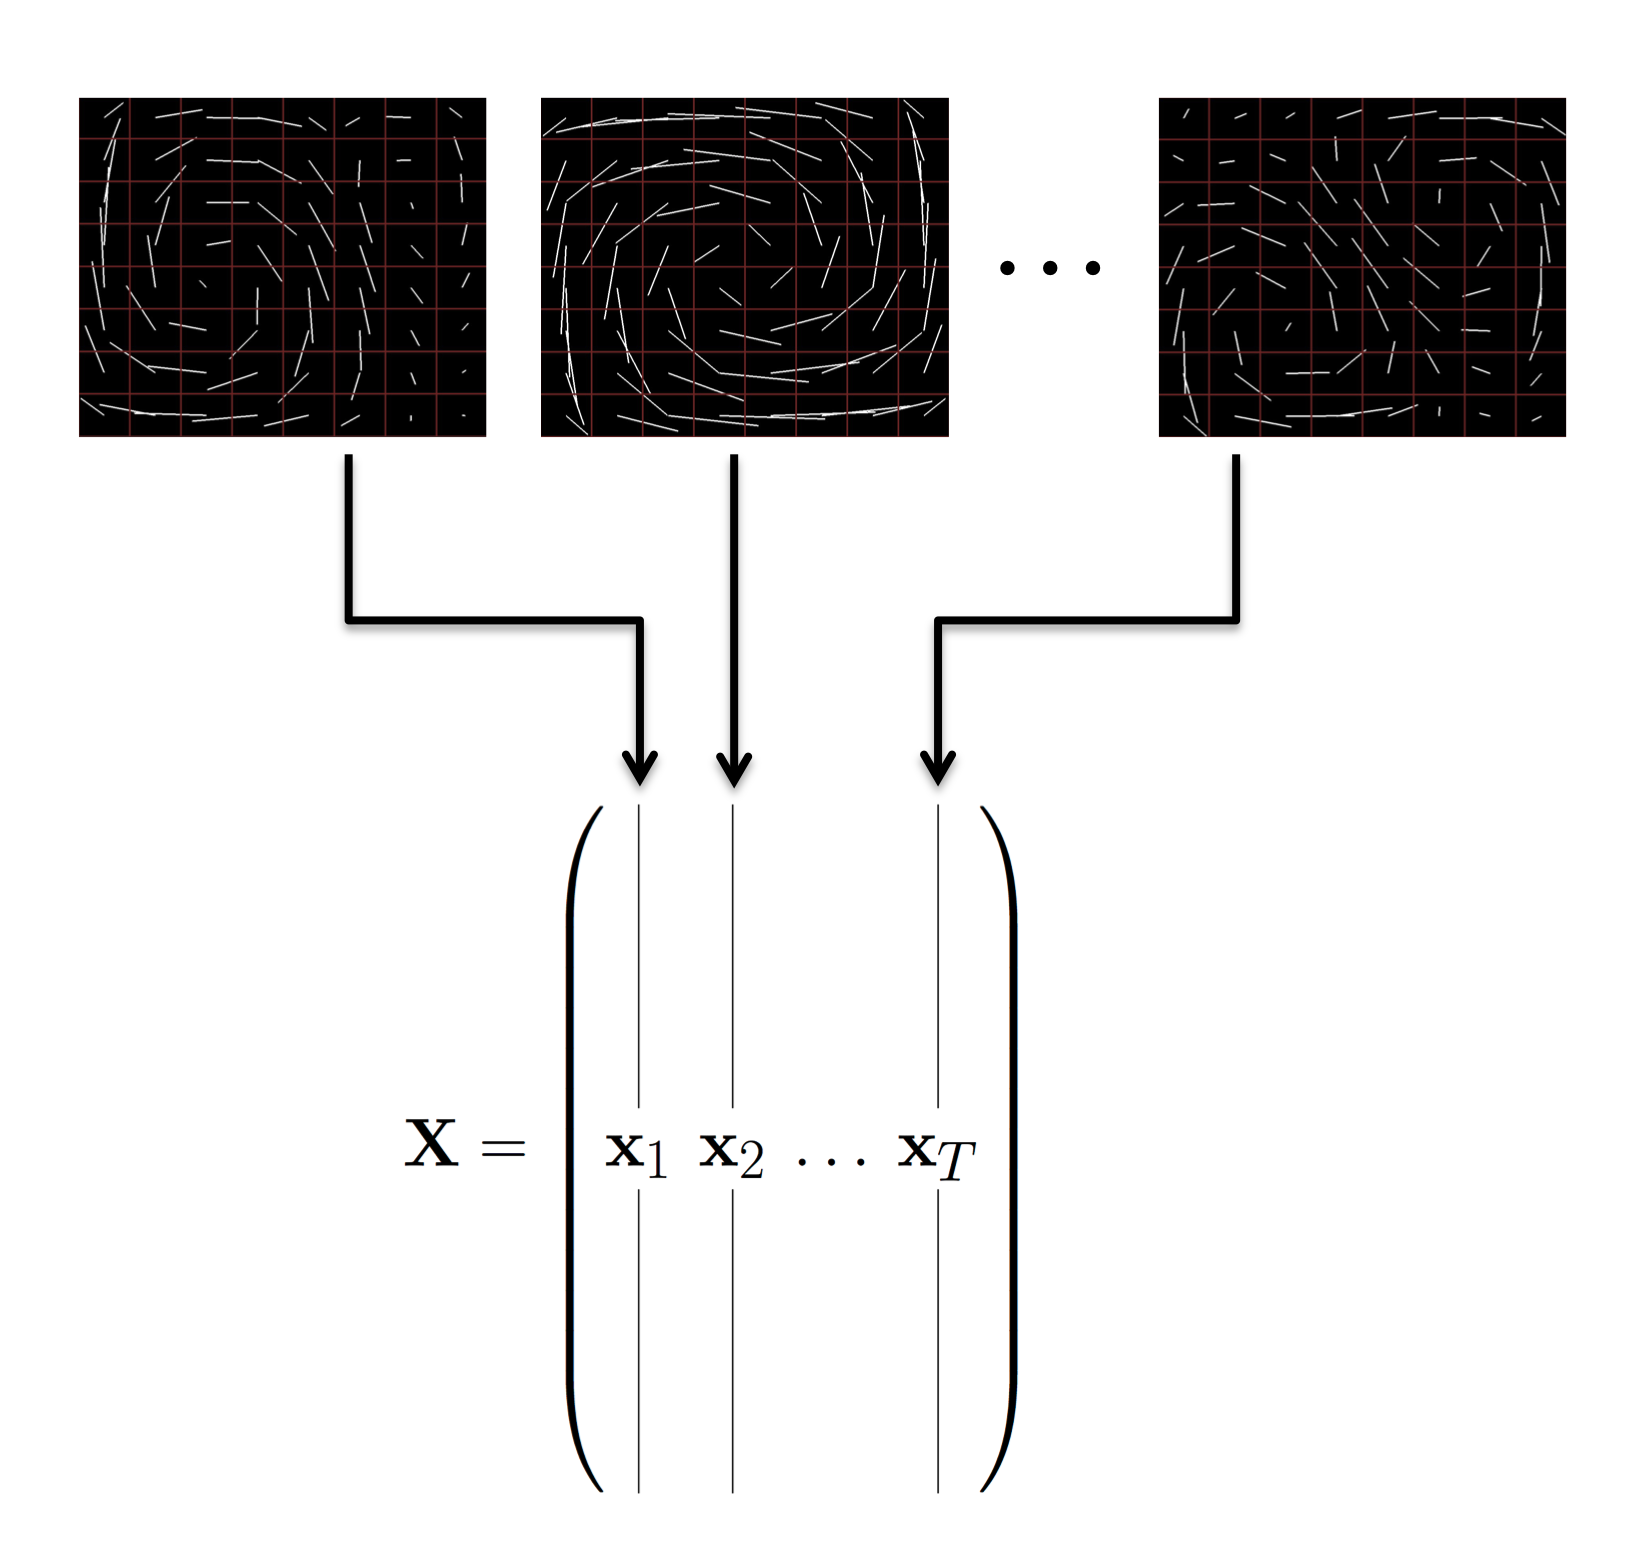
\includegraphics[height=0.45\textwidth]{Figures/assembly_matrix.png}
		%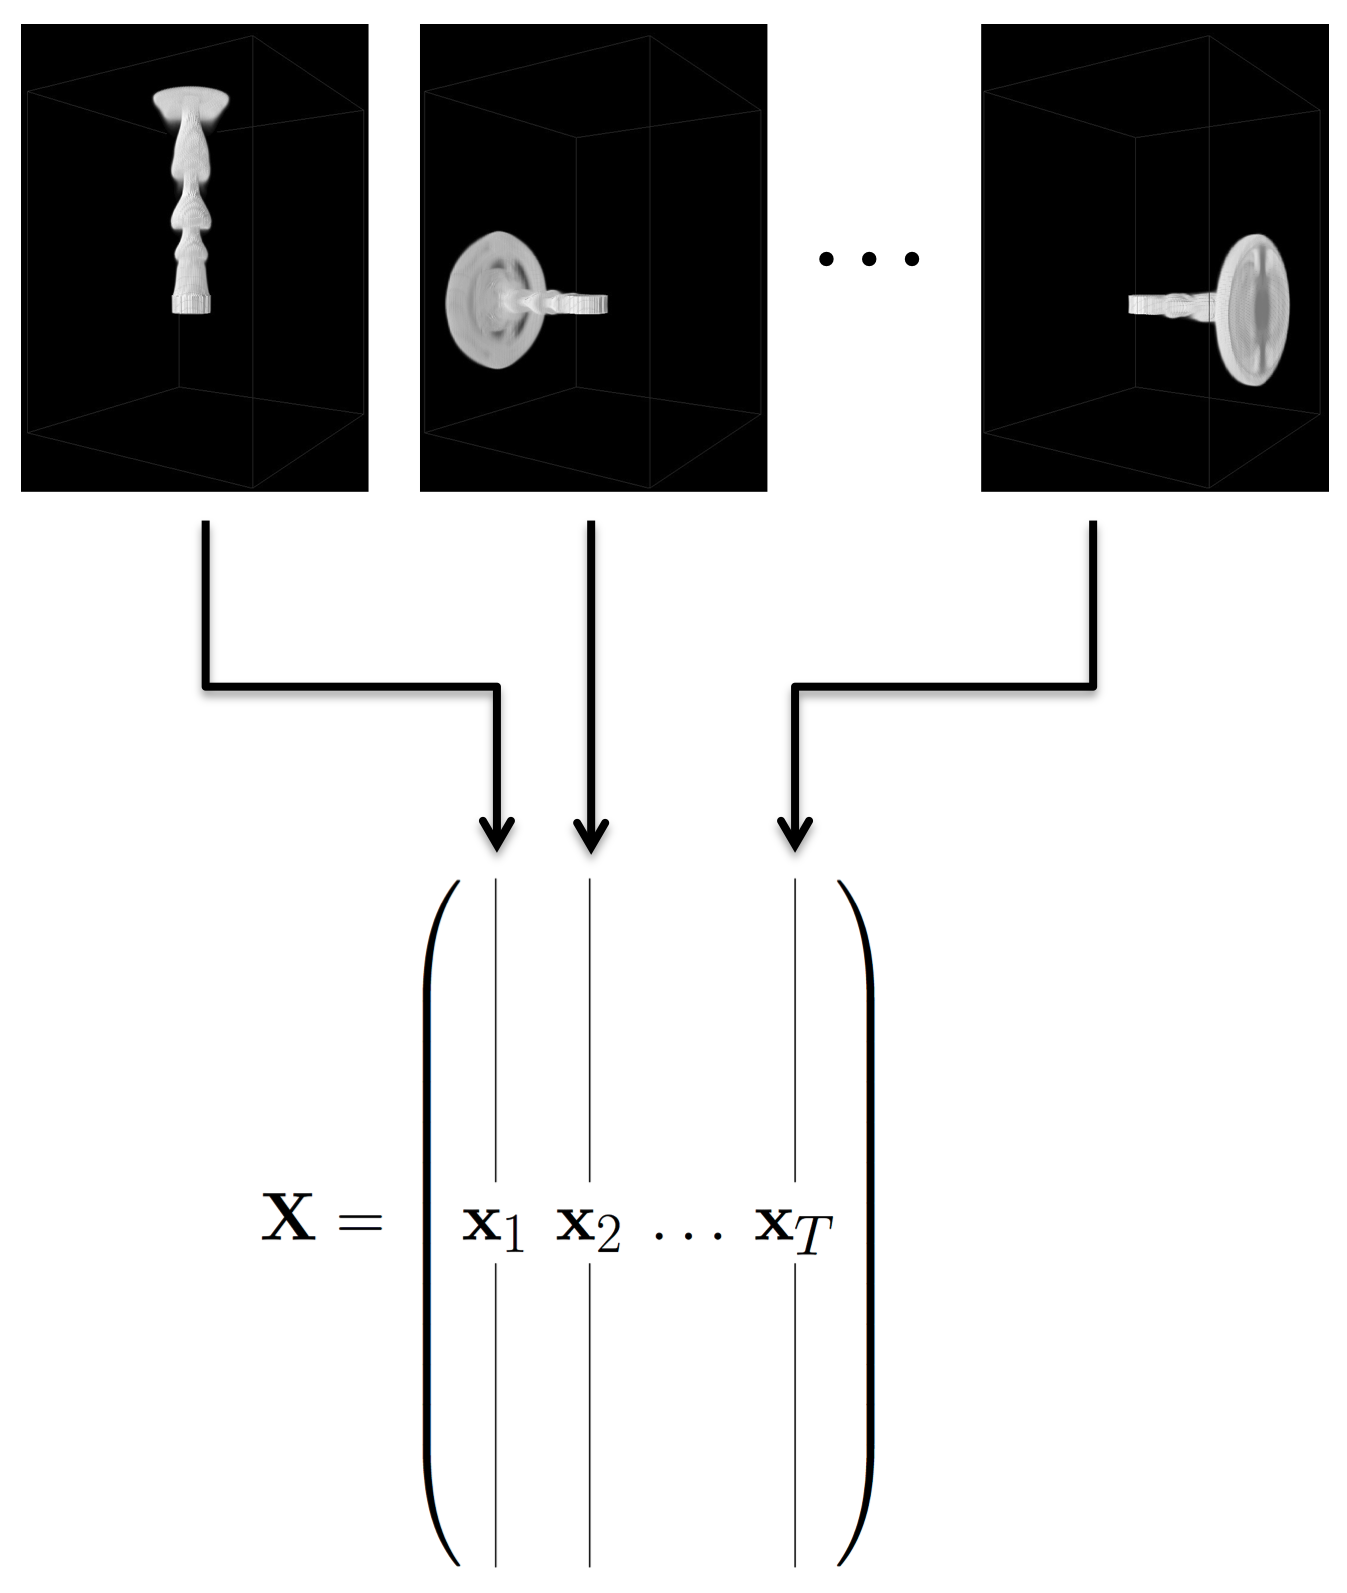
\includegraphics[height=0.45\textwidth]{Figures/plume_training.png}
		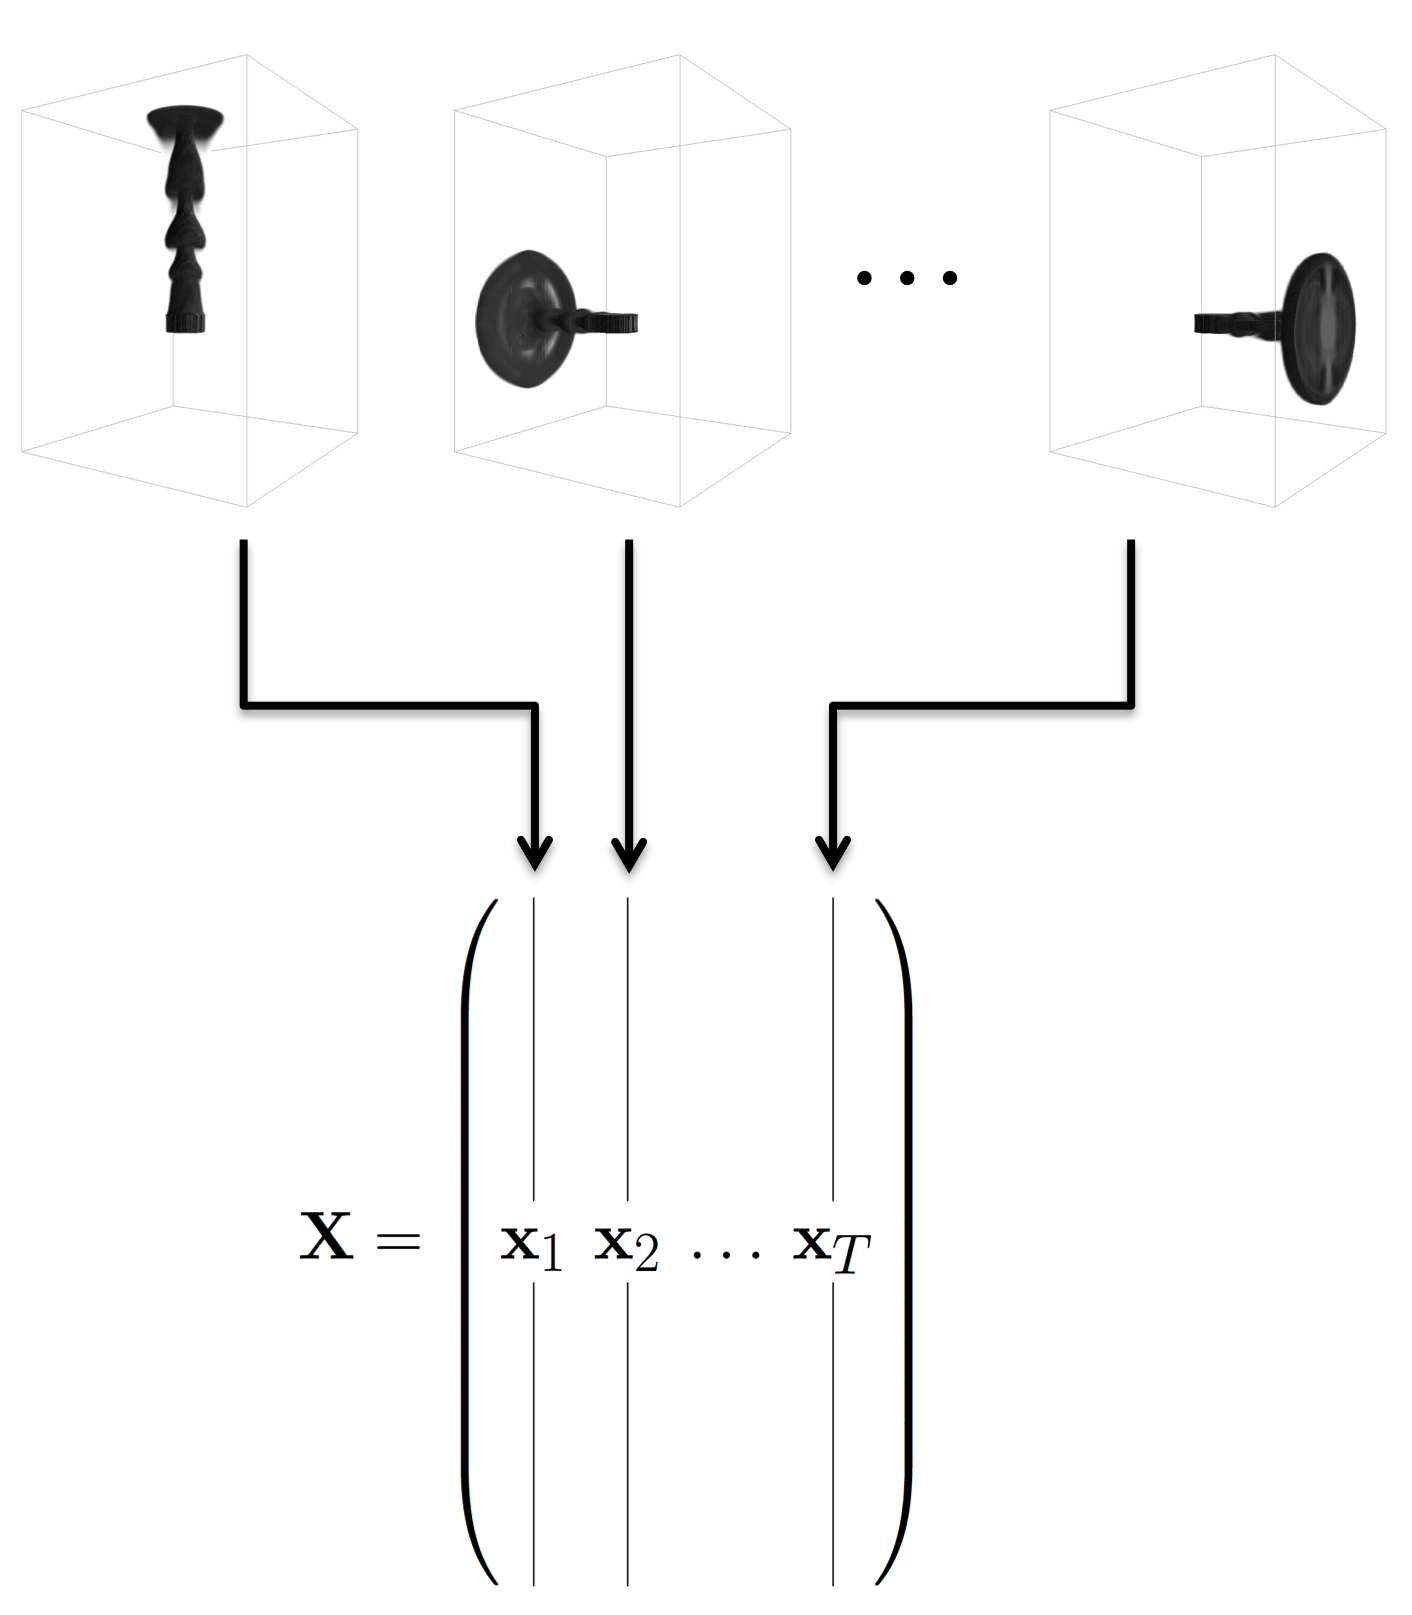
\includegraphics[height=0.45\textwidth]{chap5/figures/plume_inverted_training.png}
		%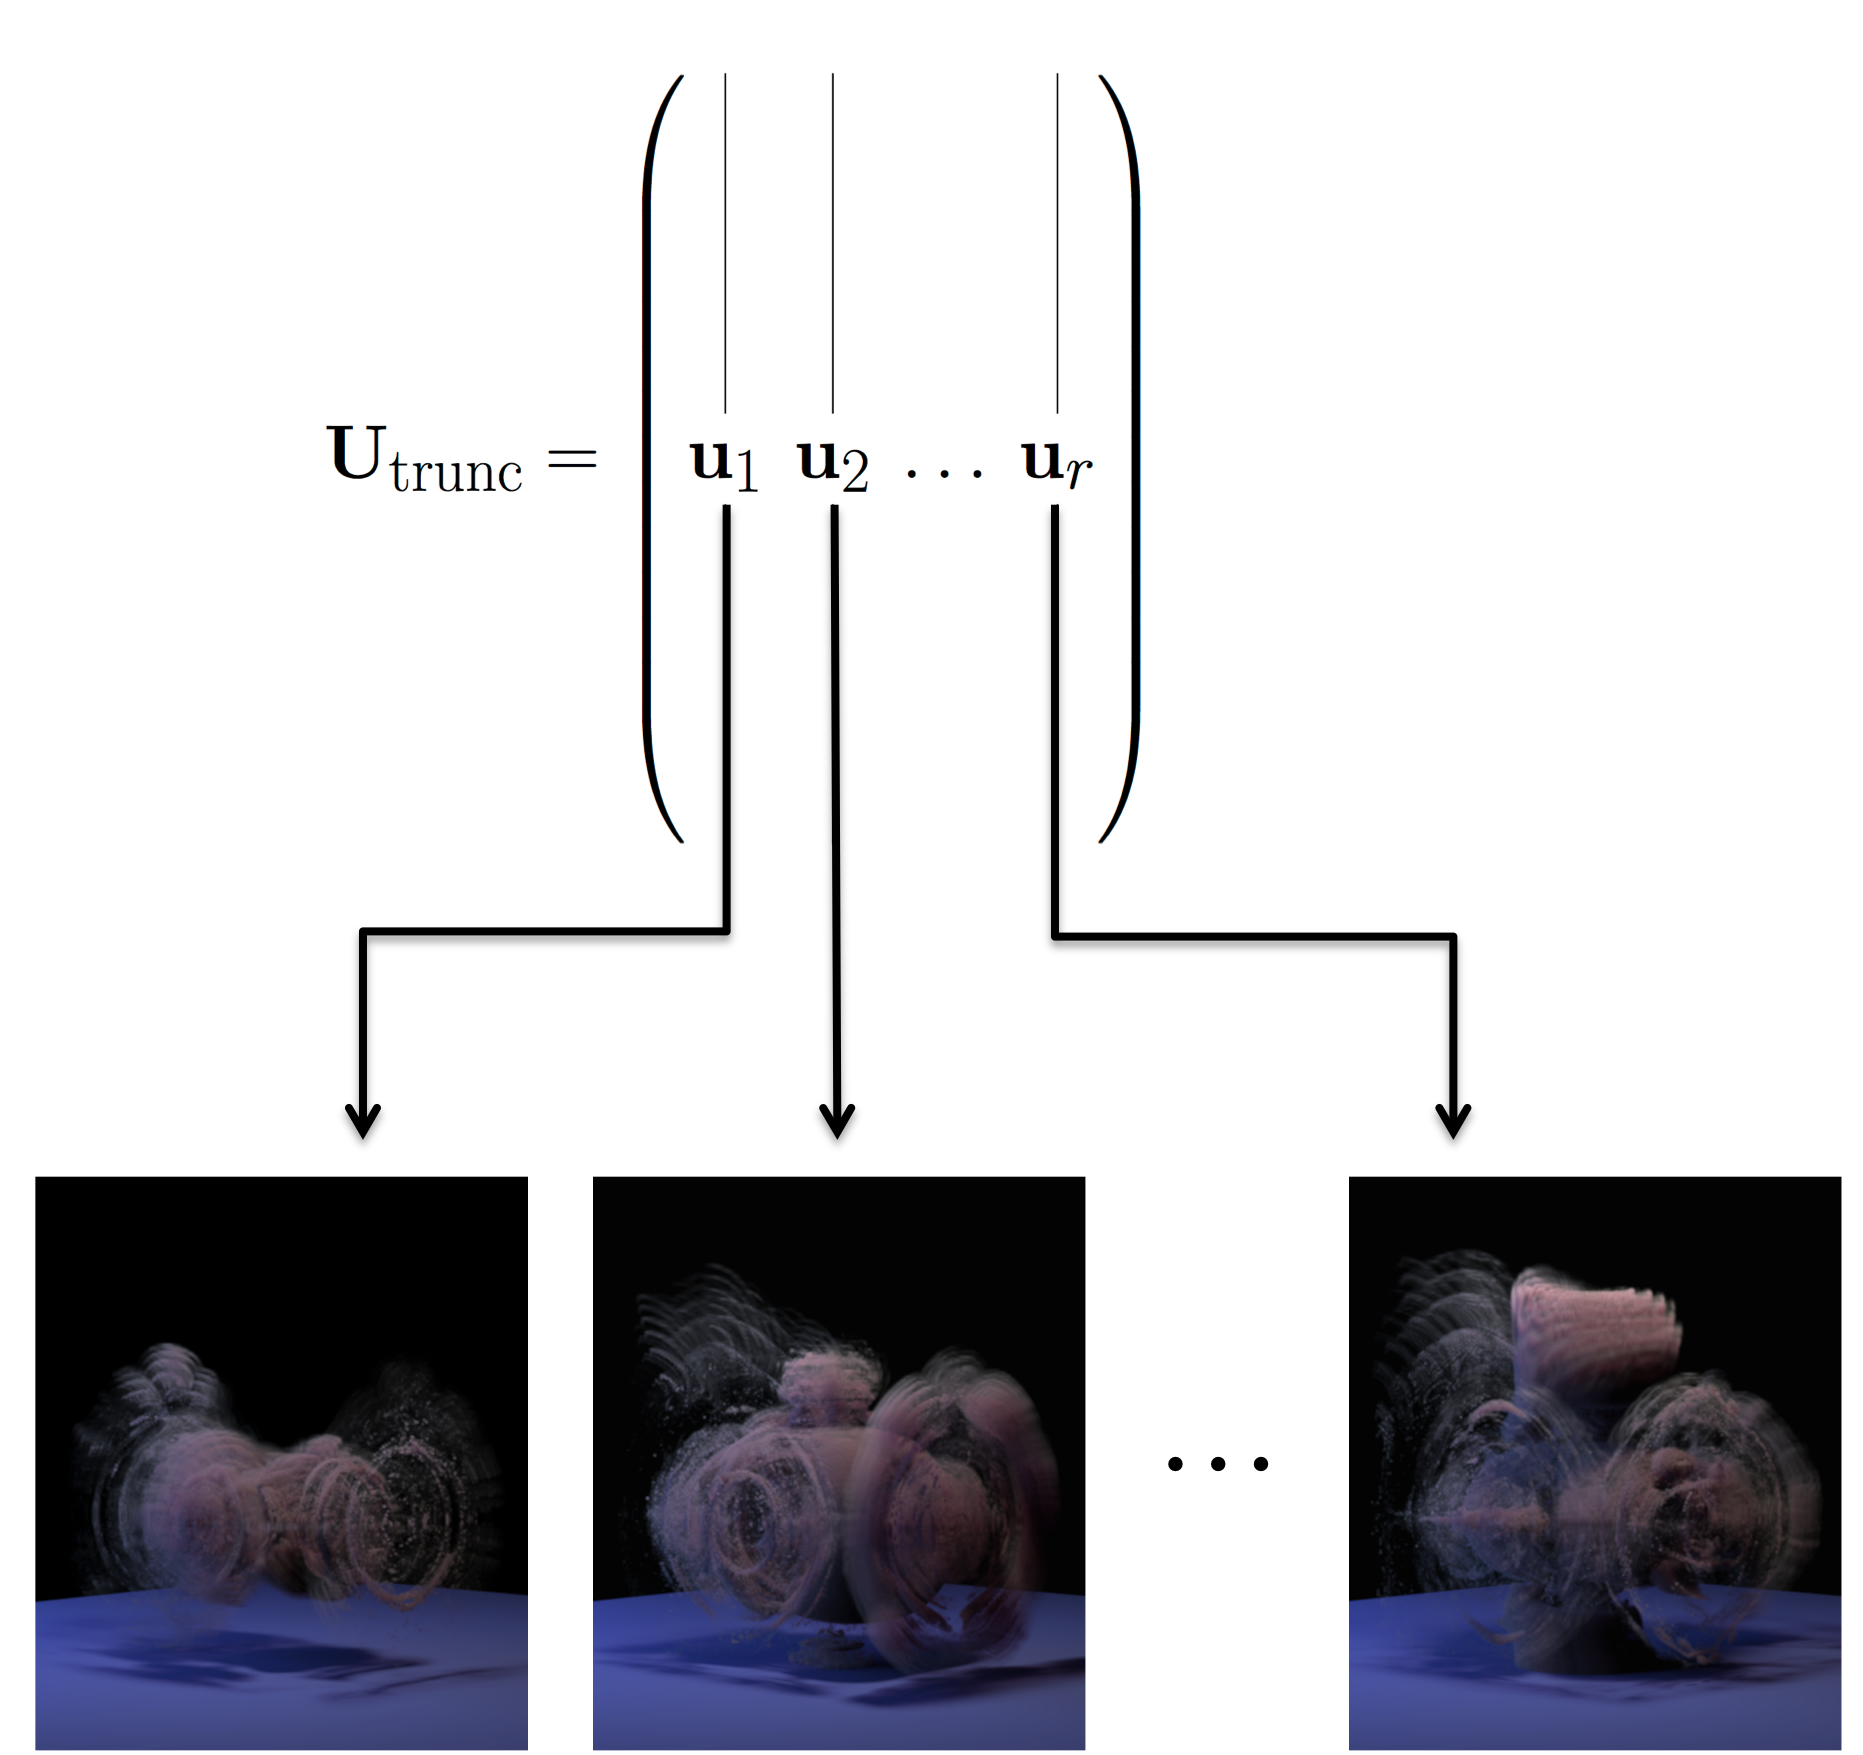
\includegraphics[height=0.45\textwidth]{Figures/U_trunc.png}
		%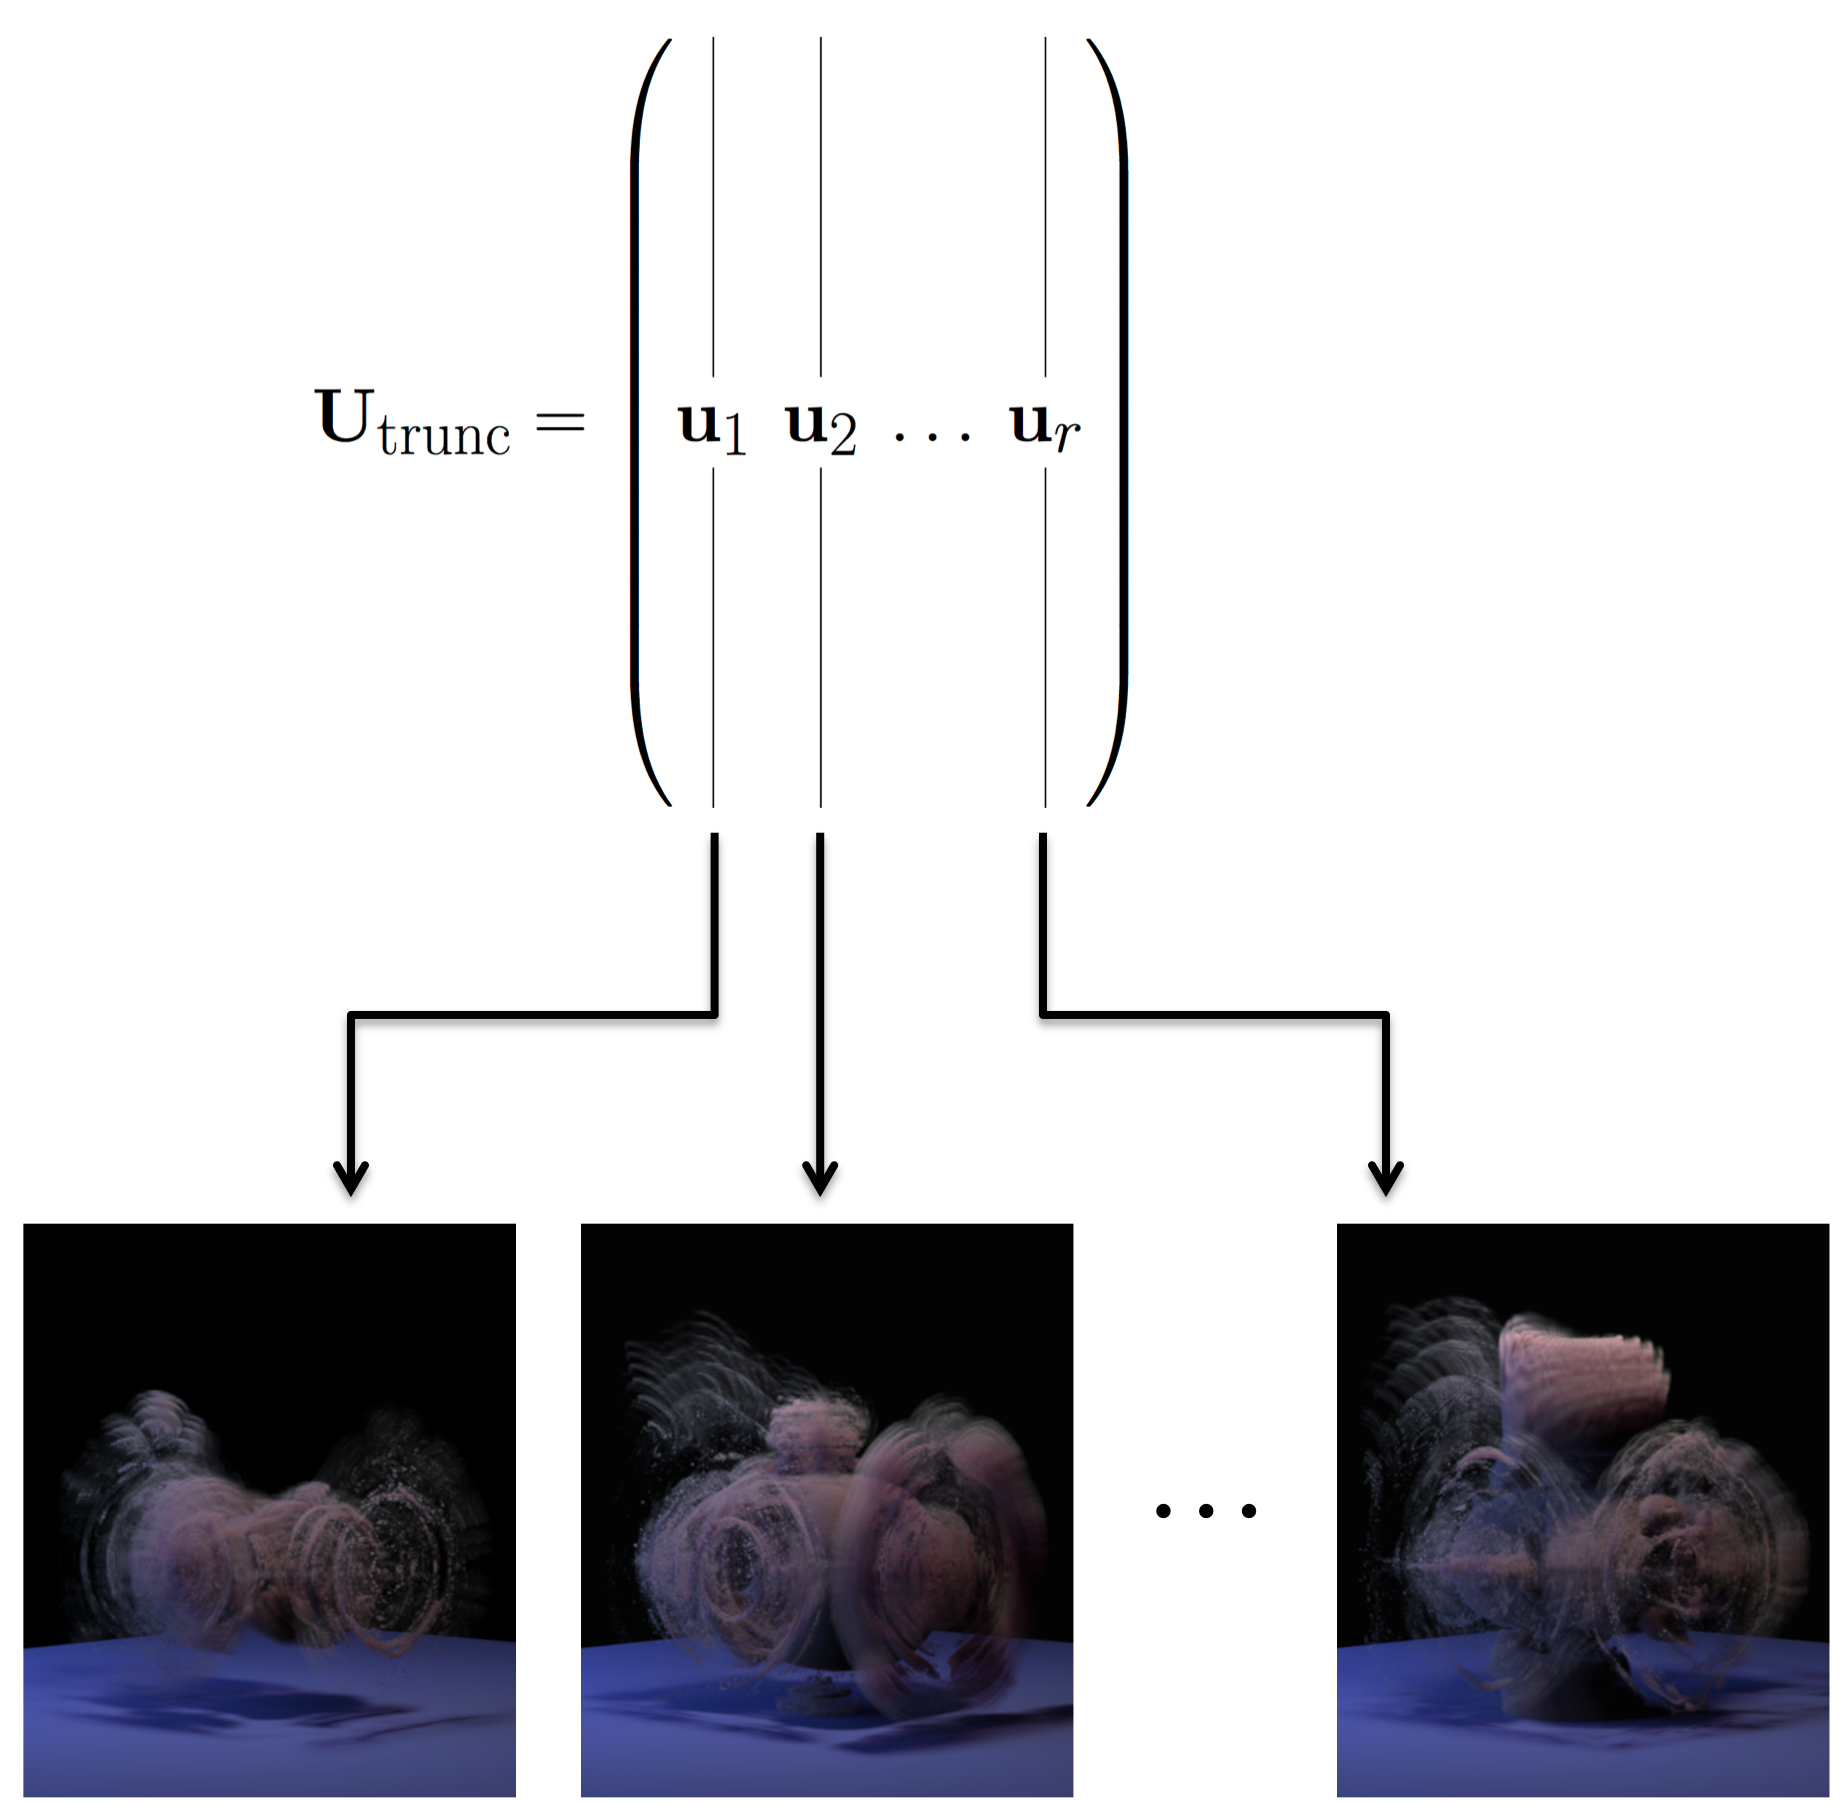
\includegraphics[height=0.45\textwidth]{Figures/U_trunc_alt.png}
		%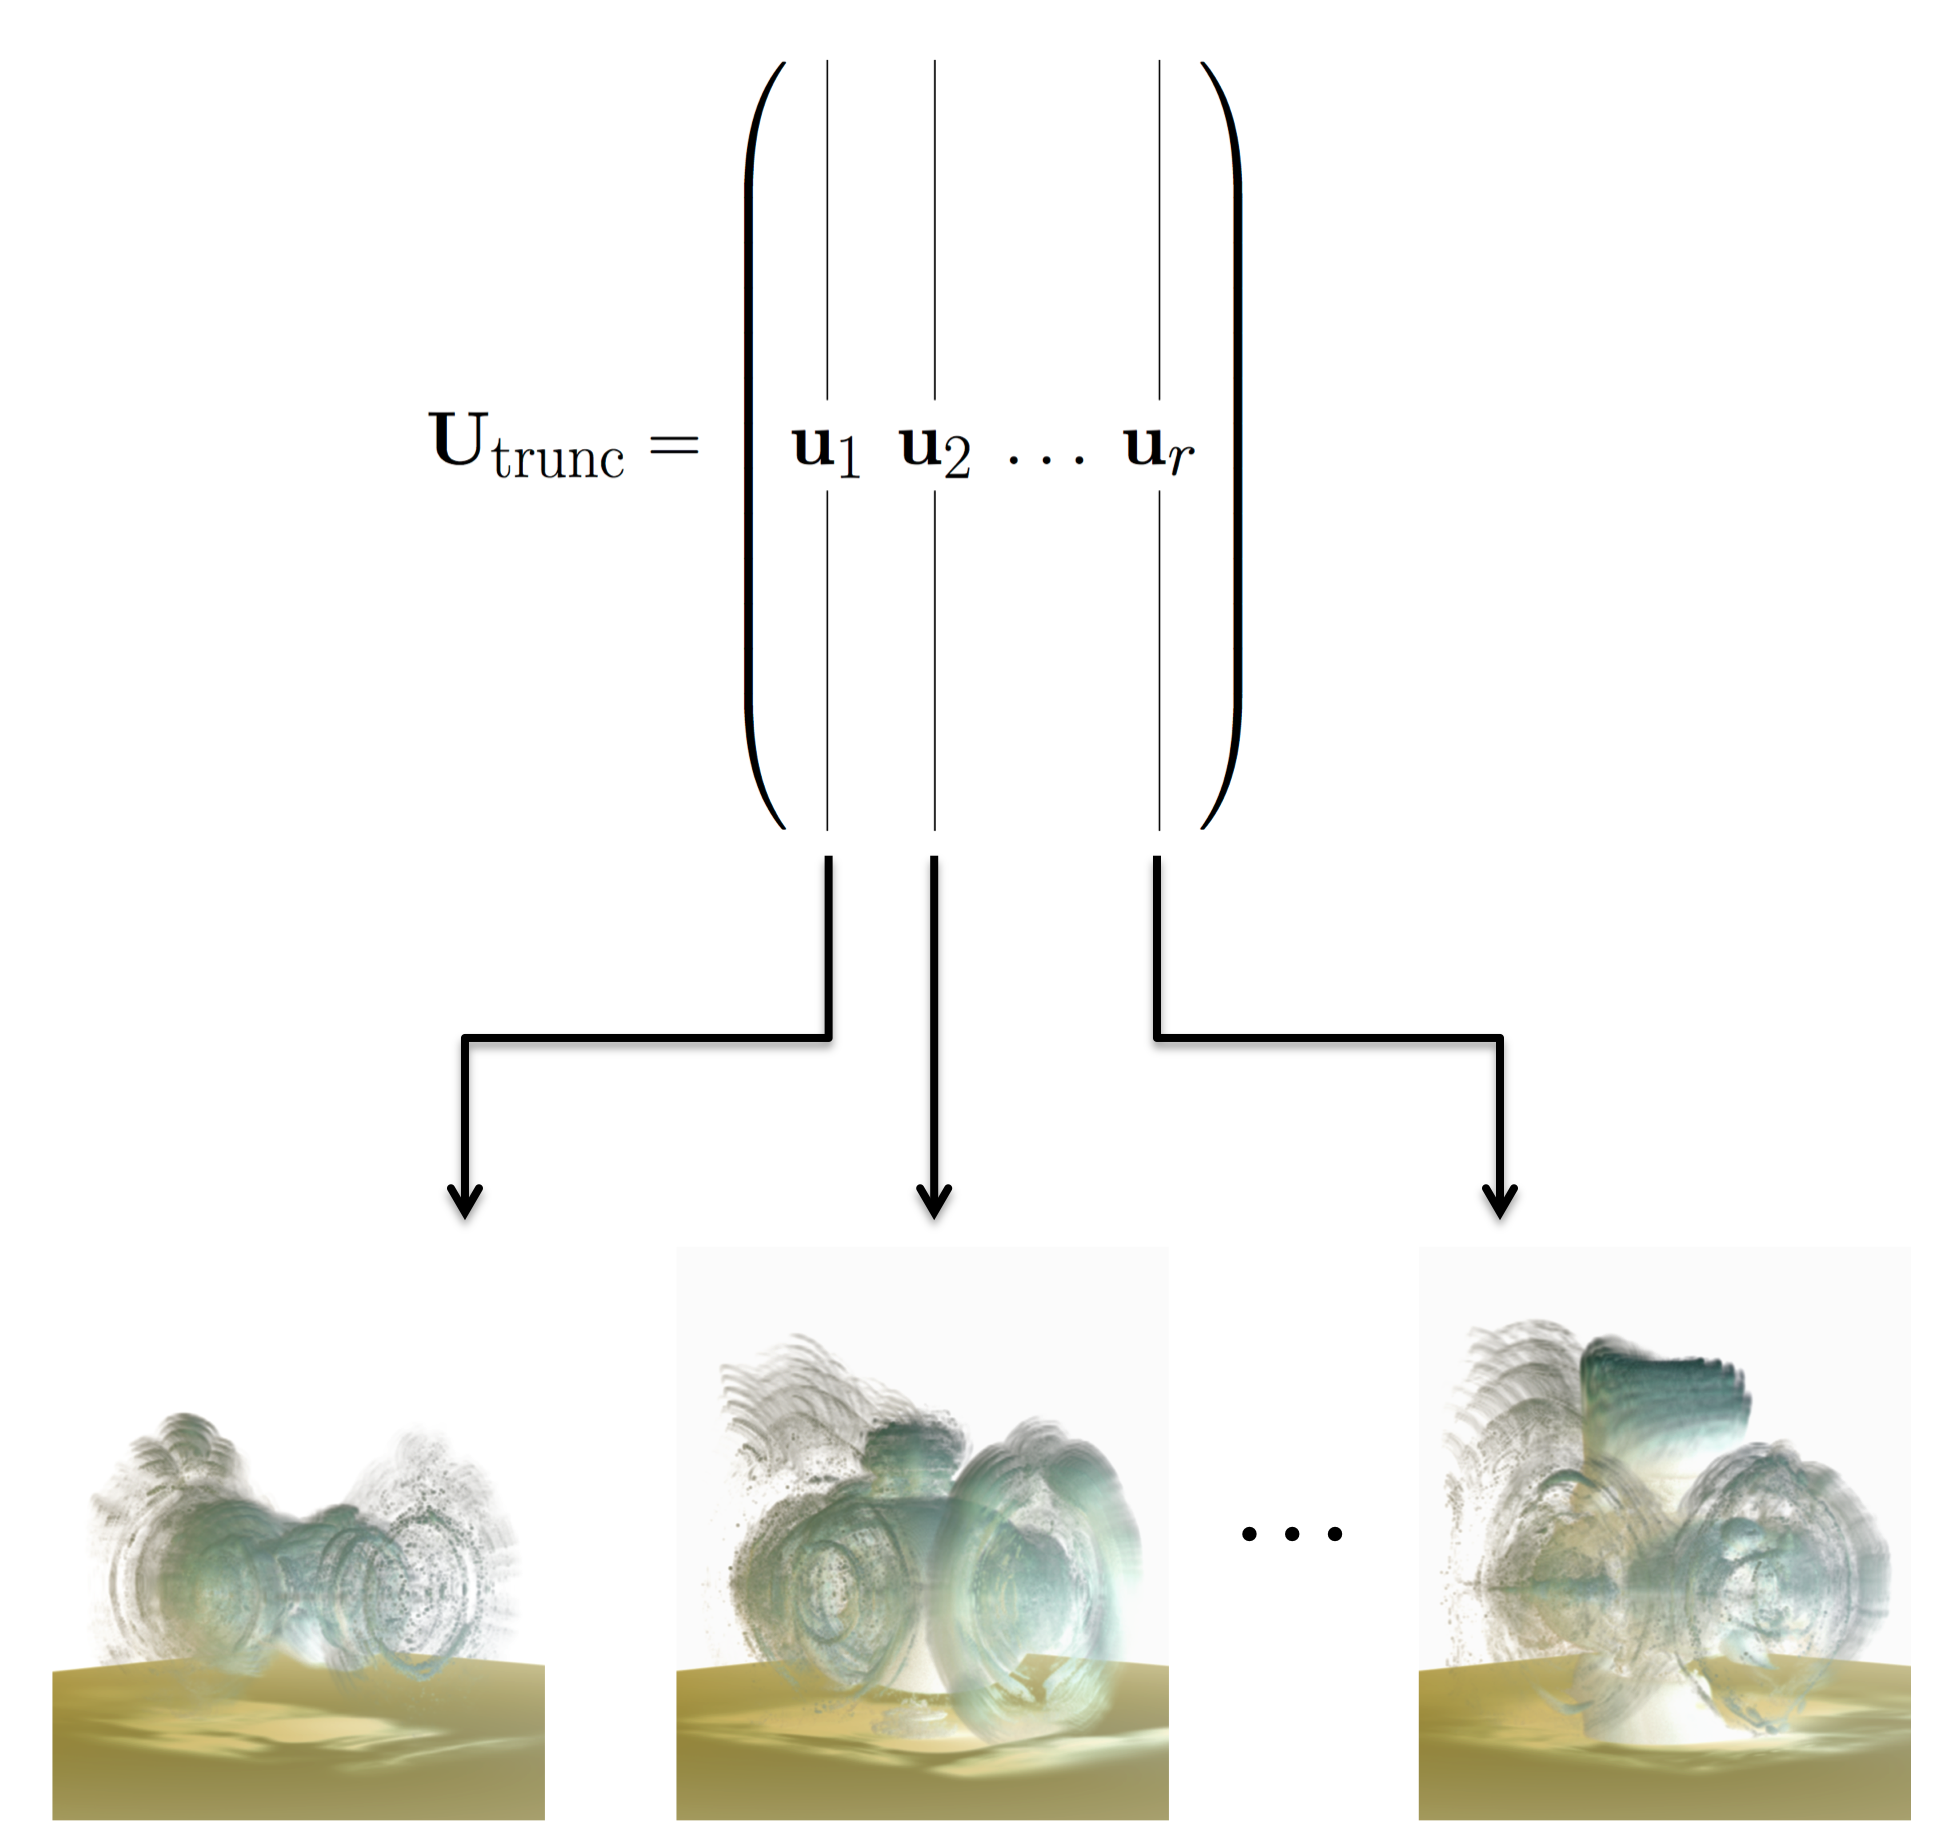
\includegraphics[height=0.45\textwidth]{Figures/U_trunc_invert.png}
		%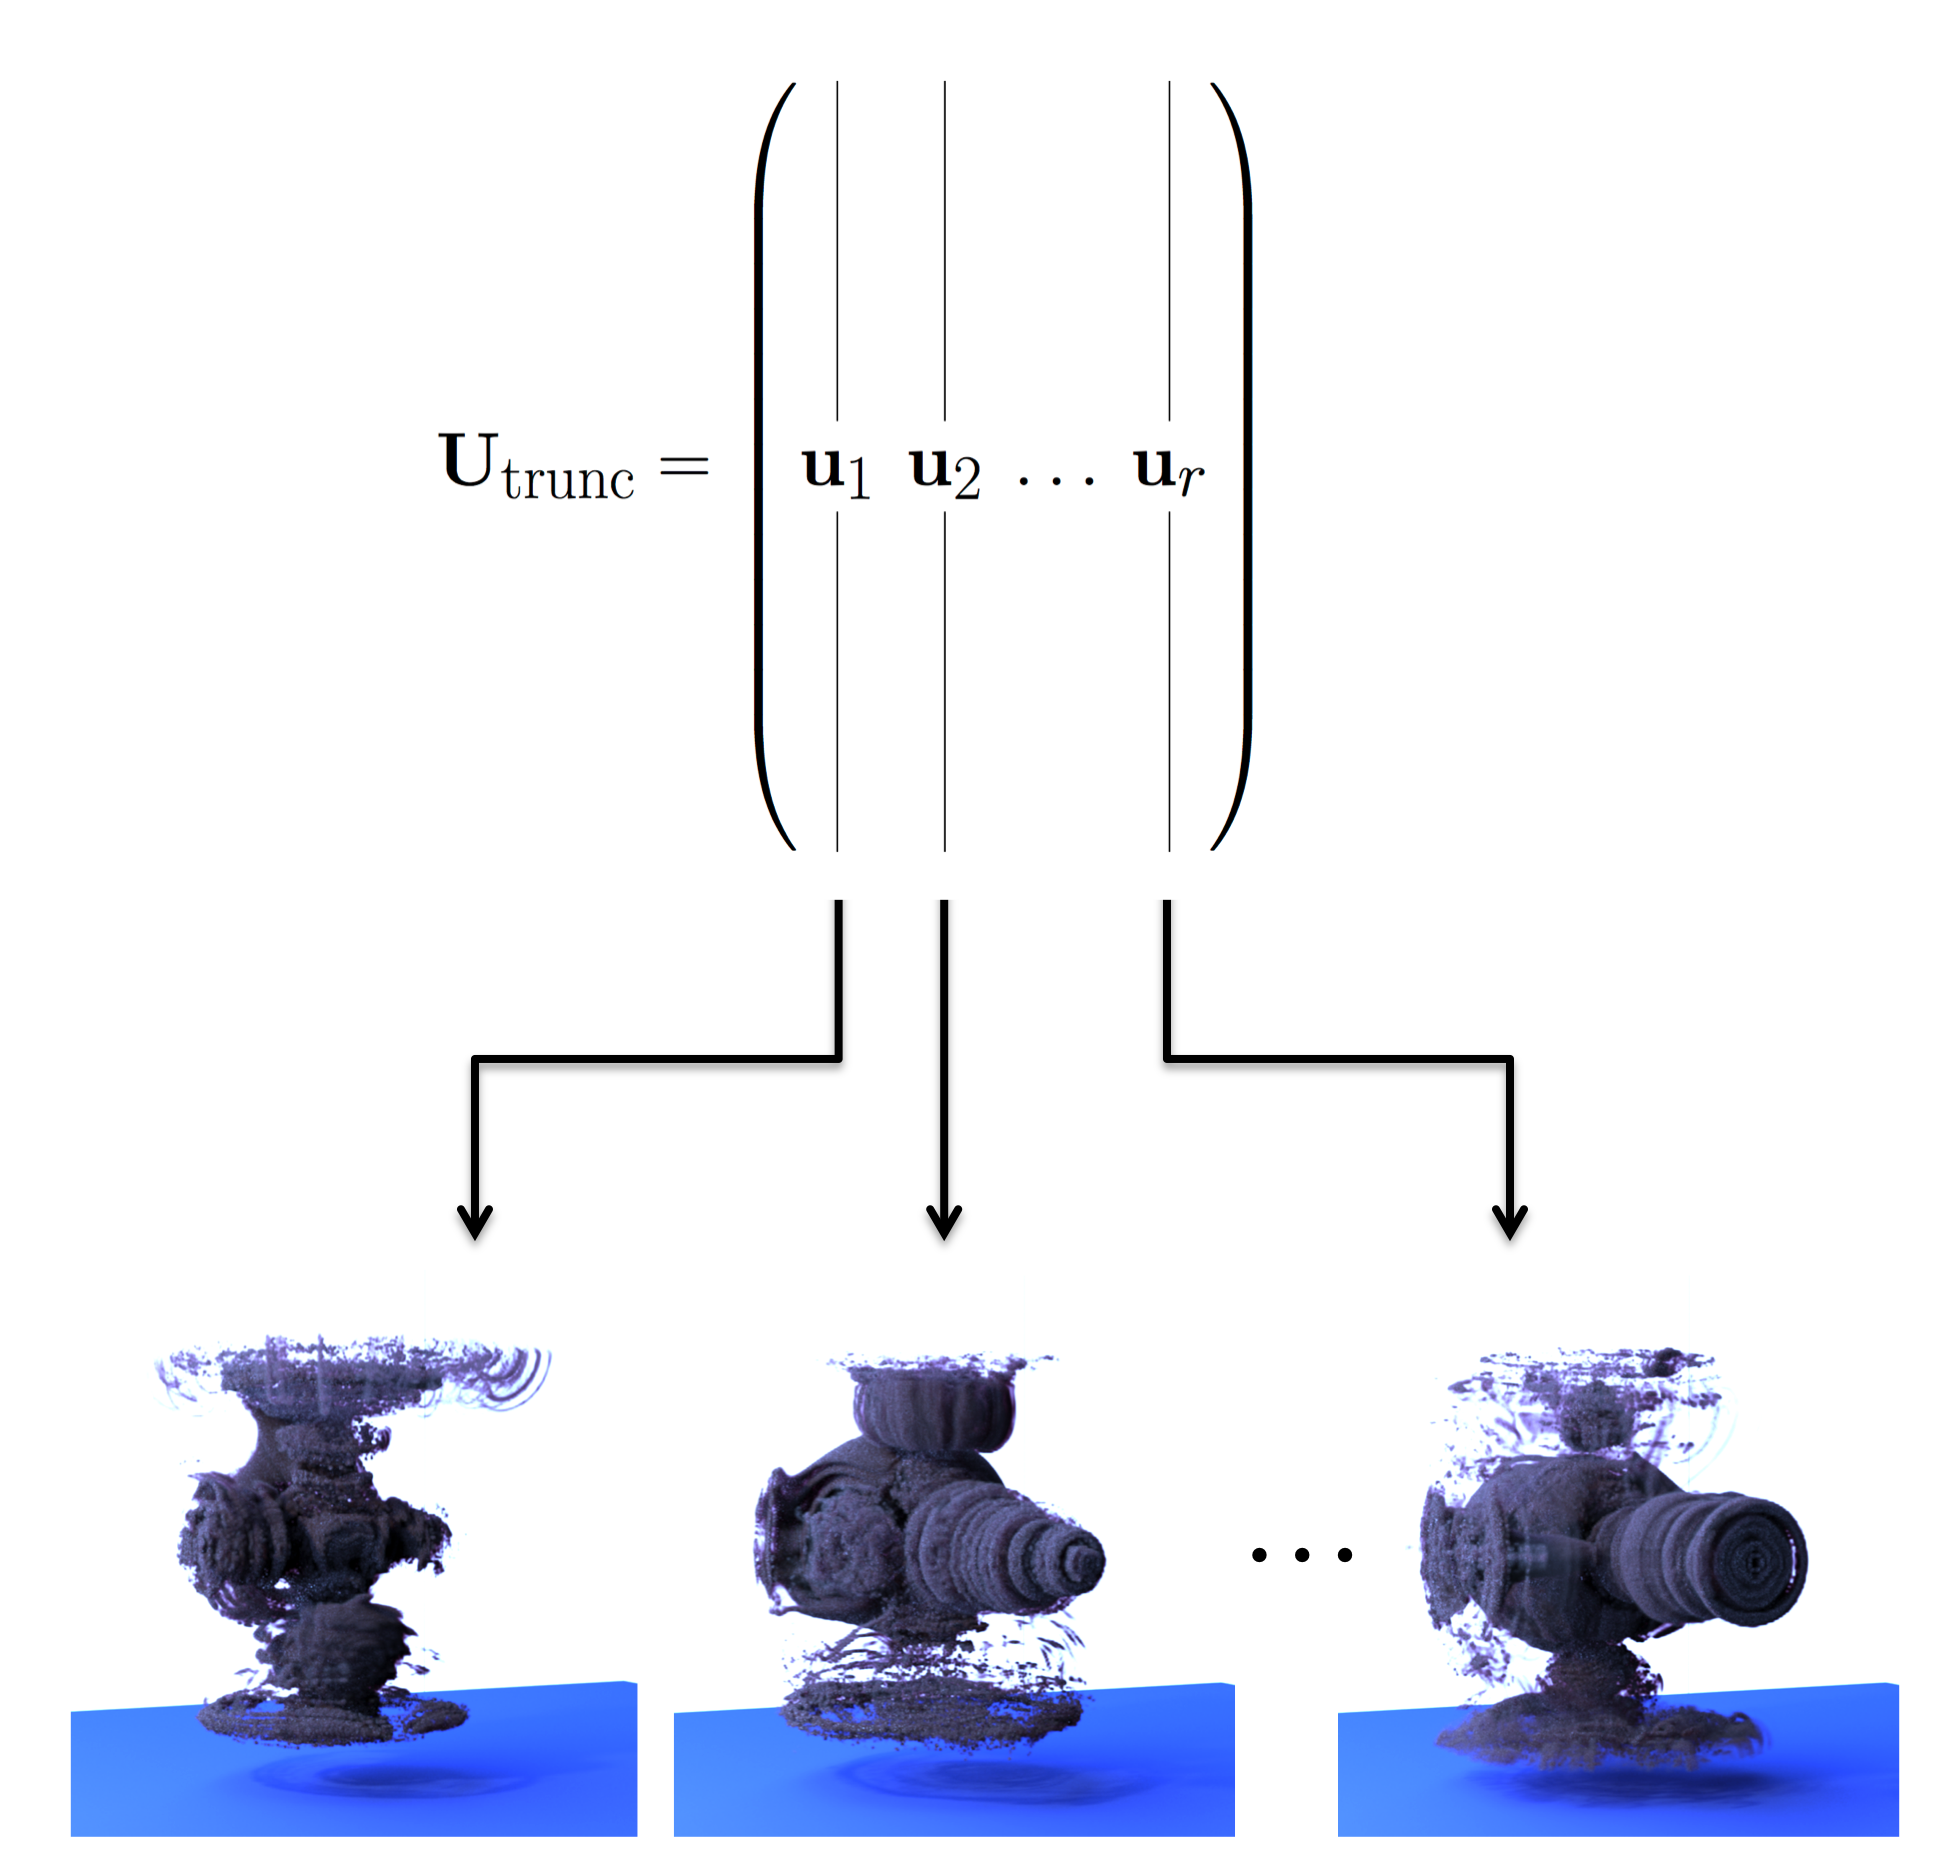
\includegraphics[height=0.45\textwidth]{Figures/U_trunc_recolored.png}
		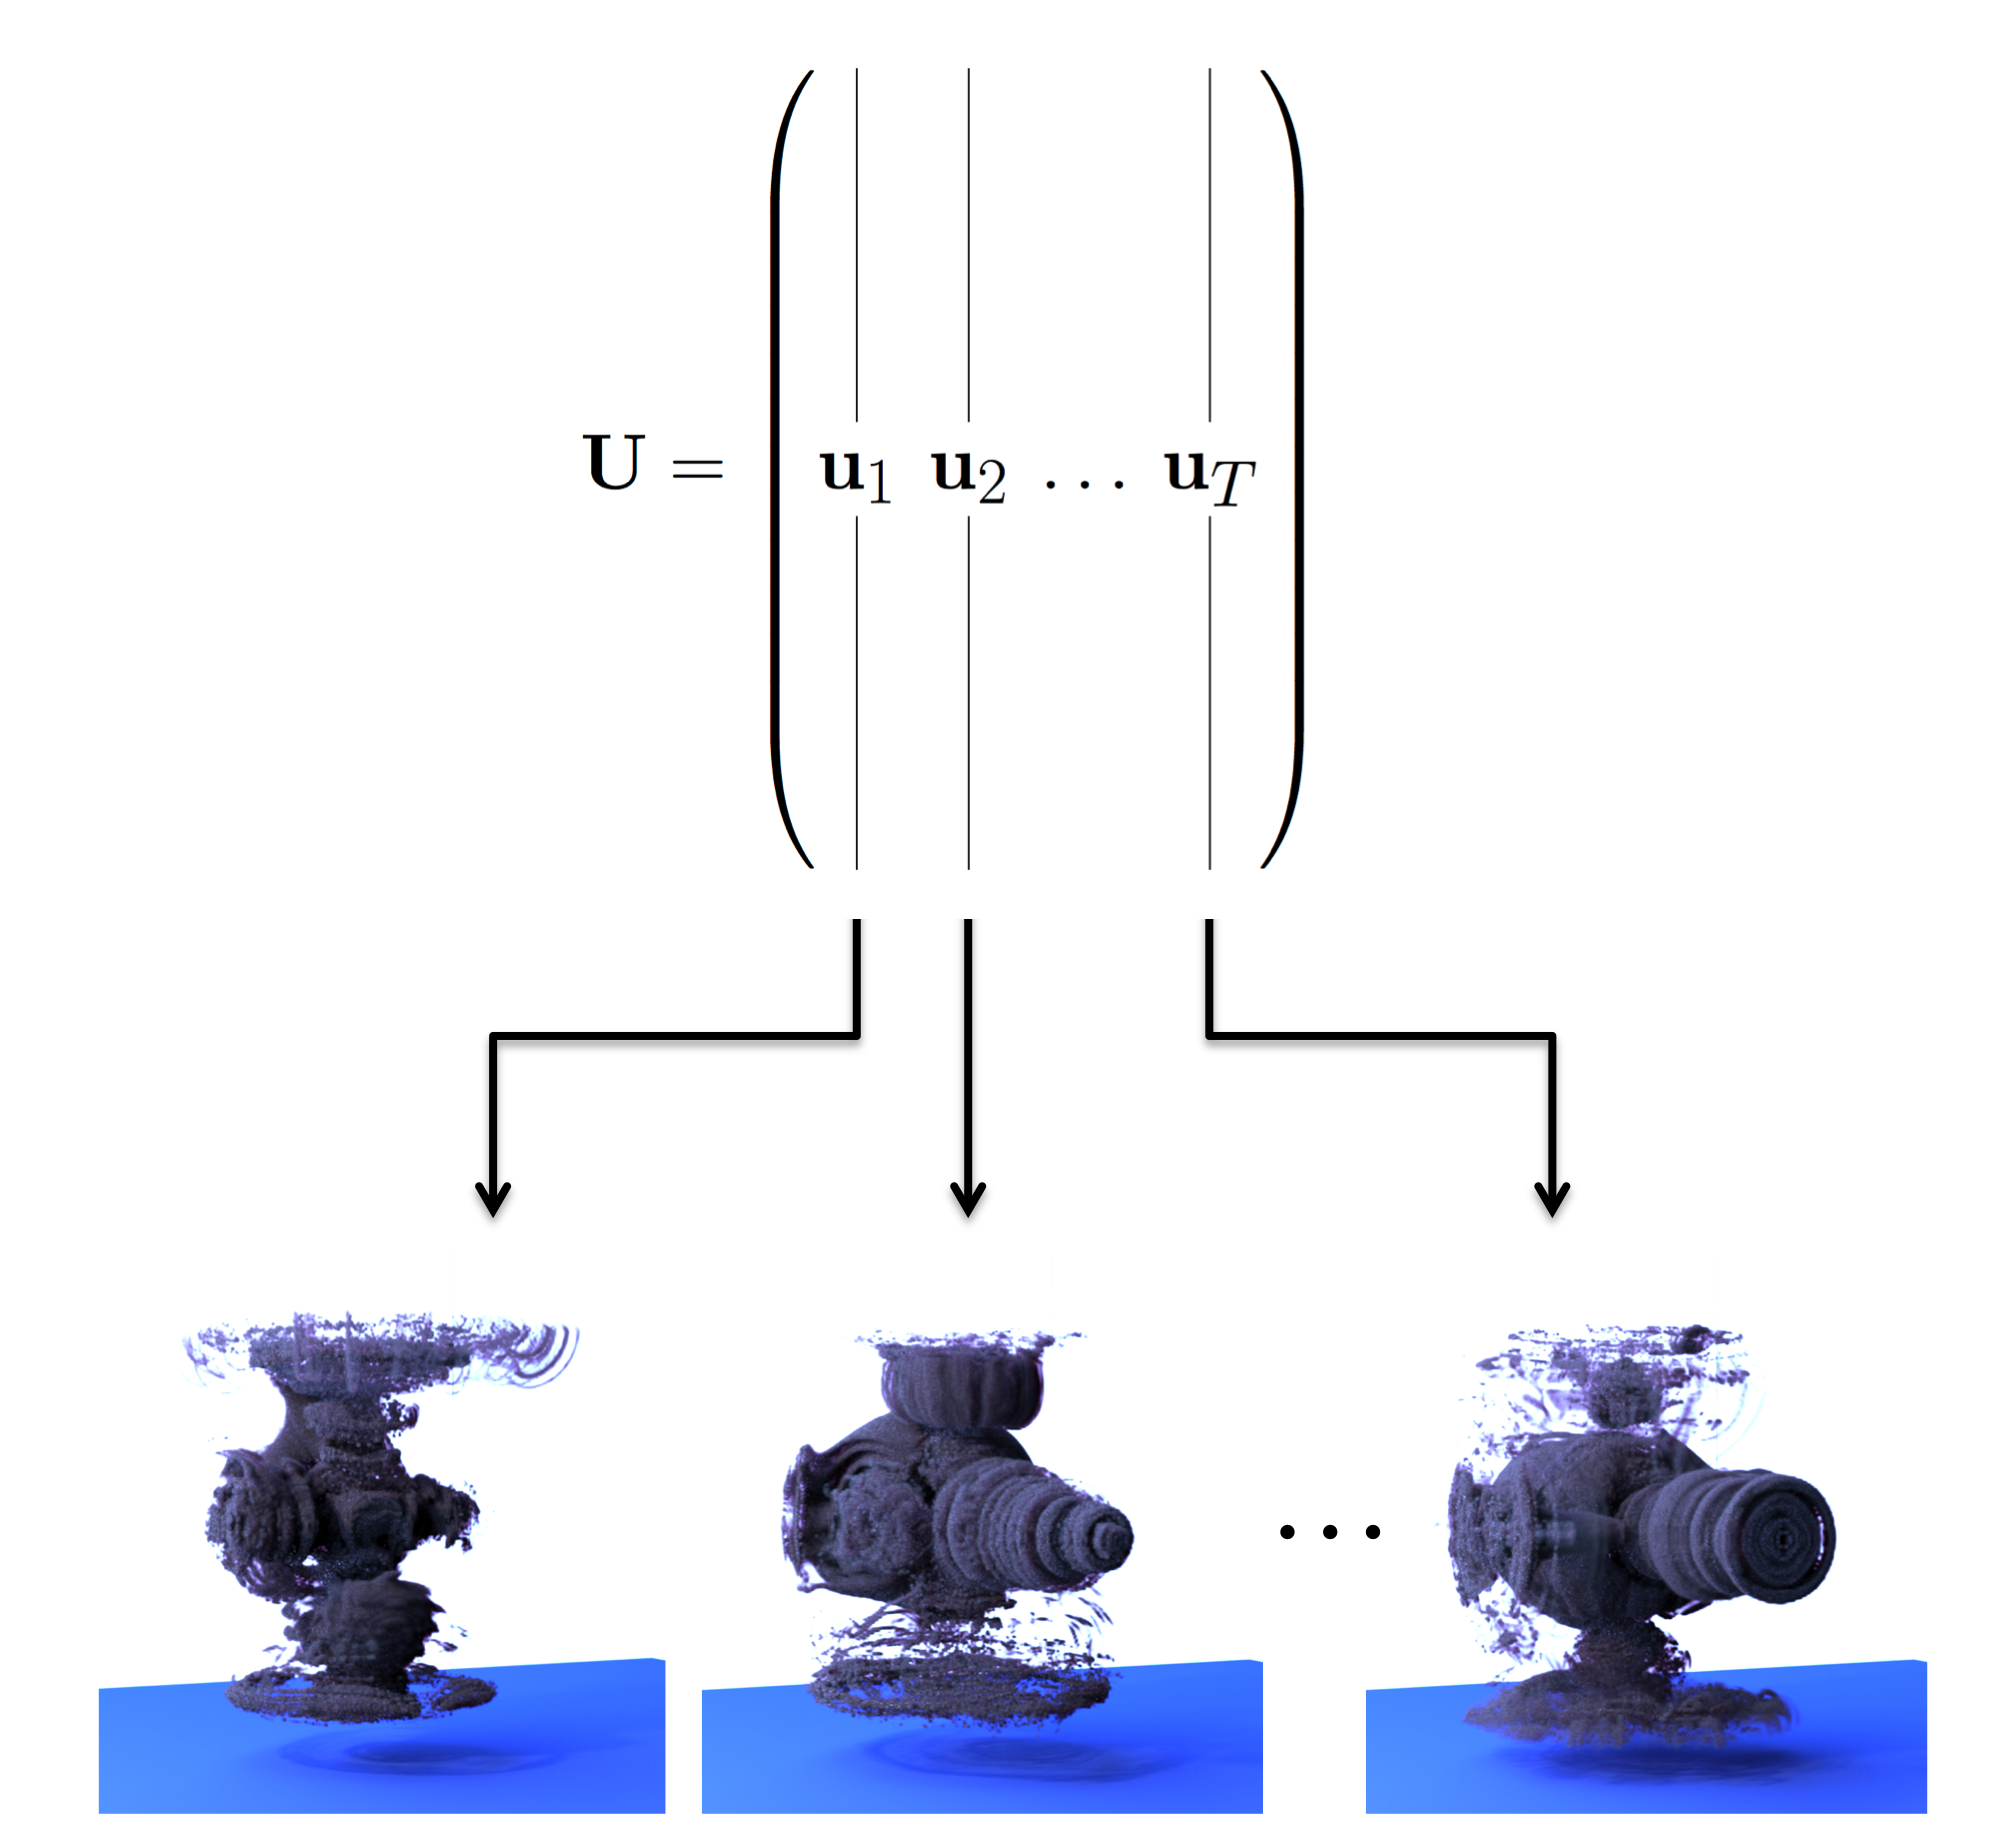
\includegraphics[height=0.45\textwidth]{chap5/figures/U_trunc_T.png}
		%		\vspace*{-1em}
		\caption{{\em{\bf Left:} Assembling the velocity fields column-wise into a matrix $\boldX$. We use simulations of a plume moving toward each face of its bounding box.}\\{\em{\bf Right:} Obtaining the empirical eigenvectors after the singular value decomposition is performed on $\boldX$, yielding $\UU$.}}
		\label{fig:matrices}
\end{figure}
\section*{Empirical Eigenvectors in Computational Fluid Dynamics}

The eigenvector analysis that automatically discovers Chladni patterns does not extend directly to more complex phenomena. Nevertheless, we are interested in discovering analogous patterns that arise in turbulent fluid flows, as they may have artistic value. The equations for these flows are inherently non-linear, while the eigenvector approach is linear, so we will instead use the method of ``empirical'' eigenvectors. In order to motivate these techniques, we will introduce some concepts from computational fluid dynamics.

A fluid is usually defined using a velocity field, where a velocity vector is associated with each point in space. While there are many different ways to represent these fields, we take the perspective from the previous section where a bounded region of space has been diced into a set of regular squares (or, in $\threeD$, cubes). Each cube is then assigned a corresponding velocity vector (Figure ~\ref{fig:velocity-field}), and in order to generate an animation, the vectors must then be evolved over time. There are many different equations that can be used to specify this evolution in time, but we use the well-known incompressible Navier-Stokes equations for fluid flow. A detailed discussion of these equations is beyond the scope of the current work. We instead assume that we have divided time into a discrete number of steps, and that at each step, the vector inside each cube in our computational grid has been assigned an appropriate value. Further details on the numerical integration methods we employ can be found in the paper by Stam \cite{Stam99}.

%We begin with a brief discussion of some fundamental techniques in computational fluid dynamics (CFD). Fluid flow is typically represented by a velocity fields, which associate a velocity vector to each point in space. For computational purposes, we regularly partition space discretely into many small cells so that each cell has an associated velocity vector (Fig.~\ref{fig:velocity-field}). To create animations, the velocity fields must also evolve over time. To that end, the incompressible Navier-Stokes equations are a well-known set of differential equations which model the time evolution of fluid flow. Although a detailed discussion of these equations is beyond the scope of the current work, on a high level, assuming we have a computational approximation to these equations, this means we can subdivide time into discrete timesteps and simulate the evolution of each velocity vector in each cell as it changes from one timestep to the next. 



Unlike the classic Chladni pattern case, CFD simulations do not yield a single matrix $\boldA$ on which an eigenvalue analysis can be performed. The non-linear operations involved generate a new, time-dependent matrix $\boldA$ at every timestep. Instead of one canonical $\boldA$ that can be said to characterize the behavior of the entire system, there are instead infinitely many $\boldA$s, none of which inherently take precedence over the others. Fortunately, if some sort of precedence is imposed, a process akin to an eigenvalue analysis can still be applied.
The method of ``empirical'' eigenvectors \cite{Ryckelynck2005}, also known as the Proper Orthogonal Decomposition, Karhunen-Love expansion, or Hotelling transform, establishes one such criterion. Informally, given an existing simulation, we can analyze the series of matrices that arose during that simulation and give those matrices precedence over all others. The space of infinite $\boldA$s is thus reduced to a tractable, finite size.

%\section*{Empirical Eigenvectors of a Fluid}
%In this section, we would like to discover a characteristic set of velocity fields that can be combined to generate a wide range of fluid motions. Given a particular mathematical operator, we can study its eigenvectors, or characteristic vectors. These vectors, loosely speaking, are the inputs to the operator that transform by scaling only. Eigenvectors are especially useful if we can describe arbitrary inputs to the operator as a mixture of eigenvectors, since this allows us to easily compute the outputs.

%In our work, the operator in question is the Navier-Stokes equations for fluid flow. There are several different strategies for computing the eigenvectors associated with this operator. For example, de Witt et al. \cite{deWitt:2012} computed the analytic eigenfunctions of the fluid velocity field over a simple square domain, and used them to advect (i.e.~push) a particulate through space. These eigenfunctions are composed of separable products of sines and cosines, and the results visually correspond closely to classic Chladni patterns (Fig.~\ref{fig:chladni-plate}, right).

%We are interested in generating less classical results, so we prefer the use of ``empirical'' eigenvectors~\cite{Ryckelynck2005}. This approach goes by many names, such as the Proper Orthogonal Decomposition, Karhunen-Love expansion, or Hotelling transform, but we prefer the eigenvector nomenclature because it clarifies the connection to Chladni patterns. As the name suggests, it involves computing the eigenvectors of an empirically obtained data set, which in this case is the results of a CFD simulation.

Returning to Figure \ref{fig:velocity-field}, we first perform a simulation over a regular $N \times N$ grid for $T$ timesteps. While the simulations in our actual experiments were run in $\threeD$ (Figure \ref{fig:eigs}), we will limit our discussion to $\twoD$ for simplicity. Each grid cell then contains a $\twoD$ velocity vector which possesses an $x$ and $y$ component, so the entire grid contains $N \times N = N^2$ such vectors. We can rearrange these values so that they are packed into a $\oneD$ vector $\xx$, which then has $2N^2$ entries. We can perform this repacking for each of the $T$ velocity fields from the simulation and concatenate all of the vectors into a matrix $\boldX$ with $2N^2$ rows and $T$ columns (Figure \ref{fig:matrices}, left).

Generally, $2N^2 \neq T$, so the matrix $\boldX$ will be rectangular, and an eigenvalue analysis can only be performed on square matrices. However, the singular value decomposition (SVD) can always be performed regardless of dimension, and the results possess many eigenvalue-like qualities. Instead of the eigendecomposition $\boldA = \boldQ \Lambda \boldQ^T$, the SVD instead yields $\boldX = \UU \Sigma \VV^T$. Similar to the eigendecomposition, the middle matrix $\Sigma$ is diagonal, and its entries correspond to the ``singular'' values of the matrix $\boldX$. Again, similar to the eigenvalue case, the columns of the left matrix $\UU$ form an ordered set of the most important shapes, or quasi-vibration modes, that appeared during the simulation (Figure \ref{fig:matrices}, right). The matrix $\VV$ is a $T$-dimensional rotation matrix that was applied to $\boldX$ in order to arrive at $\UU$ and $\Sigma$; for our purposes, it can be discarded.

%Recall from the previous section that our simulation of velocity fields discretizes both space and time. Hence, suppose we have $N$ grid cells and $T$ timesteps. Each particular velocity field at any given timestep can be described by $N$ velocity vectors, one for each cell. In a $3\textnormal{D}$ simulation, this is a list of $3N$ numbers, which we can simply regard as a vector $\xx \in \R^{3N}$. If we assemble these vectors column-wise into a matrix, one for each timestep, we obtain a matrix $\boldX \in \R^{3N \times T}$ (Fig.~\ref{fig:matrices}, left). This construction will allow us to use matrix analysis tools on our simulation---in particular, the singular value decomposition (SVD). Roughly speaking, the SVD discovers a natural set of basis vectors that efficiently characterize the space of desired transformations determined by $\boldX$. More concretely, we obtain a factorization $\boldX = \UU \Sigma \VV^T$, where $\UU$ comprises the basis vectors of interest, $\Sigma$ comprises the associated singular values, which are scalars that determine the relative importance of each basis vector, and $\VV^T$ comprises the right singular vectors, which are discarded for our purposes.


	
%In our situation, the columns of $\UU$ are linearly independent and sorted by how well they characterize the data in $\boldX$. These columns comprise our empirical eigenvectors. Since the data in $\boldX$ is a series of fluid velocity fields, these empirical eigenvectors are the characteristic fluid velocity fields we sought which can be mixed together to describe arbitrary fluid flow. The $\Sigma$ matrix is a diagonal matrix of singular values that quantify the strength of each vector's characterization. In the special case of linear modal analysis, these values correspond directly to audio frequencies, but in the general case of arbitrary CFD simulations that we are considering, this correspondence is no longer direct. However, we will later take the occasional existence of this relationship as a launching point for our own sonification strategy. For reasons of computational space, we are only interested in the $r$ most important eigenvectors; thus, we usually truncate $\UU$ to its first $r$ columns, yielding $\truncU \in \R^{3N \times r}$ (Fig.~\ref{fig:matrices}, right).

%\todo{ADJ: This next paragraph about subspaces seems pretty dense from their perspective, but I'm not sure how to introduce it more gently.}

%The columns of $\truncU$ span an $r$-dimensional subspace $\R^r$ inside of $\R^{3N}$, and $\truncU$ itself defines a projection operator from $\R^{3N}$ to $\R^r$. For this reason, these techniques are sometimes called subspace techniques, and vectors that live in this space are called ``subspace'' coordinates, or ``subspace'' vectors. Given the $t$th velocity field from the original CFD simulation $\xx_t \in \R^{3N}$, we can compute a much smaller, subspace approximation of $\xx_t$ by computing $\truncU^T \xx_t = \qq_t \in \R^r$. The fact that subspace coordinates can be constructed in this manner has attracted significant interest in the engineering community because it is then often possible to run simulations, even those using the full Navier-Stokes equations, very quickly within this coordinate system \cite{Kim2013}.

We are interested in the representation formed by $\UU$ and $\Sigma$ for two reasons. First, these two quantities comprise a quasi-frequency spectrum. The shapes that are encoded in each column of $\UU$ are roughly analogous to the sine waves from the string case. If we take a single step from the original fluid simulation, $\xx_t$, and apply the matrix-vector multiply $\UU^T\xx_t = \qq_t$, then we have performed a quasi-Fourier transform that translates $\xx_t$ into a quasi-frequency domain. It then becomes straightforward to start interpreting the entries of $\qq_t$ as the amplitudes in some auditory representation. Second, an inverse-quasi-Fourier transform has also been defined. Given some arbitrary audio signal $\qq_*$, we can convert back to a spatial shape by performing the operation $\UU \qq_* = \xx_*$. Given some sound unfolding over time, we can then generate a sequence of velocity fields to drive a fluid's motion.

Finally, empirical eigenvectors are a topic of interest in engineering because running simulations in this quasi-frequency-domain can have certain computational advantages. These are often referred to as ``subspace'' simulations. In this work, we will use the simulator described in Kim and Delaney \cite{Kim2013}, and refer the reader to that reference for further details.

%First, it is straightforward to interpret the entries in each $\qq_t$ as the amplitudes in a quasi-frequency spectrum. Therefore, they are a convenient starting point for constructing an auditory representation of fluid motion. Second, the projection can be reversed, or ``lifted.'' Given an arbitrary sound $\qq_*$ that was constructed in the quasi-frequency spectrum, we can unambiguously translate that sound into a fluid motion by ``lifting'' the vector back to the $\R^{3N}$ space. This is accomplished by computing $\truncU \qq_* = \xx_*\in \R^{3N}$, which yields a velocity field that can then be used to drive a fluid's motion.

%%%%%%%%%%%%%%%%%%%%%%%%%%%%%%%%%%%%%%%%%%%
\section*{Visualization}

One of the challenges when using empirical eigenvectors is the construction of an interesting set of eigenvectors. For example, if a set of smooth, featureless laminar flows are input into the SVD, there is no reason to believe that the shapes (a.k.a modes) corresponding to the resulting eigenvectors will be visually interesting. In order to ensure that a rich set of eigenvectors are produced, we ran six separate CFD simulations using a standard fluid simulator \cite{Stam99}, where a turbulent plume of smoke was aimed at each face of a rectangular simulation domain. All of the simulation data was then concatenated into a matrix $\boldX$. To reveal the shape of the modes, we then ran a series of simulations with each of the modes sequentially isolated. A ``delta'' vector $\qq_d$, similar to an impulse response, was generated at each timestep where the $d$th entry is set to 1 and the rest of the vector was set to zero. A selection of these results can be seen in Figure \ref{fig:eigs}.

%%%%%%%%%%%%%%%%%%%%%%%%%%%%%%%%%%%%%%%%%%%
% ADJ: These are the more direct analogy to the Chladni figures.
\begin{figure*}
	\centering
	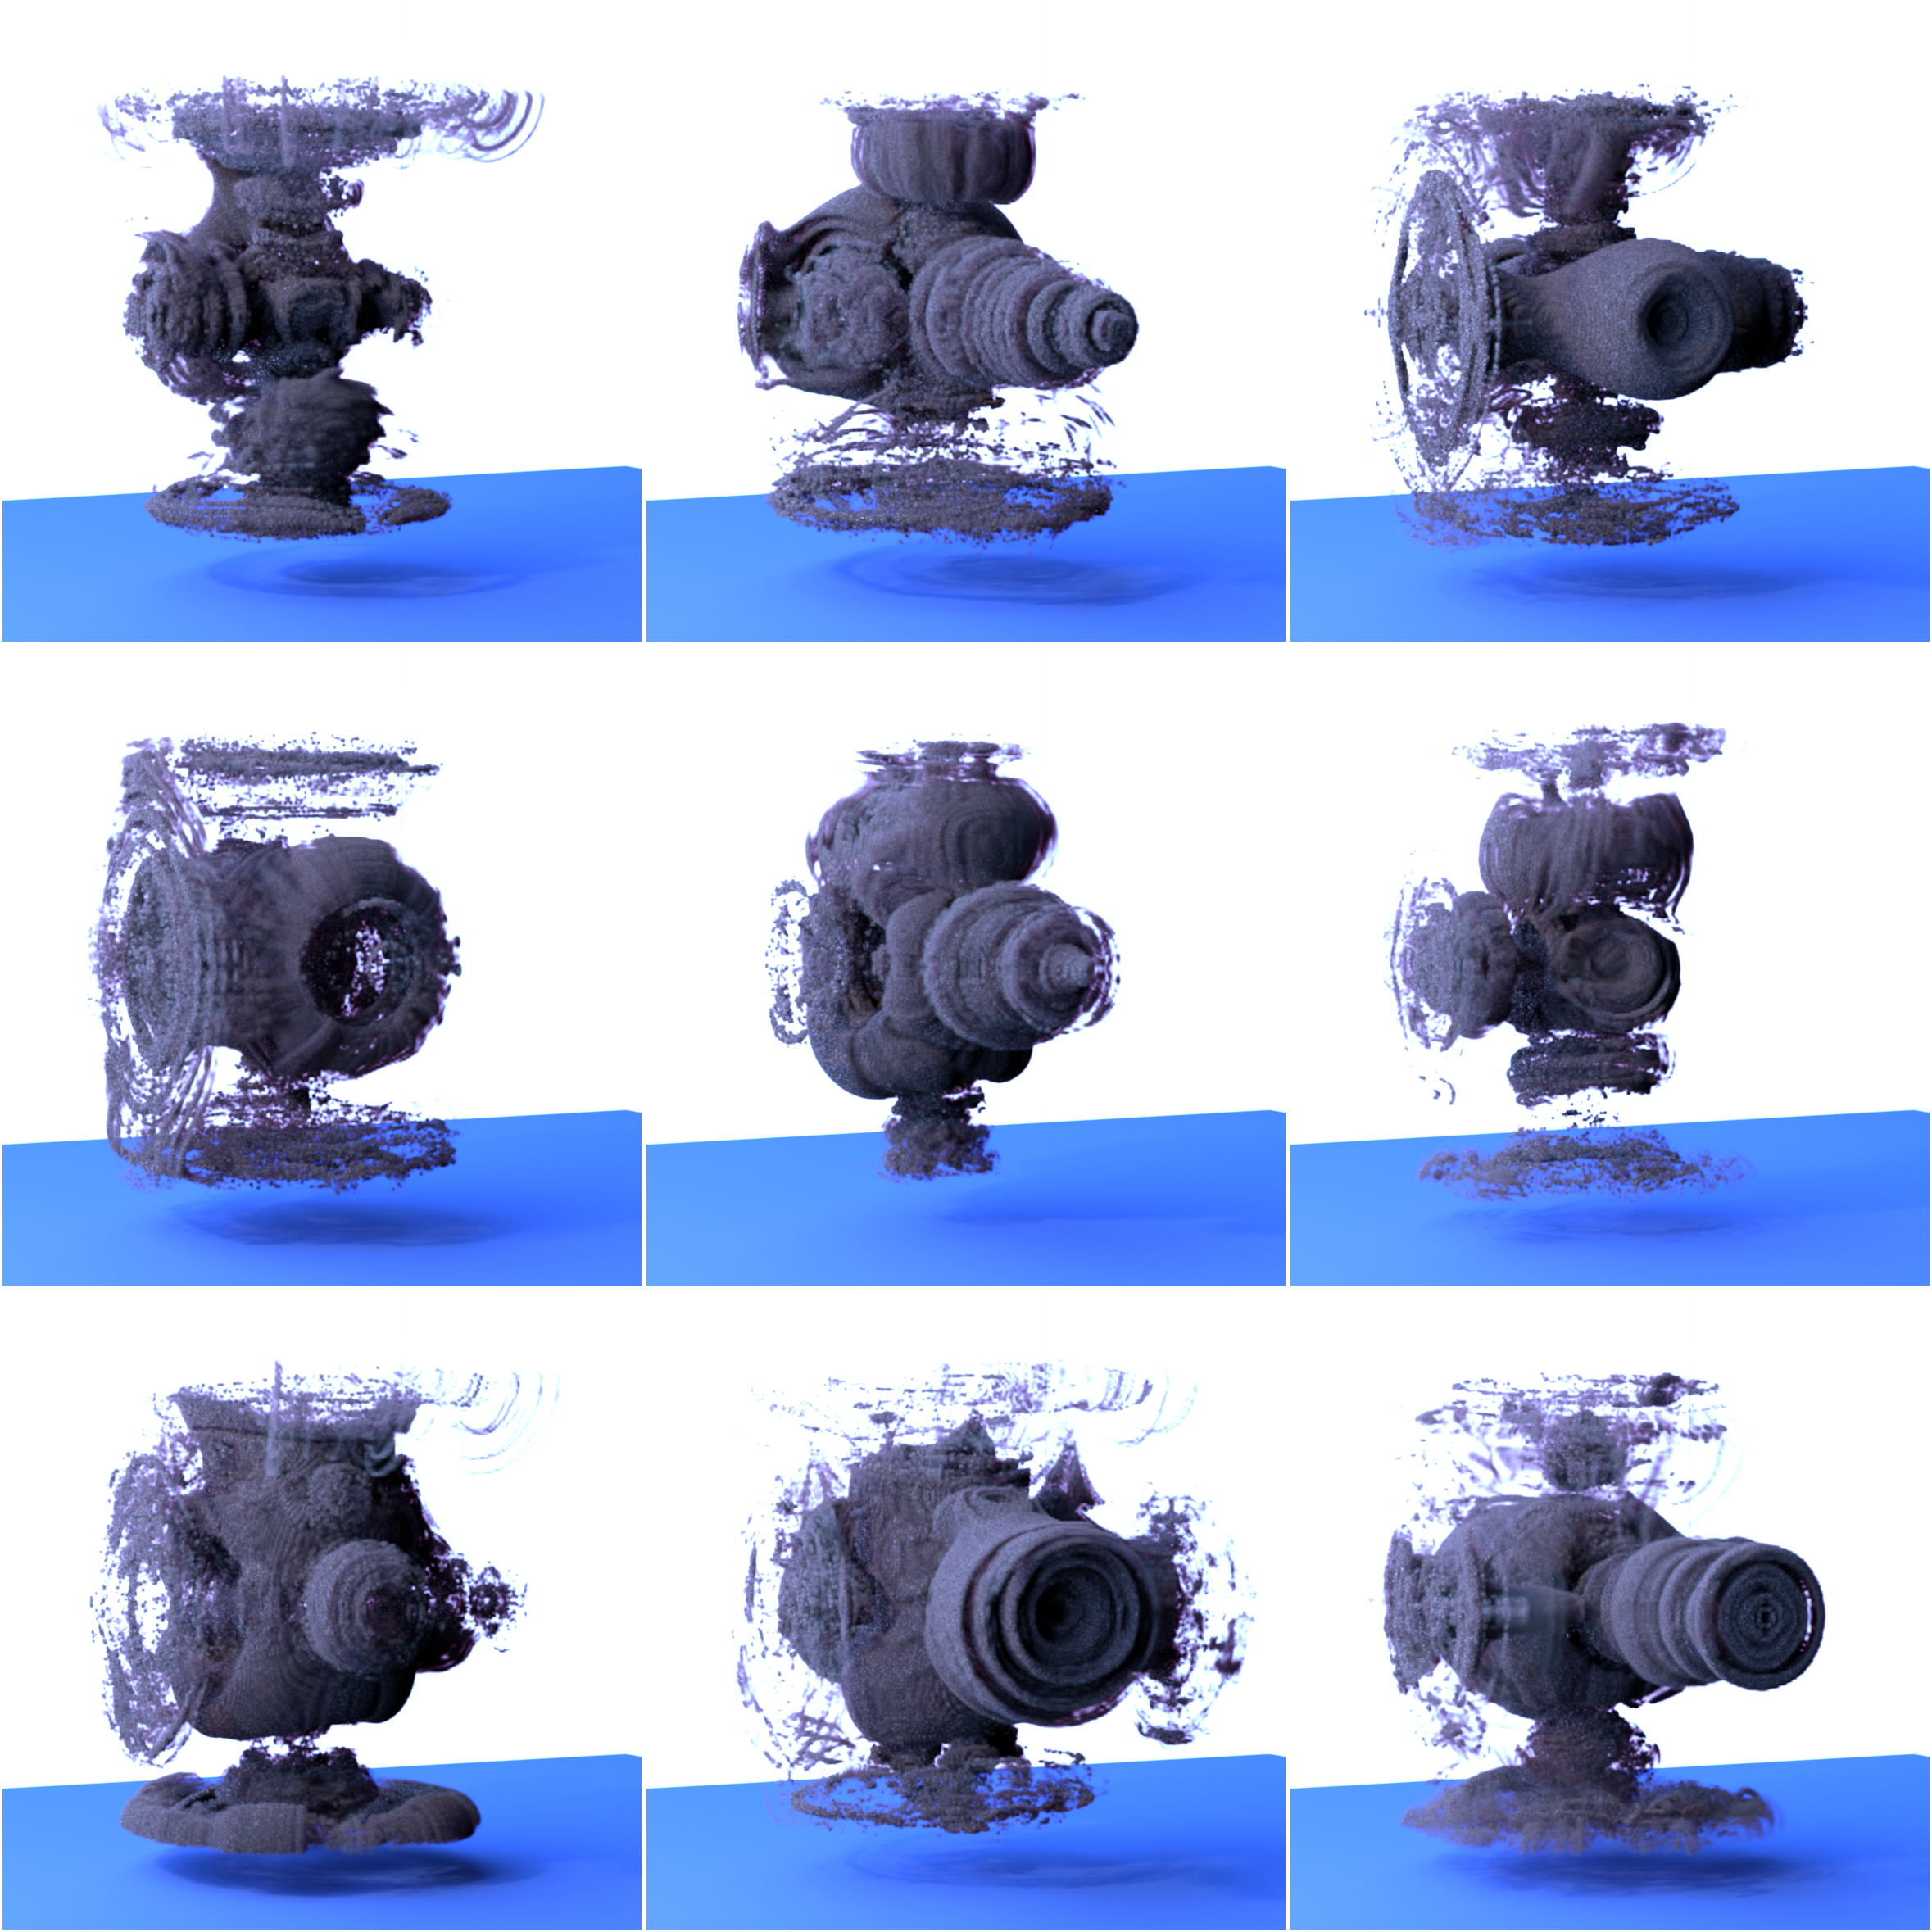
\includegraphics[width=\textwidth]{chap5/figures/modes/montage_recolored.png}
	\caption{\em In reading order: An assortment of nine of the $150$ empirical eigenvectors, from lowest singular value to highest,  discovered by taking the combined SVD of six separate Navier-Stokes simulations.}
	\label{fig:eigs}
\end{figure*}

%%%%%%%%%%%%%%%%%%%%%%%%%%%%%%%%%%%%%%%%%%%
Other excitation strategies are also possible, including ones that are more closely guided by the physics that generated the original input data. We can gradually activate each eigenvector in sequence and then push the resulting vector $\qq$ through a subspace simulation that approximates the Navier-Stokes equations \cite{Kim2013}. Less physical approaches are also possible by treating $\qq$ as a set of mixing weights. We can then construct arbitrary paths $\varphi$, sampled at $T$ time steps $\varphi_1, \ldots, \varphi_T$, that determine the corresponding $T$ time steps of a full-coordinate velocity field. In this vein, we show the fluid simulation that results from a random walk over a higher-dimensional sphere of constant radius in the supplemental video \cite{sphere}.

%%%%%%%%%%%%%%%%%%%%%%%%%%%%%%%%%%%%%%%%%%%
\section*{Sonification}

\begin{figure*}
	\begin{subfigure}[h]{0.5\textwidth}
		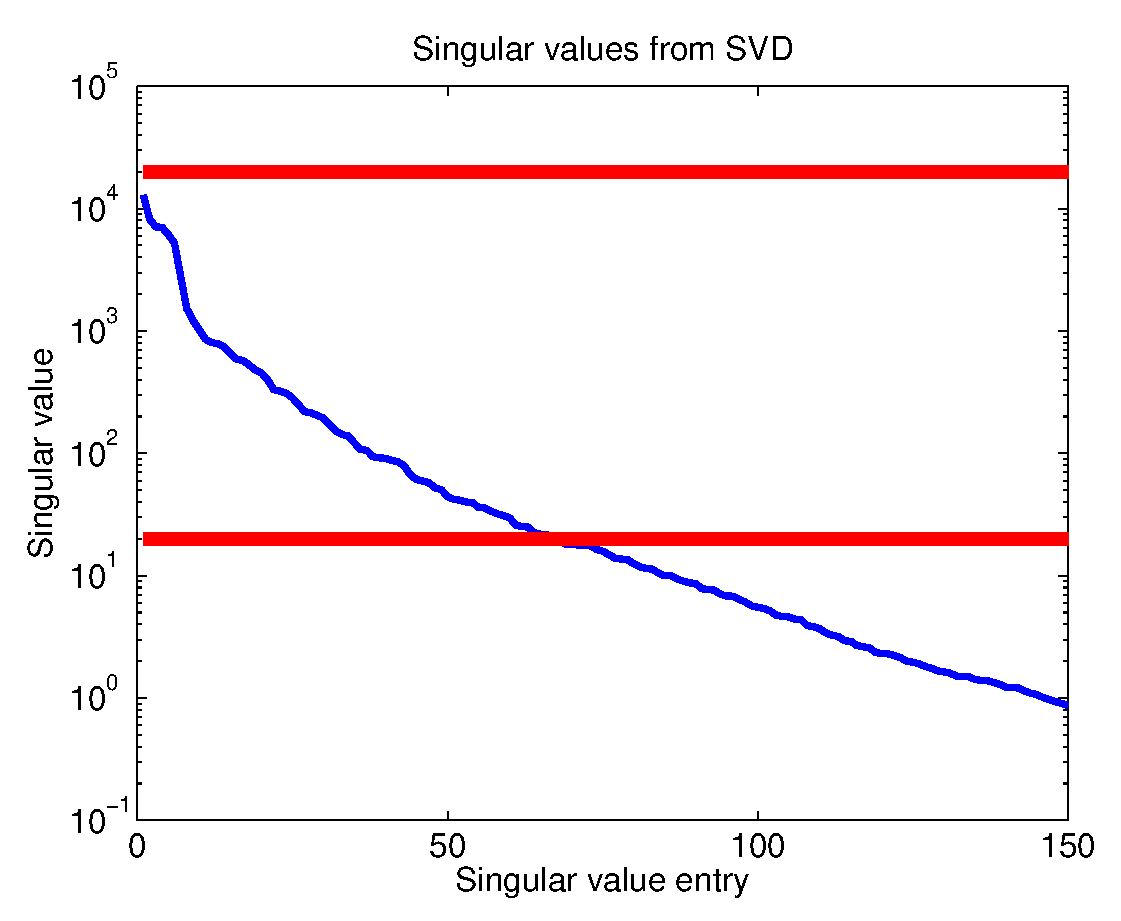
\includegraphics[width=\textwidth]{chap5/figures/singulars.eps}
		\caption{Singular values: $T$ = 150} 
		\label{fig:singulars}
	\end{subfigure}
	%
	\begin{subfigure}[h]{0.5\textwidth}
		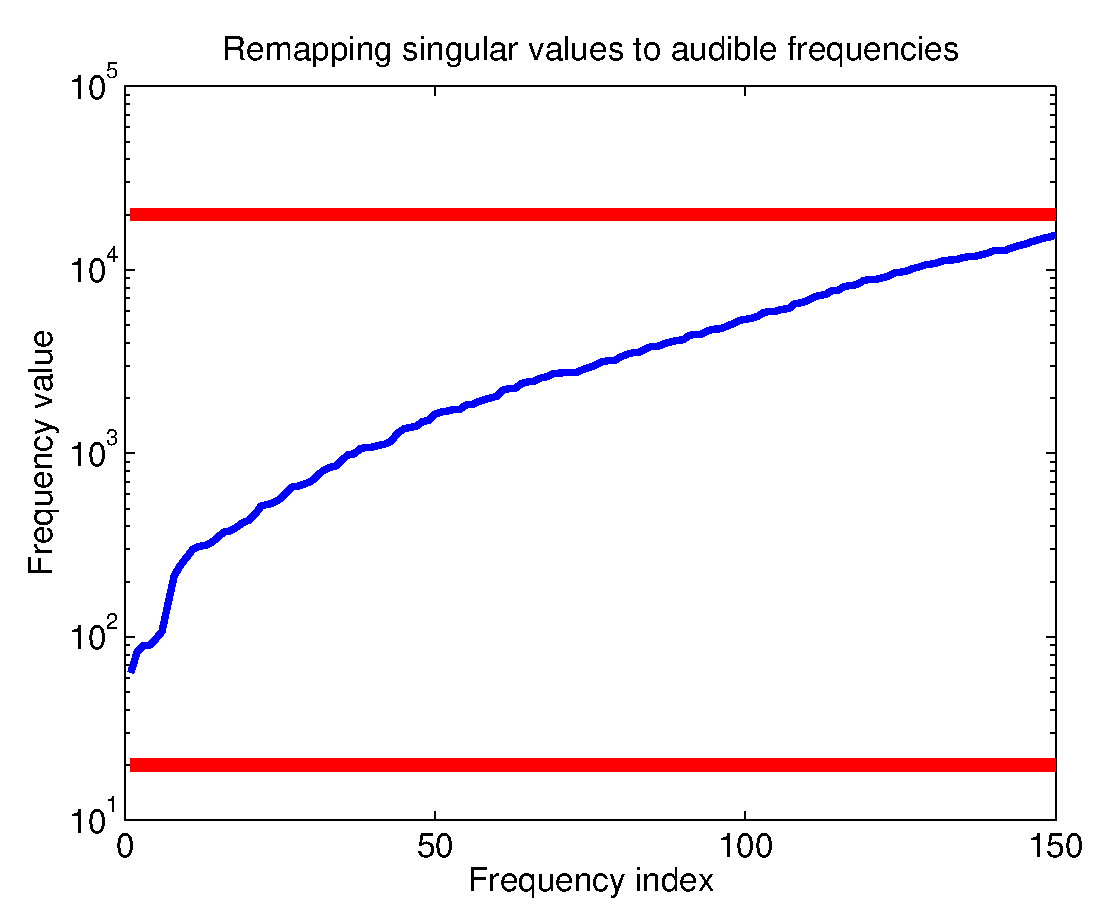
\includegraphics[width=\textwidth]{chap5/figures/remap_freqs.eps}
		\caption{Remapped frequencies: $f$ = 64 Hz, $s$ = 1.75}
		\label{fig:freqs}
	\end{subfigure}
	\caption{\em Singular values and their remapped frequencies. Note the logarithmic scale on both y-axes. The horizontal red lines on both plots indicate the bounds of the human audible frequency range.}
\end{figure*}

We will now devise a strategy for converting the motion of a fluid into a sound. As mentioned previously, one of the main advantages of the empirical eigenvectors approach is that it already yields a quasi-frequency spectrum. However, some additional choices need to be made before these vectors can be made audible. This sequence of subjective but judicious choices is known as sonification. More precisely, according to Hermann \cite{hermann2008}, sonification is the ``data-dependent, systematic generation of sound.''

We begin by interpreting the $T$ singular values $\sigma_1, \ldots, \sigma_T$ from the singular value decomposition as characteristic frequencies. There are two immediate concerns about this raw data. First, we can see in Figure \ref{fig:singulars} that the values range over approximately $4$ orders of magnitude, which is approximately $13$ octaves, and decrease to numbers less than $1$. However, the human audible frequency range begins at $20$ Hz and spans approximately $10$ octaves, up to $20000$ Hz \cite{rosen2011signals}. Thus, we must somehow normalize the data to this audible range. Secondly, the singular value spectrum begins with a maximum value and then decreases, whereas an audio spectrum starts at fundamental frequency and then increases. Hence, we invert the singular values. One way to construct a practical mapping is to specify a fundamental frequency $f$ and an octave scaling $s$. Writing our audible frequencies as $f_1, \ldots, f_T$, we can define our mapping from singular values to audible frequencies as follows:

\begin{equation} 
\begin{aligned}
f_i &= f \cdot \left(\frac{\sigma_{i}^{-1}}{\sigma_{\textnormal{max}}^{-1}}\right)^{\frac{1}{s}} \\
&= f \cdot \left(\frac{\sigma_{\textnormal{max}}}{\sigma_i}\right)^{\frac{1}{s}}, \ i = 1, \ldots, T.
\end{aligned}
\end{equation}

The effect of this remapping can be seen in Figure \ref{fig:freqs}, where we have used a fundamental frequency of $f = 64$ Hz and an octave scaling of $s = 1.75$. The spectrum now begins at the fundamental, $f = 64$ Hz, and ranges up to a maximum of approximately $15000$ Hz, which is an acoustically acceptable spread.

With an audible spectrum established, we now choose amplitudes for each individual frequency. These can be mapped from a corresponding subspace vector $\qq \in \R^T$, as each of its $T$ components, $q_1, \ldots, q_T$ can be thought of as an amplitude for the $T$ corresponding frequencies $f_1, \ldots, f_T$. Care must be taken here to ensure that sum of all the amplitudes does not exceed unity gain, as this would lead to clipping. More concretely, we constrain the $L_1$ norm of $\qq$, $\lvert\qq\rvert_1 = \sum_{i=1}^{T}\lvert q_i \rvert$, to be at most $1$. A typical subspace vector $\qq$ may also contain negative components. However, these can simply be thought of as encoding a positive amplitude and a reversal of phase. The phase reversal can be discarded, as its perceivable effect is typically undesirable clicking artifacts.

With these considerations in hand, we design a mapping from a subspace vector $\qq$ to an amplitude vector $\aaa$ of unit $L_1$ norm as follows:
\begin{equation}
\begin{aligned}
a_i &= \frac{\lvert q_i \rvert}{\lvert\qq\rvert_1}, \ i = 1, \ldots, T.
\end{aligned}
\end{equation}
Given a sequence $(\qq_t)$ of vectors that describe a sampled trajectory $\qq_1, \ldots, \qq_T$ through the subspace $\R^T$, we can normalize each $\aaa_t$ vector individually. Alternatively, we can determine which $\qq_t$ has the maximum $L_1$ norm, which we denote ${\qq}_\textnormal{max}$, and normalize based on $\lvert\qq_{\textnormal{max}}\rvert_1$. The effect of the former is a relatively uniform volume level, while the latter yields a more variable volume envelope. Each approach has its own musical merit depending on the compositional situation.

%%%%%%%%%%%%%%%%%%%%%%%%%%%%%%%%%%%%%%%%%%%
\section*{Synthesis}

With our mappings carried out, we can now produce an audible sound. To illustrate the basic mapping between the visual forms of the eigenvectors and their corresponding remapped frequencies, we move sequentially through the eigenvectors and their corresponding frequencies in the first supplemental video \cite{sequential}. This mapping generates a musical scale, and compositional operations can be carried out at the note level. For example, by scrambling the order of the frequencies and adding some rhythmic variety, we can produce a short melody, as demonstrated in the second supplemental video \cite{melody}.

% ADJ: Here is the code to generate the footnote citations of the YouTube URLs instead:
% {\tt sequential}\footnote{\url{https://youtu.be/cB79S4NwCHc}}
% {\tt melody}\footnote{\url{https://youtu.be/N6fzJXbn2ts}} 

The previous example essentially captures freeze frames of each individual mode. However, a smoother, more sophisticated auditory mapping is needed if we want to capture the flow of the smoke through mixtures of the modes. As a point of departure, we use subtractive synthesis, which passes a spectrally rich input signal through various filters in order to alter its timbre. In our case, we construct a filter bank that attenuates the input signal everywhere except at the resonant frequencies that correspond to the active modes. A particular amplitude vector $\aaa$ with component $a_i$ then tells us the strength with which each corresponding frequency $f_i$ will resonate. The nature of the input sound also strongly influences the resulting timbre: noise creates a more atmospheric effect, while impulses can create driving rhythmic textures. To match the fluid feel of the smoke propagation, we use broadband noise for the primary sound examples in this paper.

%%%%%%%%%%%%%%%%%%%%%%%%%%%%%%%%%%%%%%%%%%%
\section*{Time Evolution}
Static sound, while interesting as a new timbre for a few seconds, eventually grows stale. Thus, we would like to capture the time evolution of the subspace trajectory as a dynamic sonic event. This can be achieved by cycling through the the sequence of amplitude vectors $\aaa_1, \ldots, \aaa_T$ corresponding to the subspace trajectory $\qq_1, \ldots, \qq_T$. Using subtractive synthesis, as described above, we can generate a corresponding sound signal that changes subtly at each time step $t$. As previously discussed, different trajectories through the subspace generate different sequences of amplitude vectors. Musically, the unfolding of these trajectories over time occurs on a micro-scale, but the overall effect is perceived smoothly, much as the individual frames of a video fuse together into a continuous motion.

Experimentally, we have explored several different categories of subspace trajectories. In the third supplemental video \cite{reduced}, we gradually activate each eigenvector in sequence and push the resulting subspace vector through the reduced-space Navier-Stokes equations. In the final supplemental video {\cite{sphere}, we put aside the equations of fluid flow and walk the subspace vector $\qq$ across the surface of a sphere in $\R^T$. 

% ADJ: Here is the code to generate the footnote citations of the YouTube URLs instead:
% {\tt reduced}\footnote{\url{https://youtu.be/_DXRQZYLcdE}}
% {\tt sphere}\footnote{\url{https://youtu.be/y6zraBpH5PA}}

\section*{Conclusion}

We have performed a preliminary aesthetic exploration of the visual and sonic patterns that arise from a generalized form of the Chladni plate experiment. Instead of studying the eigenvectors of a rigid vibration, we computed the empirical eigenvectors associated with fluid flow. The resulting forms are visually striking, and the corresponding spectrum can be sonified to produce a promising compositional palette. Suspending the underlying physics and performing an abstract subspace traversal produces intriguing results, which suggest many possible avenues for future artistic work. The interplay between the audio and the visual shapes seems to form a compositional palette that is worthy of further exploration.

\chapter[Compositional exploration of fluid subspaces]{Compositional explorations of fluid subspaces}
\label{chap:chap6}

With our sonification system from Chapter \ref{chap:chap5} in hand, we now delve into its implications for composition. The process of musical composition, at its core, focuses on different
organizations of time. Commonly, we organize our thoughts and experiments on different timescales: the sound object level, which governs very short durations such as individual notes, the mesolevel, which is an intermediate scale which governs larger groups such as phrases or themes, and the macrolevel, which governs the overall form and structure of a piece of music. The idea of conceptualizing the
organization of music into three hierarchical time levels is especially emphasized in the works of Heinrich Schenker, whose theory of Schenkerian analysis works to unite the structure of musical pieces on the scales of 
foreground, middleground, and background \cite{cadwallader2007analysis}. Further subdivision of time scales have been noted by Curtis Roads, who articulates a total of nine time scales, ranging from the infinite down to the infinitesimal \cite{roads2004microsound}. While this more broad taxonomy is conceptually useful, in practice, composing a piece whose duration is only several minutes does not typically require working at time scales broader than our stated macro level. Additionally, unless the compositional process includes the use of ``microsound,'' or sounds that ``extend down to the threshold of auditory perception," we will also not need to work at time scales shorter than the sound object level. Hence, for our purposes, conceptualizing music in terms of three different time scales shall suffice.

\section{Mode Isolation}
The simplest compositional parameter of interest is the activation or deactivation of individual modes. While a physically accurate subspace re-simulation will, in general, at each time step, require a linear combination of each of the $r = 150$ modes, it is also possible to evolve the velocity fields over time according to algorithmic rules rather than physics-based rules. We imagine the $r$ modes as a sort of configuration space, so that the corresponding $r$ weights map to a particular spatial and aural phenomenon. As such, the most elementary experiment is the sequential activation of one mode at a time, creating a corresponding fluid shape of ``vibration'' which is mapped to its related ``frequency'' according to the system explained in Chapter 5. A low-\footnote{Low: \url{https://www.youtube.com/watch?v=CAoQLYr8doE}}  medium-\footnote{Medium: \url{https://www.youtube.com/watch?v=Vwpi6U7AD5A}} and high-frequency mode\footnote{High: \url{https://www.youtube.com/watch?v=o0UtONgtpFo}} are each shown isolated in the referenced videos. 

Because each mode in isolation can be regarded as a musical note, this strategy allows us to carry out musical composition on the note level, producing simple melodies. Without a principled way to choose a rhythm,
however, we are left only to general aesthetic considerations. An example of such a mode-based melody \footnote{Melody: \url{https://www.youtube.com/watch?v=N6fzJXbn2ts}} is demonstrated in the referenced video. (Figure \ref{fig:melody} shows a single 
frame from the video for reference.)

\section{Mode Superposition}
The next experiment to try is the superposition of modes, creating mixtures of the modal vibration shapes in the spatial domain and harmonies in the audio domain. Again, the physics-based time evolution governs a complex coupling of the modal weights that resists simple exploration, so we turn to simple algorithmic rules to better understand the system. We can see the result of mixing a low-, medium-, and high-frequency mode with equal proportions.

\begin{figure}[H]
	\centering
	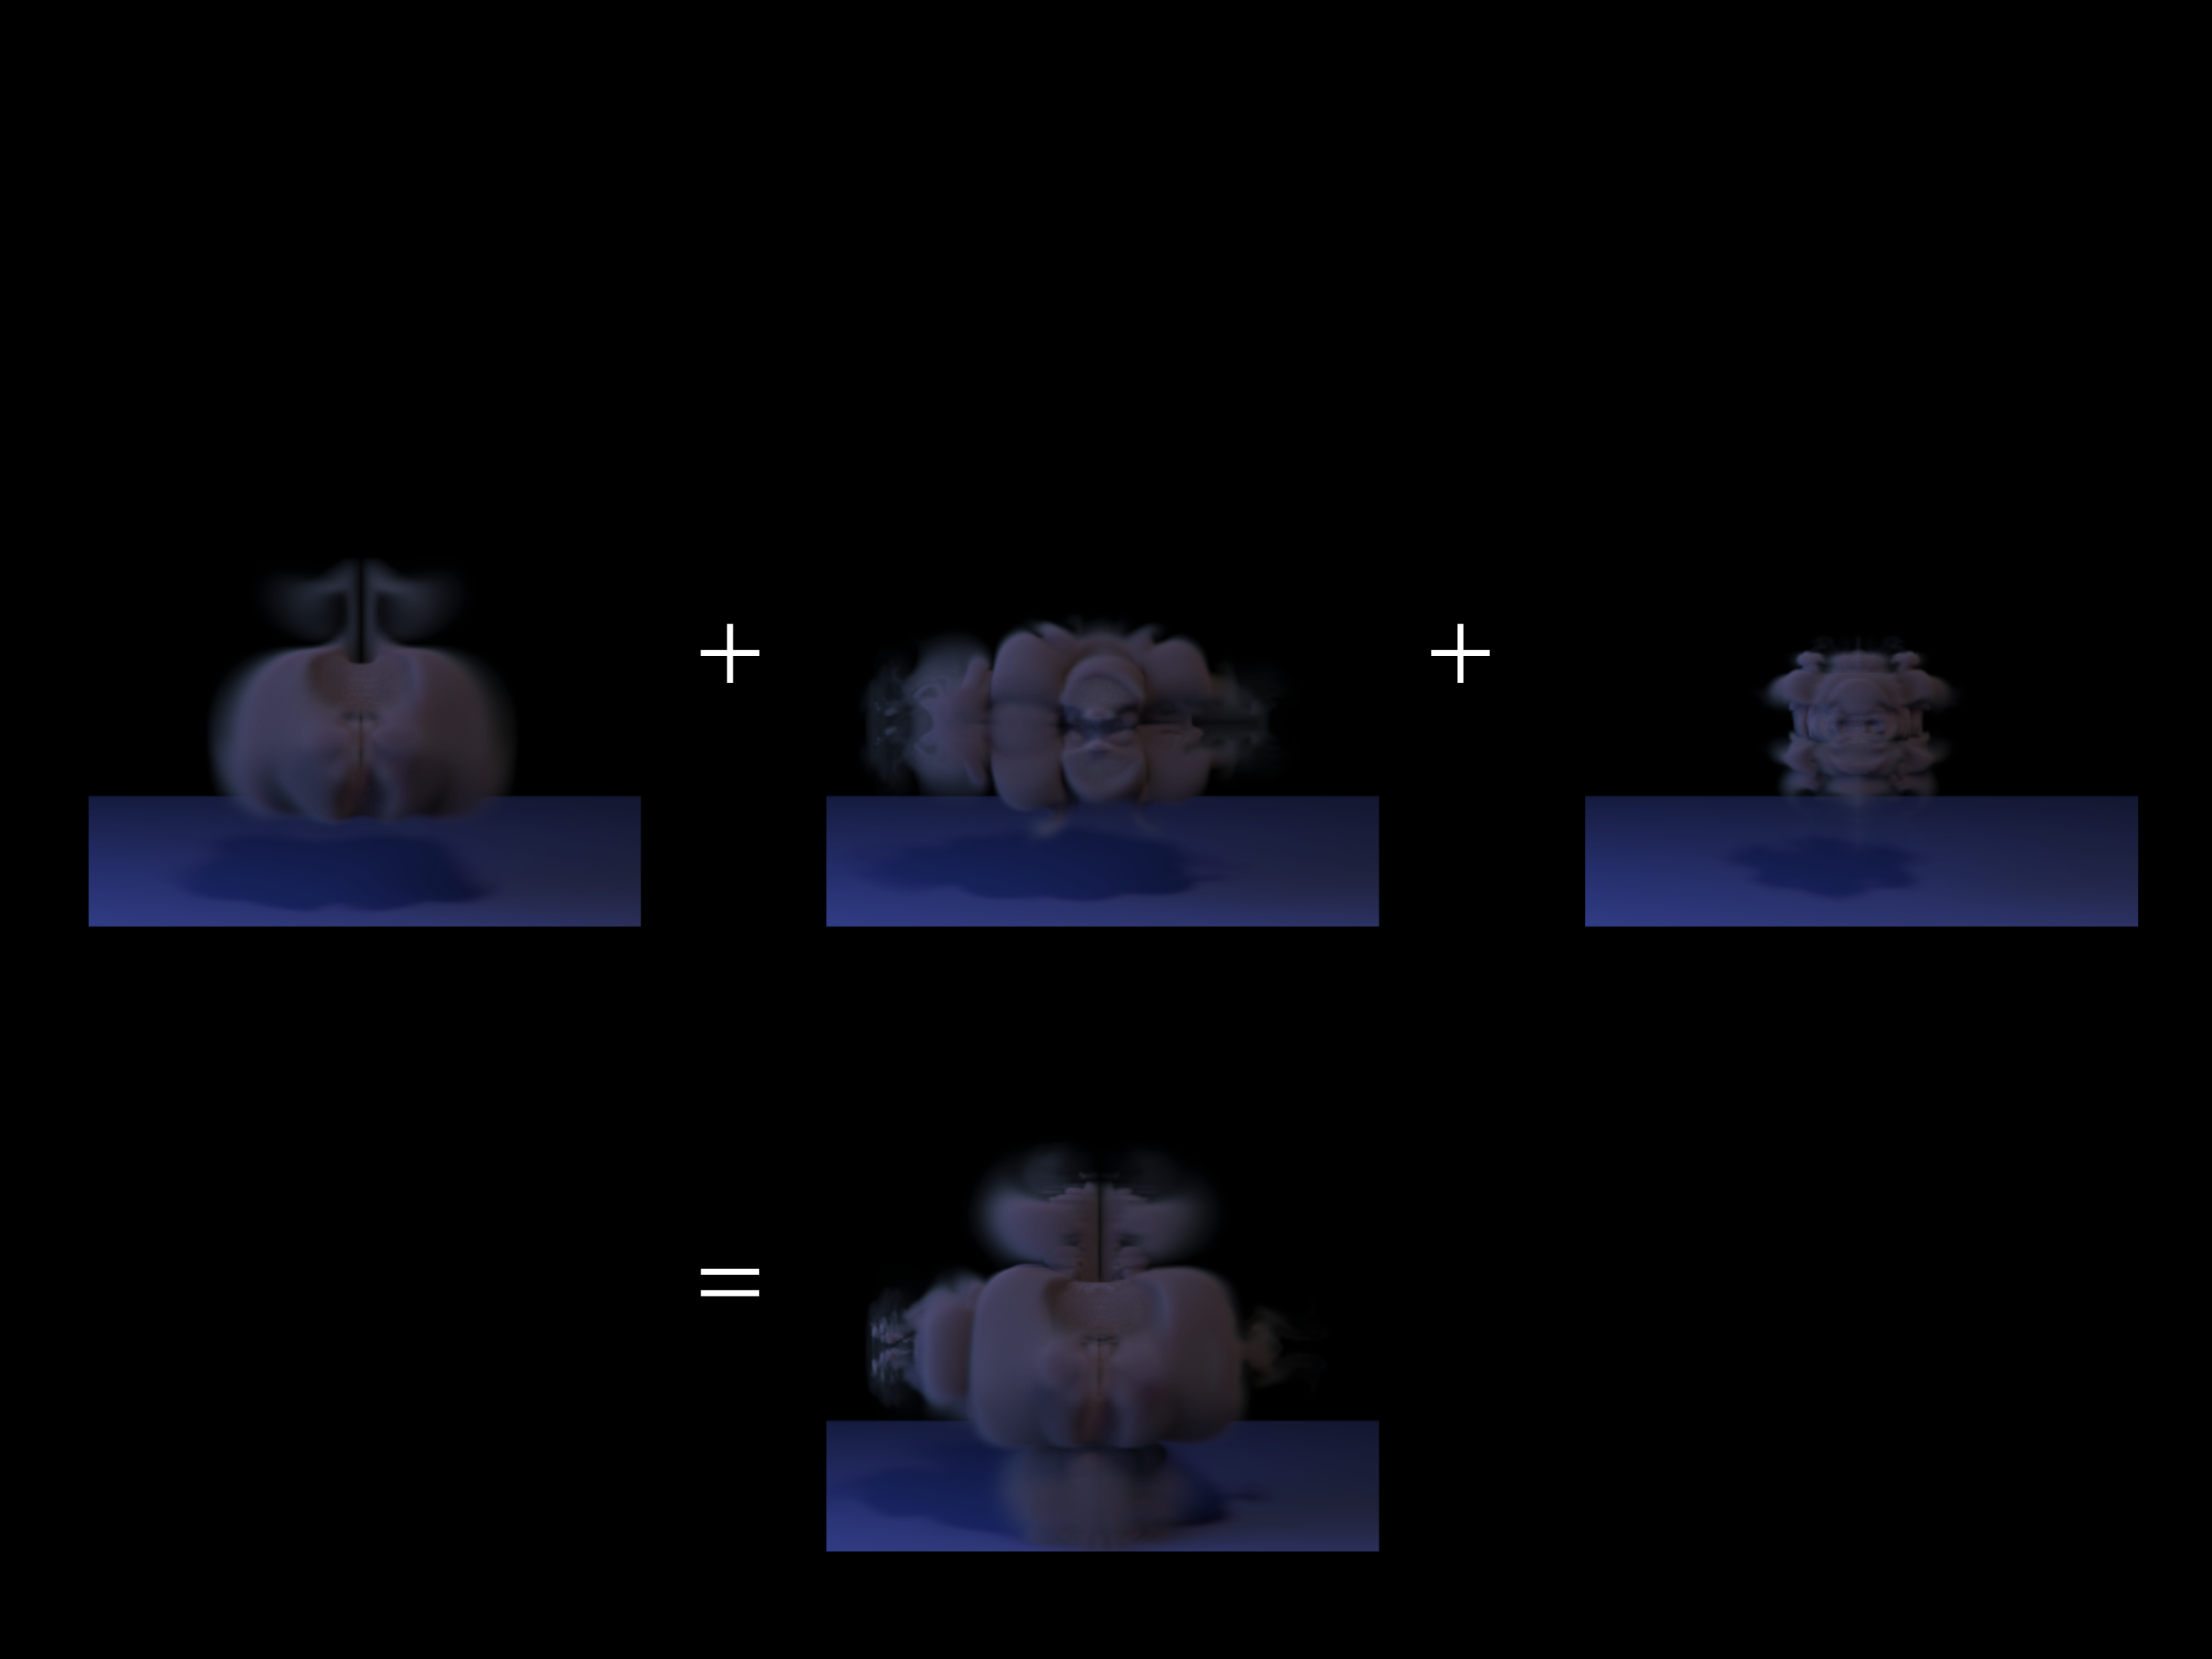
\includegraphics[width=\textwidth]{chap6/figures/superposition.png}
	\caption{\em Three individual modes in superposition produce a mixed modal shape.}
\label{fig:superposition}
\end{figure}

\section{Dynamic Control}
If we define the {\em energy} of a fluid snapshot in time as the $L_2$ norm of the vector of modal weights, then we see that as time unfolds, the energy waxes and wanes according to the strength
of the various modal weights. Accordingly, the sound increases or decreases in overall spectral density and loudness based on the same principle. However, by forgoing the physics-based time-evolution,
we can harness direct spectral control over the visuals and sound, producing simple and pleasing audiovisual gestures such as crescendo, diminuendi, and swells. An accent followed by diminuendo \footnote{Accent: \url{https://www.youtube.com/watch?v=0An95mF3Yk0}}, and a crescendo-diminuendo swell \footnote{Swell: \url{https://www.youtube.com/watch?v=zUkpNKpkwP4}} are each shown in the referenced videos, accompanied by still frames in Figures \ref{fig:dim} and \ref{fig:swell}, respectively.

\begin{figure}[H]
	\centering
	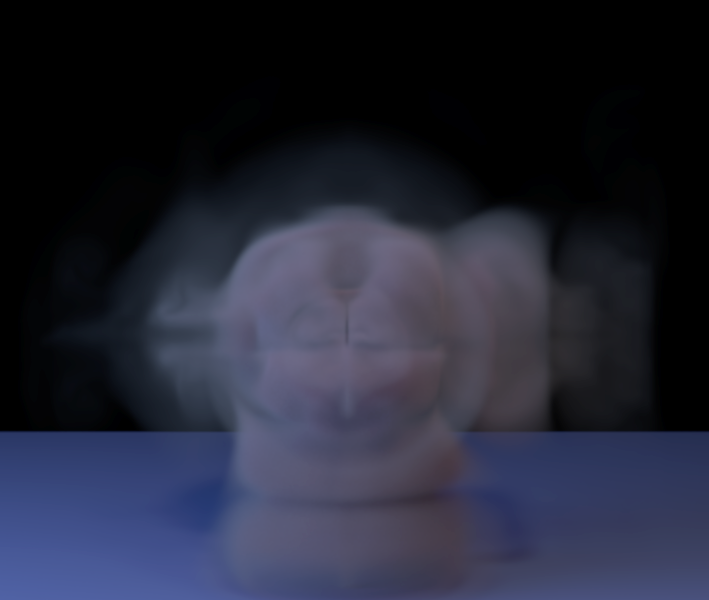
\includegraphics[width=\textwidth]{chap6/figures/dim.png}
	\caption{\em A still frame from the accent followed by diminuendo video.}
\label{fig:dim}
\end{figure}

\begin{figure}[H]
	\centering
	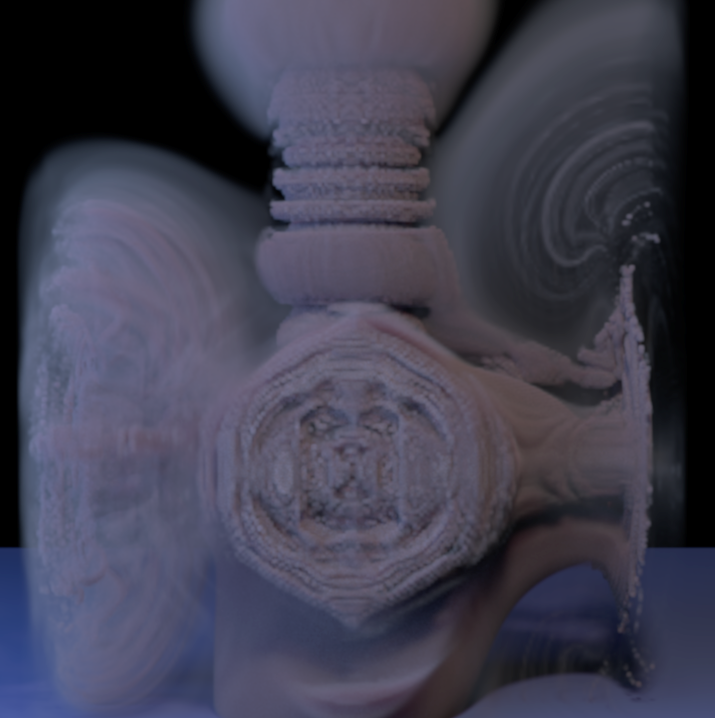
\includegraphics[width=\textwidth]{chap6/figures/swell.png}
	\caption{\em A still frame from the crescendo-diminuendo swell video.}
\label{fig:swell}
\end{figure}

\begin{figure}[H]
	\centering
	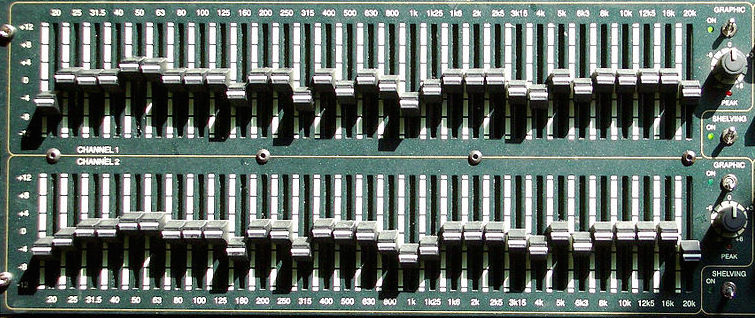
\includegraphics[width=\textwidth]{chap6/figures/faders.jpg}
	\caption{\em Each of the $r = 150$ modes can be controlled individually, analogous to a set of equalization faders. Source: Wikimedia Commons.}
\label{fig:faders}
\end{figure}

\section{Mode Coupling and Envelopes}
The simultaneous activation of all modes produces a spectrally rich sound quality, or timbre\footnote{According to ANSI 1960,
"Timbre is that attribute of auditory sensation in terms of which a listener can judge that two sounds similarly presented and having the same loudness and pitch are dissimilar. [. . .] Timbre depends primarily upon the spectrum of the stimulus."}, not dissimilar from noise. However, more refined filtering leads to a sparser spectrum, yielding a sound quality similar to musical chords. This filtering
can be achieved simply by activating only a small subset of the $r = 150$ modes at once, much as in the mode superposition study. However, such a chord is static over time, creating a dull musical effect for any prolonged 
duration. We can inject extra life into these chords by modulating their {\em envelopes}---i.e., creating time-varying amplitude envelopes around each mode. This strategy is akin to slowly adjusting the different fader knobs 
from high to low at different speeds. A simple mathematical collection of envelopes are sinusoids at different frequencies,\footnote{Oscillation: \url{https://www.youtube.com/watch?v=6nEVXFkWSZ4}} as the referenced video example illustrates. 
(Figure \ref{fig:osc} shows a single frame from this video for additional reference.) Visually, the shapes morph in and out of a slow cycle of superpositions, while the sound fades in and out of subtle frequencies of an overall chord.

\begin{figure}[H]
	\centering
	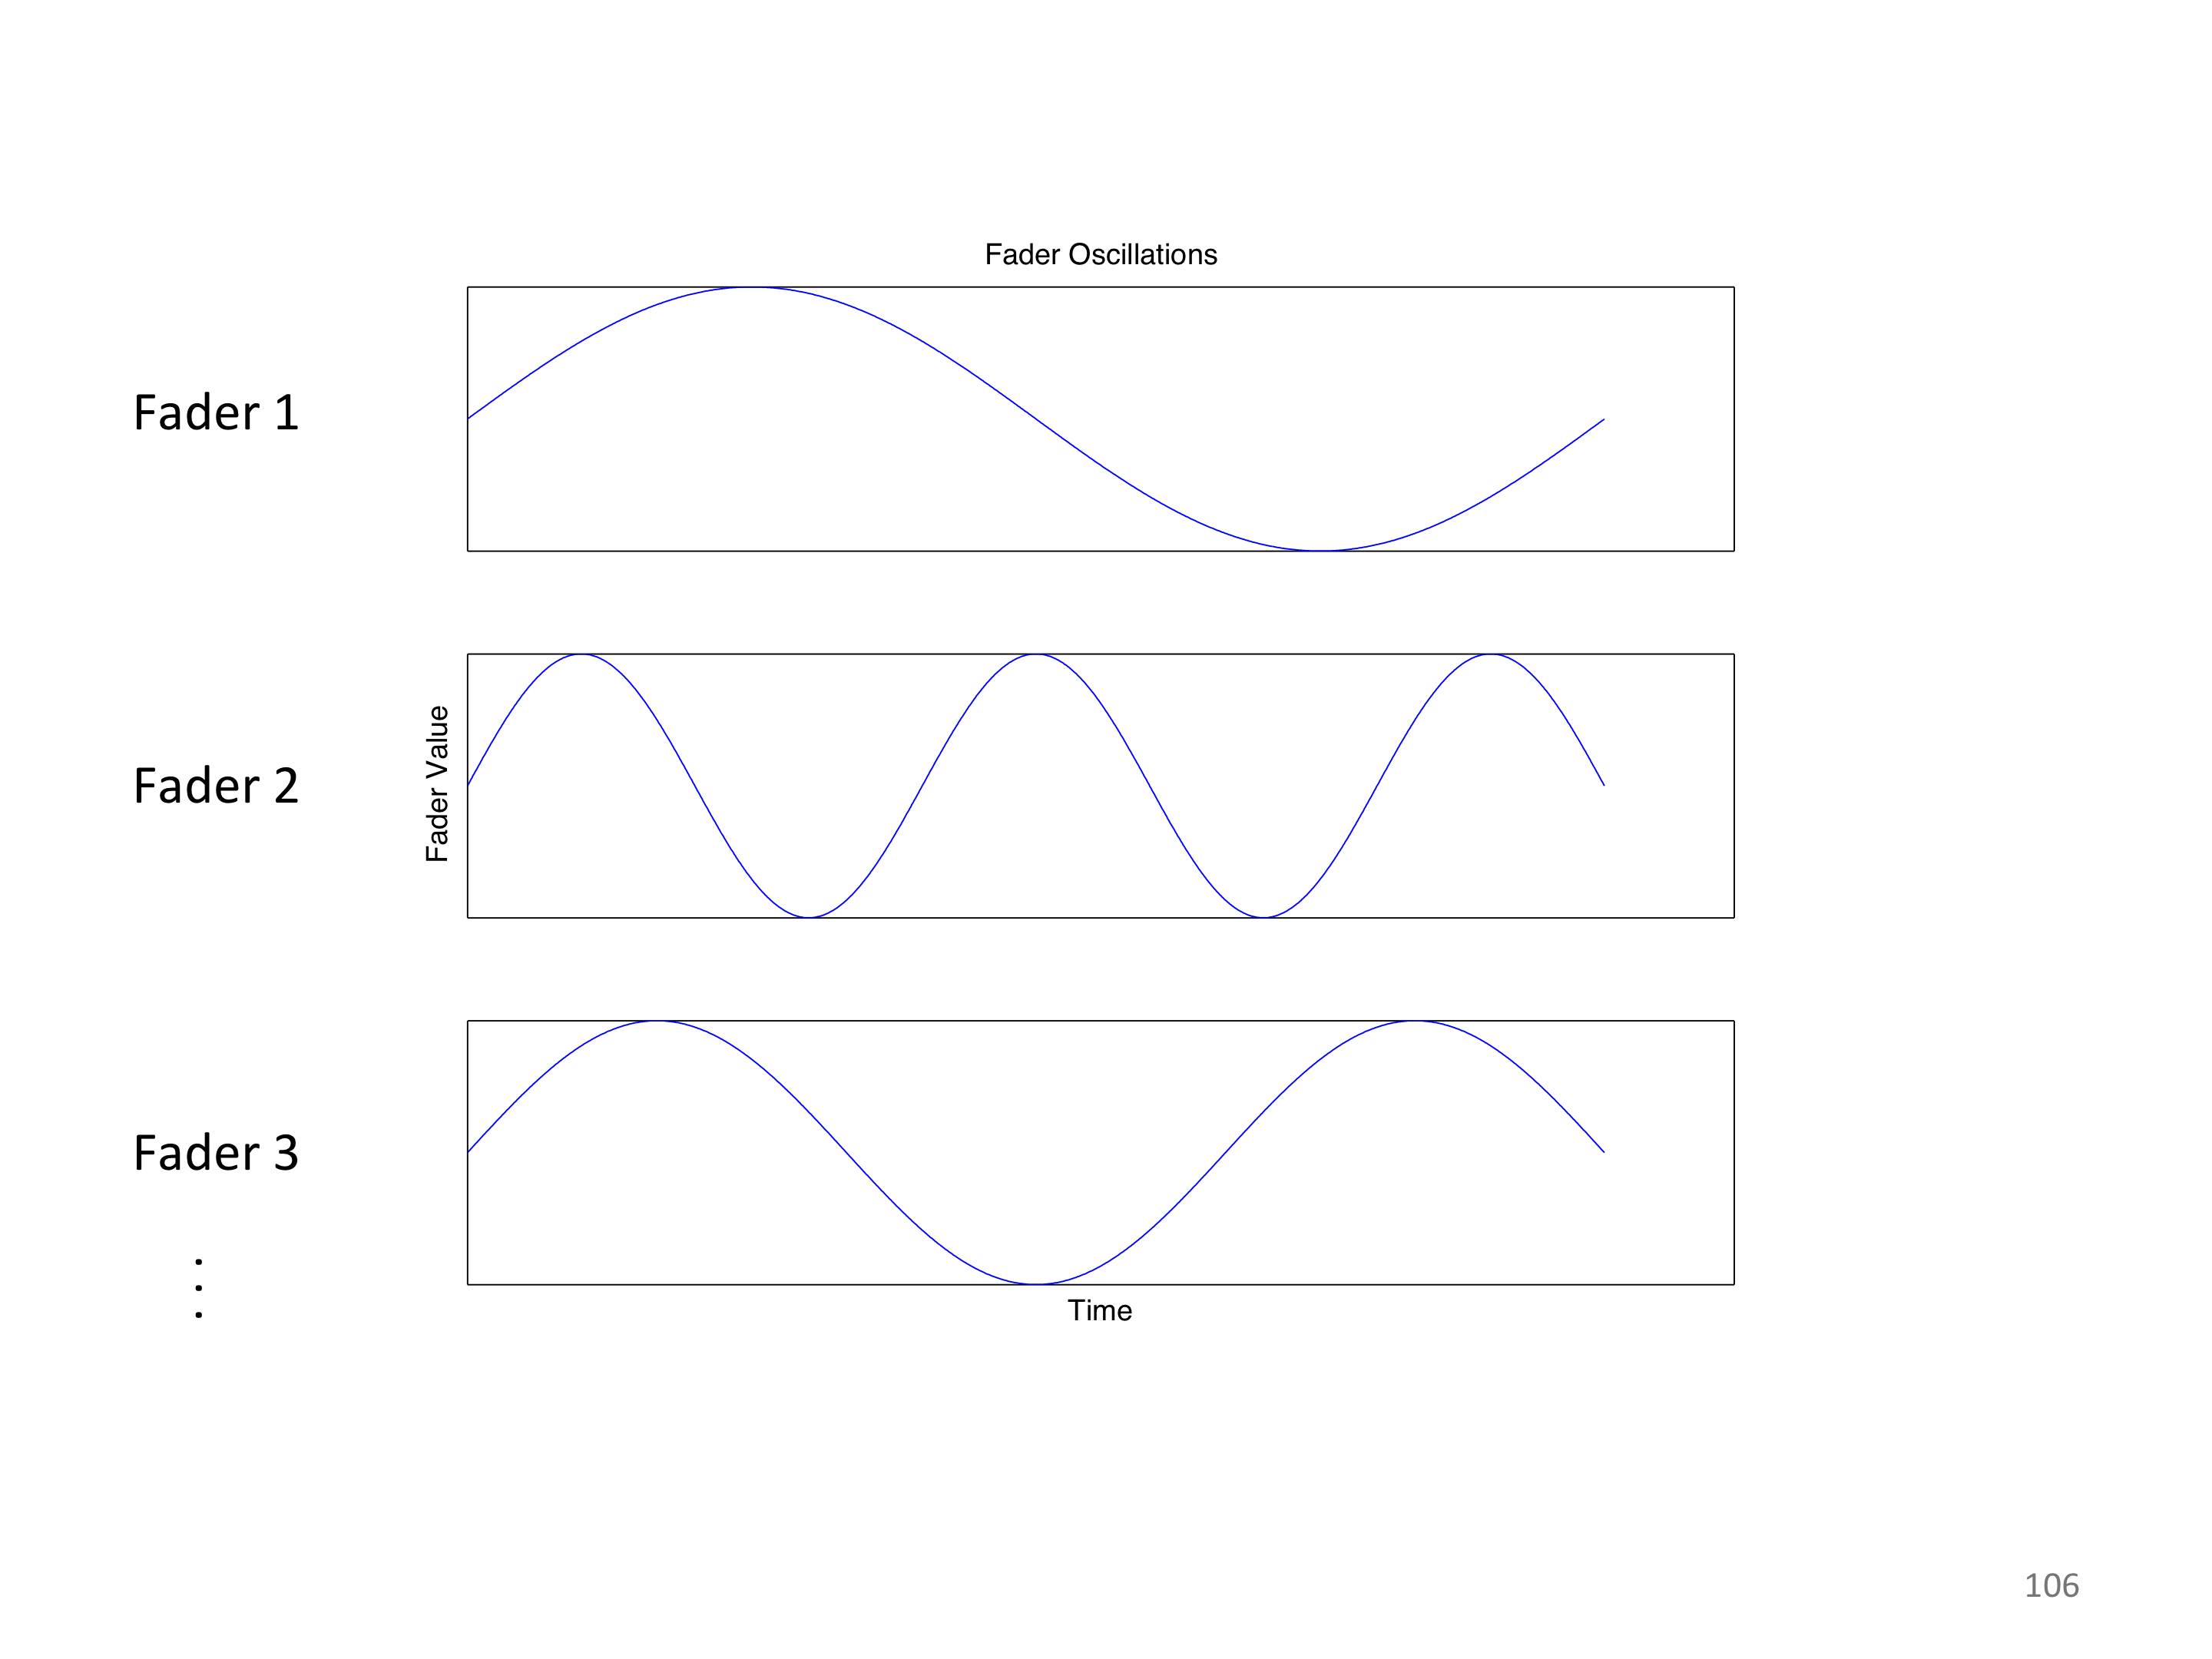
\includegraphics[width=\textwidth]{chap6/figures/fader_envelopes.png}
	\caption{\em Each modes's fader knob can be modulated smoothly over time, creating spectrally-varying envelopes.}
\label{fig:fader_envs}
\end{figure}

\begin{figure}[H]
	\centering
	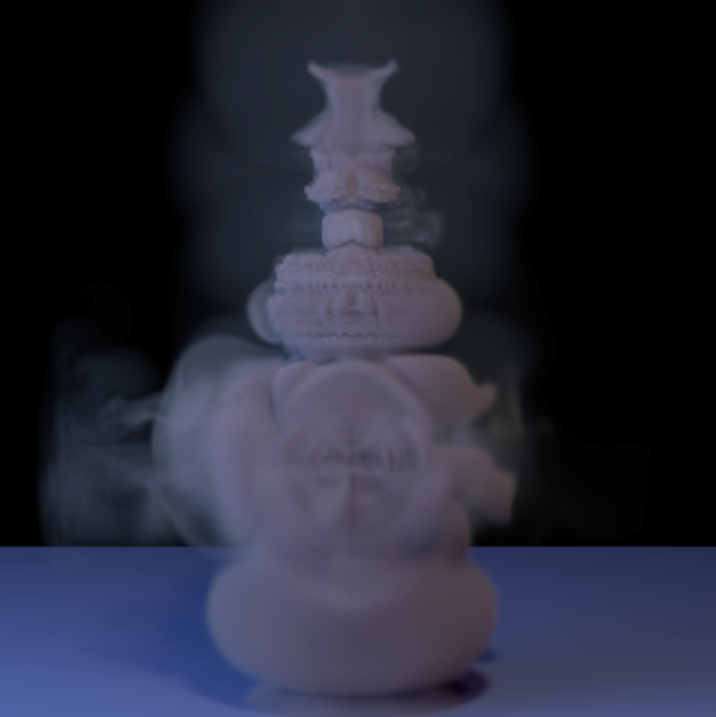
\includegraphics[width=\textwidth]{chap6/figures/osc.png}
	\caption{\em A single frame from the oscillation video generated by using time-varying sinusoidal envelopes of a chord.}
\label{fig:osc}	
\end{figure}

We can also {\em couple} different modes together, or transfer from one collection of modes smoothly into another, in analogy to a musical chord progression. (Coupling the modes is also inspired by the
complex nonlinear coupling induced by the real physical phenomenon of advection that we are simulating.) As time evolves, both the amplitude envelopes and the
spectral content itself shifts, producing a complex visual and audio effect\footnote{Crossfade: \url{https://www.youtube.com/watch?v=RCIuZaWqvds}} as seen in the referenced video example. (Figure \ref{fig:cross} shows 
a single frame from this video for additional reference.)

\begin{figure}[H]
	\centering
	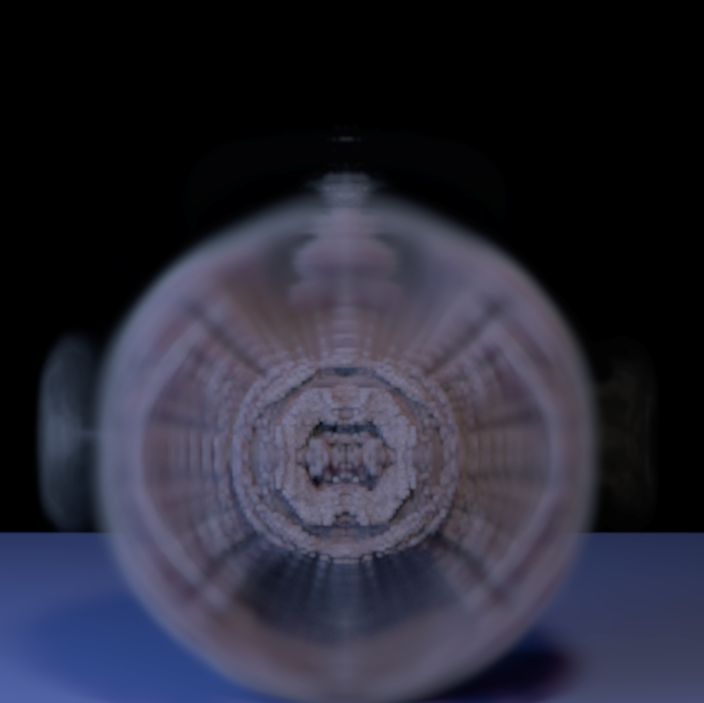
\includegraphics[width=\textwidth]{chap6/figures/cross.png}
	\caption{\em A single frame from the crossfade video generated by modulating both the amplitude envelopes and spectral content.}
\label{fig:cross}
\end{figure}

\section{Sonification Choices}
Now that we have seen the potential of our sonification system in action, we return to the justification of the many aesthetic choices made in designing it. We have an overwhelming freedom of choice here. In particular,  there is the choice of the physical training set, the choice of mapping between the dynamical system and the audio, and the choice of aesthetic stance. In the following sections, we will consider these issues in detail.

\subsection{Training Data}
Because our system relies on the empirical eigenvectors of a set of training data, the first choice we make in designing our system is the selection of the training data. An insufficiently rich training set will generate a series of results that are limited in dynamic variety due to the nature of the subspace algorithm. Early experiments in this direction were unsuccessful, as the collection of eigenvectors formed results that almost exactly mimicked the full-space simulation from which they were generated. Thus, the idea of using a sequence of full-space simulations was a natural attempt to mitigate this issue. However, since the eigenvectors are agnostic to time, it is useful to construct a sequence of simulations that are very distinct from one another. Hence, our strategy of modifying the direction of buoyancy was appealing. This technique results in six different outward-facing plumes, each of which having its own unique dynamics. The inherent symmetry to this strategy is also appealing from an aesthetic standpoint, as by privileging no one direction over another, the eigenvectors acquire a more abstract quality, detaching them from the more scientifically-grounded full-space simulation. As a result, the empirical eigenvectors take on a series of aesthetically pleasing turbulent forms, ideally suited for generating novel audiovisual compositions.

\subsection{Sound Synthesis}
As discussed in Chapter \ref{chap:chap2}, the details in implementing a system of sonification allow for a wide freedom of choice. Hence, it is important to justify our choices by perceptual or aesthetic concerns. We identify and discuss several of our choices in this section.

Perhaps the choice that influences most the character of our auditory results is our choice for sound synthesis. No matter what mapping we choose from physics to sound, the engine which produces actual audible sound influences the output tremendously. Thus, our choice of using subtractive synthesis of spectrally rich noise deserves further investigation. Indeed, our initial concept utilized a simpler system of additive synthesis. However, we found the subtractive synthesis more suitable to our aesthetic needs for several reasons.

Firstly, our system produces not just sound, but sound and visuals. Aesthetically speaking, we desired a reasonable congruence between the character of both the audio and the visual domain. In particular, although the dynamics of the visuals varied substantially, the overall look and feel did not---the simulations were all fluid dynamics of smoke billowing about smoothly. Thus, we immediately discarded many audio results that were choppy and robotic, as the resulting incongruence was displeasing aesthetically. We also discarded a quantized scale such as 12-tone equal temperament, feeling that its rigidity would belie the abstract amorphous quality of our visuals. Therefore, what remained to explore were ambient, textural sounds. Both additive and subtractive synthesis seemed promising, as we had in hand a collection of frequencies from our mapping scheme. While additive synthesis is simple and effective, its results tend to be too sterile for our taste. The individual sinusoids are too digitally clean, and their superpositions result in a computer-like purity that also belies the messy, turbulent swirls of our visuals. Hence, we turned our attention to subtractive synthesis. As discussed in Chapter \ref{chap:chap2}, in some sense, subtractive synthesis is a logical choice, as the entire concept of modes of vibration that our sonification system depends on is built on the foundation of subtractive synthesis. Moreover, by varying the input signal to the filter, a variety of different timbres can be generated. In contrast, additive synthesis produces one single result, which must then be additionally filtered and adjusted to produce pleasing outputs. We settled on using gray noise, which emphasizes the lower frequencies in its spectral output, to bring out the principal singular values more prominently \cite{wilson2011supercollider}. It must be mentioned that the choice itself to map the principal singular values to lower frequencies---that is, a choice of polarization, as discussed in Chapter \ref{chap:chap2}, is itself somewhat arbitrary. However, this choice rests on perceptual considerations, not aesthetic ones. The prominent sonic tones in any timbre are the fundamental frequencies, which are the lowest frequencies; hence, inverting the singular values to match this prominence is a natural and justifiable step to take.

\subsection{Real-Time and Non-Real-Time Strategies}
One of the potential drawbacks of our audiovisual system is its heavy computation cost. As a result, the capacity for real-time interaction is infeasible as of time of writing in 2017. However, the dynamics of non-real-time composition allow for a different 
type of compositional process than a real-time system would afford. In this section, we discuss a few pros and cons of each of these types of systems, illustrating our non-real-time approach while suggesting a roadmap to eventual real-time strategies.

By its nature, a non-real time system lends itself better toward careful structural planning. Pieces must be planned and executed ahead of time rather than as a flash of inspiration. Hence, formal structures flourish, and strategies for unifying a
piece on different time scales become very attractive. The possibility of unifying the material of a piece in the micro-, meso-, and macro-time scales is aesthetically powerful, and only possible through non-real-time composition. As a result, pieces that
are designed with a non-real-time process tend to be structurally sound and aesthetically coherent.

However, the high degree of structure of non-real-time strategies can also be a weakness. The capacity for free improvisation and interaction through real-time often produces unexpected and daring results. Feedback through interaction with the system and having the system ``interact back'' can be extremely rewarding, leading to new insights and promising directions that would otherwise be impossible to discover. Additionally, the ability of the audience to participate in a piece through interaction changes the very nature of the piece. A viewer/listener no longer must let the experience wash over them; instead, they participate actively in the creation of the piece themselves, defining their own new experience which is distinct from all other viewers' experiences.

Ultimately, the non-real-time strategies employed in this dissertation proved effective, as the audiovisual studies were only possible from designing a careful strategy of moving through the subspace according to either mathematical or physical rules. However, the capacity for a real-time interaction to generate unexpected new insights and results from this system remains to be seen, and is a promising direction for future work. Interaction could happen on many levels. For example, the interaction could adjust physical parameters, by introducing new obstacles to the simulation or adjusting the buoyancy or vorticity of the flow. Alternatively, the interaction could be more gestural, allowing the user to control the energy of the system, creating dynamical swells and frequency sweeps as demonstrated by the earlier studies in this section. 

\subsection{Aesthetics}
In our creation of these studies, we imposed our own aesthetic values to some degree on the sonification system to produce musical results. While some sonifications remain purely scientific, created only for the purpose of identifying patterns in data, our own system was always born out of a desire to create musical outputs. The tension between adhering to fixed scientific principles and generating aesthetically interesting musical output is  a constant challenge in composing generative music of this kind. Our aesthetic take, as discussed in Chapter \ref{chap:chap2}, is a middleground between these two extremes. While a system itself can be aesthetically pleasing in the mathematical sense, this is no guarantee of the quality of its musical output. Conversely, a total abandonment of the systematic approach simply for the reasons of adjusting the musical output largely negates the point of composing using such a system in the first place. To that end, our musical adjustments remained of a minor quality, not abandoning the logic of the system, but merely adjusting it in certain cases to compensate for the quality of the musical output. For example, when we take our amplitude mapping from the numerical data of the simulation, all sign information is neglected, as a positive and negative amplitude in sound merely represents an unpleasant phase distortion. While this approach arguably throws away a dimension of the physical data, it does not fundamentally detach the result from the system, and is thus considered acceptable from our aesthetic point of view.

One of our principal aesthetic goals toward future work is the idea of simulating smoke under more fanciful systems of time-evolution than standard physics. Hence, many of our examples play with the idea of controlling the time evolution in different mathematical procedures rather than sticking with the correct physics. While this again is pushing the boundaries of our original system, we nonetheless retain the same link between the visual and audio results. Thus, we view this form of modulation as
a robust way to explore new compositional forms. Changing the underlying rules which govern the time-to-time behavior of the audiovisual system is not the same as abandoning the system; in fact, it has proved fruitful in generating novel results. These strategies move us more in the direction of simulating fluids ``as they might be'' vs. fluids ``as they actually are.''
\chapter[Conclusions and future work]{Conclusions and future work}
\label{chap:chap7}

In this dissertation, we strove to develop a generative audiovisual compositional language. Toward this end, we presented a sonification system for computational fluid dynamics
based on the method of subspaces. Additionally, we devised a data compression algorithm that alleviates the memory costs of subspace algorithms by an order of magnitude. Through
systematic experimentation and exploration, our sonification system was tested and explored, producing a series of audiovisual etudes. The data compression algorithm was tested 
on a variety of different types of scenes, perturbations, and compression levels, demonstrating its general robustness and effectiveness. Continuing research in the direction of the sonification
system is an important step in the development of new audiovisual grammars in media art, while further work in the area of data compression represents an important step toward
making subspace simulations more computationally practical.

 \section{Summary of Results}
 We have devised a system of sonification of computational fluid dynamics by considering the empirical eigenvectors and eigenvalues of a subspace simulation. Based loosely on the ideas of 
 Chladni plates and the general conception of cymatics, we map the characteristic resonant modal shapes of the fluid velocity field bases to their corresponding audio frequencies,
 producing a sound signal. The choice of a model-based sonification strategy allows us to unfold our visuals and sounds over time within the framework of the system. Hence, the natural
 sequence of fluid velocity fields as governed by the subspace Navier-Stokes equations determines a natural time progression of dynamic visual forms and sonic content. 
 
 Several sound synthesis strategies and transformations had to be considered. We carefully mapped the raw singular values into frequencies,
 choosing an intuitive polarization as well as a ratio-preserving transformation and offset to keep the values within the limits of human hearing. Following the spirit of physical modal vibrations, we 
 selected a subtractive synthesis technique, in which a filterbank of resonant filters at the corresponding modal frequencies were excited in various strengths and decay times. Although many possible
 input signals could be used with the filter bank, we chose to use noise, as it was both spectrally rich and matched the aesthetic feel of fluid flow.

Our audiovisual etudes each explored different combinations of modal excitations. By isolating individual modes, superimposing them, and cross-fading between them, we demonstrated
the versatility and compositional usefulness of having spectral control in both the spatial and audio domain. The gestures of crescendo and diminuendo were also performed by controlling the
overall energy of the system, demonstrating the potential for different musical articulations. Finally, the general principle of constructing time-evolving paths ungoverned by physics illustrated
an important compositional possibility of working with fluids and sounds more fancifully, leading to the idea of smoke ``as it might be'' as opposed to smoke ``as it is.'' 

The data compression technique developed in Chapter \ref{chap:chap4} serves to address the memory pressure of subspace simulations. In an analogy to the JPEG compression scheme,
we use a DCT-based transform compression algorithm to represent the subspace basis vectors in the Fourier domain, with the intuition that the energy at the higher frequencies can be 
dampened or discarded without distorting the original data greatly. Our algorithm, while intuitively based on JPEG, made several important alterations that were necessary for fluid data, including
adapting the process to three dimensions, systematically generating damping quality matrices, performing an energy-based per-block quality selection, and devising a new zigzag scan. In addition, 
since na\"ive reconstruction during the decompression stage incurred heavy computational costs, it largely negated the advantage of the subspace approach to begin with. We circumvented this
problem by devising a novel fast sparse frequency-domain reconstruction that enabled the algorithm to reduce memory costs without severely increasing time costs.

\section{Limitations}
There are several drawbacks to our current sonification and audiovisual system. The most challenging is that of computational speed. While such a system would ideally run in real time,
allowing not only for simple compositional feedback and iteration but also for user interaction, both the simulation and rendering times as of 2017 are extremely far away from these speeds.
This means that even short compositions can take hours or days to generate at high visual quality. However, the restriction of working in non-real time does force the composer to make careful
compositional choices ahead of time, producing aesthetically very different works from real-time, experimental, interactive systems. 

Another basic drawback of the sonification system is inherent in the subspace method itself. Once a training set is chosen and the subspace basis is computed, simulations are locked into 
reproducing only dynamics that are reasonably similar to the original training set. Hence, if the user desires any significantly different set of motions or dynamics, a fresh simulation must be precomputed.
While in principle this can be done repeatedly, the time costs are quite prohibitive. A more analytical approach such as using a particular mathematical basis such as Laplacian eigenfunctions is possible,
but the fluid modes would then be more regular, undermining the visual variety of the training-based approach. However, the constraint of a particular space of dynamics can also be viewed as fruitful from
a compositional standpoint. Indeed, limitations often drive artistic creativity. The main challenge is choosing a reasonable set of constraints in the first place.

The data compression scheme, while obtaining an order of magnitude compression, still leads to a slight increase in time costs, which may be unacceptable to a user who already
has sufficient memory to compute the uncompressed subspaces. Furthermore, the system assumes a fluid simulation technique using a regular grid. Many of the techniques might 
generalize, but extending the technique to applications with tetrahedral meshes is still a direction for future work. 

\section{Future Work}
We have explored several basic parameter modulations in our sonification system, producing a series of audiovisual etudes. However, further work in this direction could be considered. Other
parameters such as fluid viscosity or buoyant forces could be modulated, leading to new insights into the interplay between form and sound. The sonifications presented
in this dissertation all derived from one particular subspace training. However, we could retrain the subspace in a variety of ways, leading to the potential for new artistic expression. The introduction
of obstacles would also perturb the basis functions, leading to a novel spectrum. The present rendering system remains static, presenting the smoke in each simulation
with the same lighting and coloring; however, a mapping between the rendering system and sound could also be explored, yielding more variety in the visuals. Finally, more complete audiovisual works,
deeper in macrostructure and musical form, remain to be seen. 

In the data compression scheme, no matter what the simulation, the approach relies on using the discrete cosine basis, not leveraging the potential for more sparse representations depending
on the simulation at hand. More general techniques, such as dictionary-based methods using orthogonal matching pursuit, could lead to sparser representations, and therefore both better memory compression
as well as time reduction, due to the reliance of the algorithm on the sparse frequency-domain reconstruction during the decompression phase. Additionally, besides the run-length encoding step, no further
lossless compression is applied to the data stream during the compressor. However, preliminary tests show that the data stream typically contains informational redundancies, implying that an additional step through
entropy encoding such as Huffman or arithmetic coding could increase the compression efficiency.

\subsection{Outlook}
The general strategy of using dynamical systems from mathematics and physics as an engine for generating sound and visuals shows much promise for generating novel audiovisual art. Outside of fluid dynamics, many other processes from physics such as
Brownian motion, the heat equation, the wave equation, have potential for interest results. Chaotic systems such as the logistic map are fertile ground for art, as they are very sensitive to initial conditions and parameter modulation. This sensitivity means that they would generate contrasting results from slightly perturbed inputs, suggesting an interesting compositional direction of parameter perturbation. Entirely families of audiovisual pieces could be composed simply by setting up a baseline set of initial conditions and slowly modulating them.

As computing power and algorithms become more robust in the future, real-time interaction with physics-based audiovisual systems will become feasible. Interaction adds an extra layer of richness into the system. The user can modulate parameters in real-time and immediately see and hear the results, setting up a powerful feedback loop. Instead of composing using pre-planned compositional gestures, the system can be a fertile playground for improvisation and experimentation. It will also be possible to simulate both 	``realistic'' results using the correct physics as well as more fanciful results. Users can explore even further into dynamical systems ``as they might be'' and the resulting audiovisual art.

The system has been described so far in essence takes a physics-based ``engine'' and generates sound and visuals from it. However, the reverse possibility is also feasible. That is, we can start with a sequence of sounds and use them to drive the physics. Not only does this create the possibility of generating interest novel dynamics, it also opens up the idea of feedback. A sequence of sounds generated from one physics engine can be fed into another, or even back into itself, creating unexpected results. Even a simple dynamical system is likely to create interesting patterns when fed back into itself in such a manner.

Scientifically, the strategy of representing complex data with audiovisual streams multimodally has the potential for new intuitive insight. Hence, the mapping of complex dynamical systems into sound and visuals may give scientists a more intuitive 
and clearer way to grasp their logic. With rigorously defined systems of sonification, it is possible that input/output pairs can easily be identified. That is, given the audiovisual result, the user intuitively understands the underlying process that must have generated that result. If a sonification system can be understood on this level, then the representation of data through multiple modes can be highly desirable, as it allows scientists to think and perceive the data from several different levels of understanding. 

Ultimately, a systematic mapping of dynamical systems into multimodal art has many positive implications in both art and science. We hope that these disciplines can move closer together along their commonly shared ideas. Both artists and scientists have much to learn from one another. The work in this dissertation is just one stepping stone toward a unified language of art and science, but we believe that the future is bright for this hybridized field. 

\backmatter
{\singlespace
\bibliographystyle{ieeetr}
\bibliography{condensed_library}
}




\end{document}
